% Initial version by Darian Muresan, Ph.D.
% Edit and adjust as needed.

\documentclass[12pt]{cornell}

% add index support
\makeindex

% graphing programs
\usepackage{color}
\usepackage{psfrag}
\usepackage{verbatim}
\usepackage{fancyhdr}
\usepackage{minted}
%\usepackage{titlesec}
\usepackage{fancyvrb} 
% hyperlink programs
\usepackage[luatex, 
breaklinks=true, 
colorlinks=true,
citecolor=blue,
linkcolor=blue,
menucolor=black,
pagecolor=black,
urlcolor=blue
]{hyperref} % links in pdf
%\usepackage[colorlinks]{hyperref} % links in dvi
\usepackage{listings}
\usepackage{amsfonts} 
\usepackage{amssymb} 
%\usepackage{tabto}

\usepackage{tabularx,colortbl}
\usepackage[chapter]{algorithm} 
\usepackage{algorithmic} 
\usepackage{blindtext}
\usepackage{imakeidx}

% for electronics:
\usepackage[american]{circuitikz}

\definecolor{DarkGreen}{rgb}{0,0.6,0}
\definecolor{mygreen}{rgb}{0,0.6,0}
\definecolor{mygray}{rgb}{0.5,0.5,0.5}
\definecolor{mymauve}{rgb}{0.58,0,0.82}

\usepackage{tocloft}
\usepackage{amsmath}
\usepackage{tcolorbox}
\usepackage{enumitem}
\usepackage{longtable}
%\usepackage{textcomp}
\usepackage{txfonts}

%part for \part titles
%chap for \chapter titles
%sec for \section titles
%subsec for \subsection titles
%subsubsec for \subsubsection titles
%para for \paragraph titles
%subpara for \subparagraph titles
%fig for figure \caption titles
%subfig for subfigure \caption titles
%tab for table \caption titles
%subtab for subtable \caption titles

% update chapter number spacing
\setlength{\cftchapnumwidth}{2em}
\setlength{\cftsecnumwidth}{2.5em}
\setlength{\cftsubsecnumwidth}{3.5em}
\setlength{\cftsubsubsecnumwidth}{4.5em}

\addtolength{\cftsecindent}{0.5em}
\addtolength{\cftsubsecindent}{0.5em}
\addtolength{\cftsubsubsecindent}{0.5em}

%\titlespacing*{\chapter}{0pt}{-50pt}{20pt}
%\titleformat{\chapter}[display]{\normalfont\huge\bfseries}{\chaptertitlename\ 
%\thechapter}{20pt}{\Huge}
%\pagestyle{fancy}
%\pagestyle{cornell}
%
%\rhead{F054-021-0172}
%\chead{Nonlinear Enhancement of Visual Target Detection (AF05-T021)}
%\lhead{GSTI}
%\lfoot{\scriptsize Use or disclosure of data on this page is subject
%to the restriction on the title page of this proposal.}
%\cfoot{}
%\rfoot{\thepage}

\newfont{\Bp}{msbm10}
\newfont{\BpBig}{msbm10 scaled\magstep2}
\newfont{\Sc}{eusm10}
\newfont{\ScBig}{eusm10 scaled\magstep3}
\newfont{\Fr}{eufm10}
\newfont{\FrBig}{eufm10 scaled\magstep1}

% some commands:
\newcommand{\dxi}{{\tt m\_xDeltaInput}}
\newcommand{\dyi}{{\tt m\_yDeltaInput}}
\newcommand{\dci}{{\tt m\_cDeltaInput}}
\newcommand{\dxo}{{\tt m\_xDeltaOutput}}
\newcommand{\dyo}{{\tt m\_yDeltaOutput}}
\newcommand{\dco}{{\tt m\_cDeltaOutput}}
\newcommand{\ttf}[1]{{\tt #1}}
\newcommand{\tbl}[2]{{\begin{tabular}{c} #1 \\ #2 \end{tabular}}}

\newcommand{\urltwo}[2]{\mbox{\href{#1}{\tt #2}}}
\newcommand{\qnorm}[1]{\|#1\|_{\bQ}}
\newcommand{\qdot}[2]{\lrb #1, #2 \rrb_{\bQ}}
\newcommand{\kdot}[2]{\lrb #1, #2 \rrb_{\bf k}}
\newcommand{\tdot}[2]{\lrb #1, #2 \rrb}
\newcommand{\mydiff}[2]{\lrb #1 - #2 \rrb}
\newcommand{\lena}{\textit{lena}}
\newcommand{\barb}{\textit{barbara}}
\newcommand{\boat}{\textit{boat}}
\newcommand{\leaves}{\textit{leaves}}
\newcommand{\rings}{\textit{rings}}
\newcommand{\treg}{\textit{train region}}
\newcommand{\dreg}{\textit{denoise region}}
\newcommand{\oreg}{\textit{overlap region}}
\newcommand{\sil}{\sigma_l^2}
\newcommand{\sn}{\sigma^2}
\newcommand{\bn}{{\mbox{\bf \FrBig N}}}
\newcommand{\n}{\mbox{\Fr N}}
%\newcommand{\bn}{\bf N}
%\newcommand{\n}{N}
\newcommand{\bY}{\textbf{Y}}
\newcommand{\bX}{\textbf{X}}
\newcommand{\bb}{\textbf{b}}
\newcommand{\bu}{\textbf{u}}
\newcommand{\bv}{\textbf{v}}
\newcommand{\by}{\textbf{y}}
\newcommand{\bx}{\textbf{x}}
\newcommand{\be}{\textbf{e}}
\newcommand{\bz}{\textbf{z}}
\newcommand{\bs}{\textbf{s}}
\newcommand{\bw}{\textbf{w}}
\newcommand{\bQ}{\textbf{Q}}
\newcommand{\bphi}{\textbf{$\phi$}}
\newcommand{\lsb}{\left[}
\newcommand{\rsb}{\right]}
\newcommand{\lrb}{\left(}
\newcommand{\rrb}{\right)}
\newcommand{\lcb}{\left\{}
\newcommand{\rcb}{\right\}}
\newcommand{\R}{\mbox{\BpBig R}}
\newcommand{\F}{{\cal F}}
\newcommand{\Fk}{\mbox{\Sc F}}
\newcommand{\bQF}{\textbf{Q}_{\mbox{\Sc F}}}
\newcommand{\N}{{\cal N}}
\newcommand{\xlz}{X_l(z)}
\newcommand{\xhz}{X_h(z)}
\newcommand{\xz}{X(z)}
\newcommand{\pr}{ perfect reconstruction }
\newcommand{\smb}{Smith-Barnwell }
\newcommand{\xw}{X(e^{j\omega})}
\newcommand{\xmw}{X(-e^{j\omega})}
\newcommand{\dw}{D(e^{j\omega})}
\newcommand{\dmw}{D(-e^{j\omega})}
\newcommand{\ew}{E(e^{j\omega})}
\newcommand{\emw}{E(-e^{j\omega})}
\newcommand{\fw}{F_0(e^{j\omega})}
\newcommand{\fmw}{F_0(-e^{j\omega})}
\newcommand{\hoz}{H_1(z)}
\newcommand{\hzz}{H_0(z)}
\newcommand{\goz}{G_1(z)}
\newcommand{\gzz}{G_0(z)}
\newcommand{\hzw}{H_{0}(e^{j\omega})}
\newcommand{\hzmw}{H_{0}(-e^{j\omega})}
\newcommand{\hzcw}{H_{0}(e^{-j\omega})}
\newcommand{\how}{H_1(e^{j\omega})}
\newcommand{\homw}{H_1(-e^{j\omega})}
\newcommand{\gzw}{G_0(e^{j\omega})}
\newcommand{\gzmw}{G_0(-e^{j\omega})}
\newcommand{\gow}{G_1(e^{j\omega})}
\newcommand{\gomw}{G_1(-e^{j\omega})}
\newcommand{\wl}{e^{-jwL}}
\newcommand{\aqua}{\textit{AQua with OR }}
\newtheorem{theorem}{Theorem}
\newtheorem{lemma}{Lemma}
\newtheorem{corollary}{Corollary}
\newtheorem{claim}{Claim}
\newtheorem{definition}{Definition}
\newenvironment{proof}{\noindent{\em Proof.}}{\ \hfill Q.E.D.}
%\newtheorem{moduleCount}{L}
\newcommand*{\labelfile}[1]{%
  \label{file:#1}%
}

\lstset{ %
  backgroundcolor=\color{white},   % choose the background color; you must add \usepackage{color} or \usepackage{xcolor}
  basicstyle=\footnotesize,        % the size of the fonts that are used for the code
  breakatwhitespace=false,         % sets if automatic breaks should only happen at whitespace
  breaklines=true,                 % sets automatic line breaking
  captionpos=b,                    % sets the caption-position to bottom
  commentstyle=\color{DarkGreen},    % comment style
  deletekeywords={...},            % if you want to delete keywords from the given language
  escapeinside={\%*}{*)},          % if you want to add LaTeX within your code
  extendedchars=true,              % lets you use non-ASCII characters; for 8-bits encodings only, does not work with UTF-8
  %frame=single,                   % adds a frame around the code
  keepspaces=true,                 % keeps spaces in text, useful for keeping indentation of code (possibly needs columns=flexible)
  keywordstyle=\color{blue},       % keyword style
  language=C++,                    % the language of the code
  morekeywords={*,...},            % if you want to add more keywords to the set
  numbers=left,                    % where to put the line-numbers; possible values are (none, left, right)
  numbersep=5pt,                   % how far the line-numbers are from the code
  numberstyle=\tiny\color{mygray}, % the style that is used for the line-numbers
  rulecolor=\color{black},         % if not set, the frame-color may be changed on line-breaks within not-black text (e.g. comments (green here))
  showspaces=false,                % show spaces everywhere adding particular underscores; it overrides 'showstringspaces'
  showstringspaces=false,          % underline spaces within strings only
  showtabs=false,                  % show tabs within strings adding particular underscores
  stepnumber=1,                    % the step between two line-numbers. If it's 1, each line will be numbered
  stringstyle=\color{mymauve}     % string literal style
  %tabsize=2,                      % sets default tabsize to 2 spaces
  %caption=\lstname                % show the filename of files included with \lstinputlisting; also try caption instead of title
}

% Uncomment draftcopy to get the word DRAFT boldly across the first page
%   By the way, xdvi won't show it but it will come out when you print
%\usepackage[light,all]{draftcopy}		% DRAFT on first page
%\draftcopySetGrey{.97}
%\draftcopyName{Confidential}{150}
%\draftcopFirstPage{1}

% Uncomment drafthead to get the date and DRAFT in the header of pages
% that are normallly numbered on the top, pages 2-n of each chapter for example
% This doesn't work with centered page numbers: \pagestyle{cornellc}
%\usepackage{drafthead}

% Including selective chapters:
% use this to selectively process chapters, etc.  Put a % in front of
% the sections that you don't want done this time.  Includes are
% used instead of \input so that LaTeX will keep track of chapters and
% pages without processing everything.  Don't let any spaces creep in
% around the words or it will not work!


\includeonly{
prologue,
manIntroduction,
manProjectDescription,
manResources,
manRadarTheory,
manPartSelection,
manSchematic,
manLayout,
manDigitalProcessing,
manNetworking,
manResults,
manIssues
}

\makeindex

\begin{document}

\pagenumbering{roman}
\singlespacing
% File: prologue.tex
% Thesis prologue:  Title page, acknowledgements, table of contents,
% list of figures, and list of tables.
%
% this file is to be \include'd after the \begin{document}

% Cornell-style title page
\begin{titlepage}
        \title{Mithril - FMCW Radar}
        \author{Tomas Esson, Ajay Thakkar, Juan Jimenez \\ tesson@stevens.edu, athakka5@stevens.edu, jjimene6@stevens.edu }
        \conferraldate{}{\today} \maketitle
\end{titlepage}

% Copyright page
%\begin{copyrightpage}
\makecopyright
%\end{copyrightpage}

% Abstract: the abstract body is pulled from the file abstract.tex;
%  the title is pulled from the \title command in the titlepage section

% Biographical information pulled from file bio.tex
%\begin{biosketch} \input bio \end{biosketch}

% Dedication (optional):  pulls information from file dedication.tex
%\begin{dedication} 
%\input dedicate 
%\end{dedication}

% Acknowledgements:  pulls information from file acknow
%\begin{acknowledgements} \input acknow \end{acknowledgements}

% Table of contents
\contentspage

% If you have no tables or figures put a % in front of the list page line
% List of tables
\tablelistpage

% List of figures
\figurelistpage



\setcounter{page}{1}        % set page counter
\pagenumbering{arabic}      % set page number style
\pagestyle{fancy}         % top right page numbers
%\pagestyle{cornell}
%\pagestyle{cornellc}       % centered page numbers, disables drafthead

\renewcommand{\chaptermark}[1]{\markboth{#1}{}}
\renewcommand{\sectionmark}[1]{\markright{#1}{}}

\fancyhead{} % clear all fields

\lhead{Chapter \thechapter}
%\lhead{\thechapter}
\chead{\leftmark}
\rhead{\thepage}


\lfoot{Chapter \thechapter}
\cfoot{\copyright Stevens -- \today \mbox{} -- FPGA Radio Receiver/Transmitter}
\rfoot{\thepage}

\renewcommand{\headrulewidth}{0.4pt}
\renewcommand{\footrulewidth}{0.4pt}

%\rhead{F054-021-0172}
%\chead{Nonlinear Enhancement of Visual Target Detection (AF05-T021)}
%\lhead{GSTI}
%\lfoot{\scriptsize Use or disclosure of data on this page is subject
%to the restriction on the title page of this proposal.}
%\cfoot{}
%\rfoot{\thepage}


\singlespacing
\chapter{Introduction 
\index{Chapter!Introduction}
\index{Introduction}
\label{Introduction}}

The following includes small biographies on all the authors as well as their research interests and projects.

\section*{Authors' Biographies}
\subsection*{Ajay Thakkar}
\textbf{Ajay Thakkar} Ajay Thakkar is a junior majoring in Computer Engineering. He is interested in signal processing and lower level coding. Below you can find his GitHub: \url{https://github.com/athakkar2}.

\subsection*{Tomas Esson}
\textbf{Tomas Esson} is an aspiring Computer Engineering at Stevens Institute of technology. He is an avid surfer and enjoys elegant math proofs. Currently pursuing interests in computer chip design, digital systems implementation, mathematical optimization of computer chips, and electrical engineering. 

\subsection*{Juan Jimenez}
\textbf{Juan Jimenez} is a Junior Computer Engineering student at the Stevens Institute of technology. Interested in the intersection between Artificial Intelligence, embedded electronics, and software engineering. To see more projects visit the following GitHub link: \url{https://github.com/jjimene1}  
\chapter{Project Description 
\index{Chapter!Project Description}
\index{Project Description}
\label{Project Description}}
\begin{figure}[H]
  \centering
  \begin{tikzpicture}[node distance = 2cm, auto]
      % Define block styles
      \tikzstyle{block} = [rectangle, draw, fill=blue!20, 
          text width=5em, text centered, rounded corners, minimum height=4em]
      \tikzstyle{line} = [draw, ->]
  
      % Place nodes
      \node [block] (mithril) {Mithril};
      \node [block, below of=mithril, node distance=4cm] (radar) {FMCW Radar};
      \node [block, left of=radar, node distance=4cm] (processing) {Digital Processing};
      \node [block, right of=radar, node distance=4cm] (networking) {Distributed Networking};
      \node [block, below of=processing, node distance=2cm] (STM) {STM MC and Python};
      \node [block, below of=radar, node distance=2cm] (ORCad) {Cadence ORCad};
      \node [block, below of=networking, node distance=2cm] (pi) {Raspberry Pi and MQTT};
      % Draw edges
      \path [line] (mithril) -- (radar);
      \path [line] (mithril) -- (processing);
      \path [line] (mithril) -- (networking);
      \path [line] (radar) -- (ORCad);
      \path [line] (processing) -- (STM);
      \path [line] (networking) -- (pi);
  \end{tikzpicture}
  \caption{Flowchart of the Mithril system}
  \label{fig:mithril_flowchart}
  \end{figure}
Mithril is a nodal FMCW radar system that incorporates traditional FMCW radar,
digital processing, edge computing, and distributed networking. The initial idea of this 

As can be seen in Figure \ref{fig:mithril_flowchart},
the radar was designed as a standalone PCB in ORCad, digital processing was handled by
STM microcontrollers, and distributed networking is done via Raspberry Pi's and the MQTT protocol.
All of these components were designed, engineered, and interfaced from scratch with a limited budget
of 2000 dollars.

\section{}
The heart of the project is a standalone PCB capable of FMCW radar.
\chapter{Resources
\index{Chapter!Resources}
\index{Resources}
\label{Resources}}
\chapter{Radar Theory
\index{Chapter!Radar Theory}
\index{Radar Theory}
\label{Radar Theory}}

\section{Getting Started}



include the benefits of using higher frequency signals

heterodyning
\chapter{Part Selection
\index{Chapter!Part Selection}
\index{Part Selection}
\label{Part Selection}}

\begin{figure}[H]
  \centering
  \scalebox{.8}{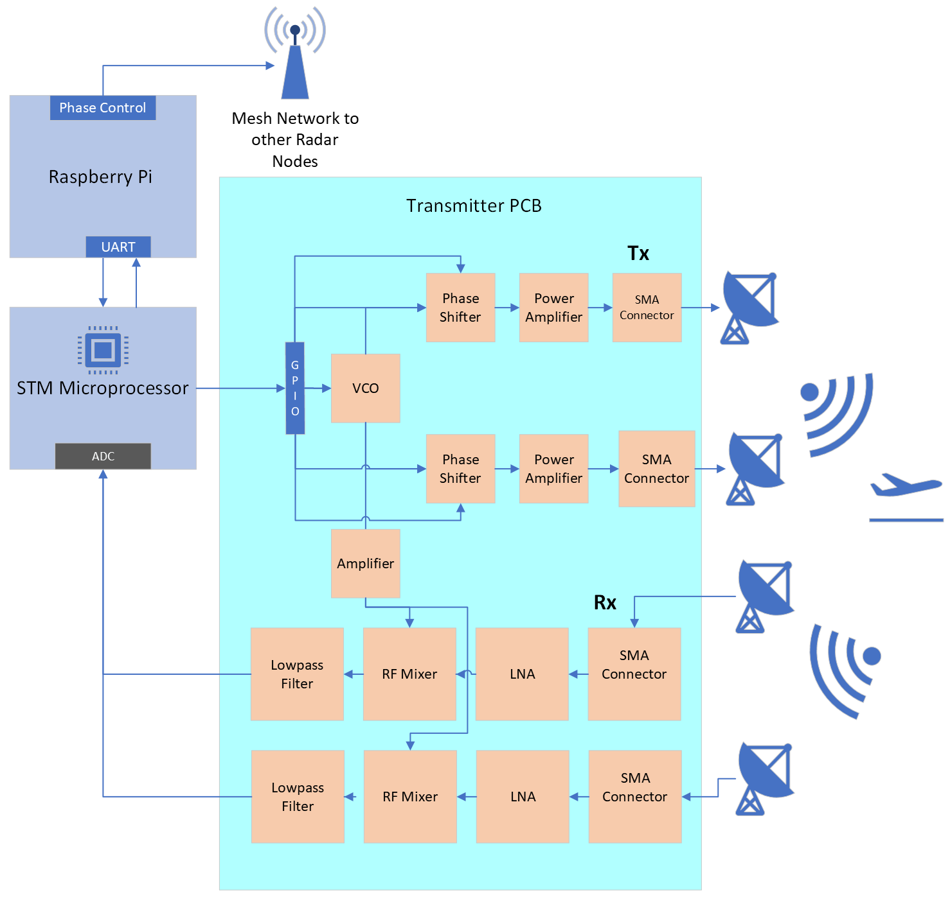
\includegraphics{Diagrams/overview.png}}
\caption{Architecture Overview}
\label{img:projoverview}
\end{figure}

In this chapter, we will go through the architecture of the PCB and show what parts we picked and what purposes they serve.
Figure \ref{img:projoverview} shows the overall architecture of the project.

\section{Voltage Controlled Oscillator (VCO)}
The first step in creating a radar is signal synthesis. You essentially need to create an alternating current signal that can
go through your antenna and radiate out into the air. To reiterate from Chapter \ref{Radar Theory}, higher frequency signals are
important for a better radar resolution, and so it is desired to have a signal that is high in frequency. Naively, at the
beginning of this project we thought we could use a 16 bit DAC to synthesize our signal but after finding out its max clock rate 
was 1 MHz, we realized a DAC was not fit for this. All we needed was something that could create a simple sinusoid at a very
high frequency.

Voltage Controlled Oscillators (VCO) do just this. They take in a "tuning voltage" which corresponds to a certain frequency
of sinusoid which it will output. The circuitry for this is beyond me, but for a good overall guide on VCOs you can check out
DigiKey's article \href{https://www.digikey.com/en/articles/the-basics-of-voltage-controlled-oscillators-vcos}{here}.

Now that we knew how to synthesize our signal, it was important to find a good VCO that had a high output bandwidth. Whatever
bandwidth the VCO has will impact what parts we can get in the other stages of the RF chain since these must be within the VCOs
operating regions. 

\begin{figure}[H]
    \centering
    \scalebox{.7}{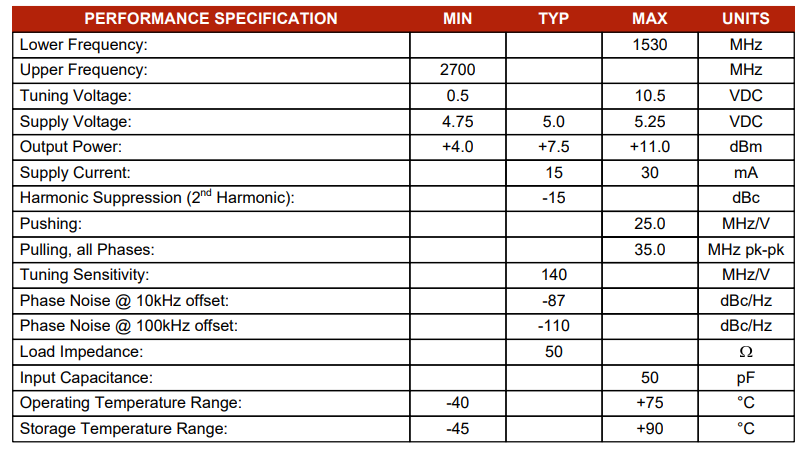
\includegraphics{DatasheetImages/vcotable.png}}
    \caption{VCO Datasheet Table}
    \label{img:vcotable}
\end{figure}
\begin{figure}[H]
    \centering
    \scalebox{.7}{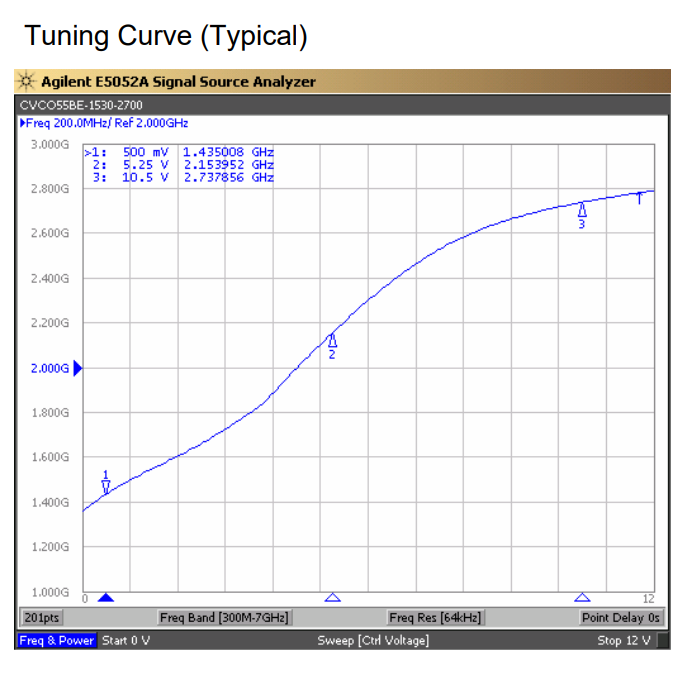
\includegraphics{DatasheetImages/vcotuningtable.png}}
    \caption{Tuning Voltage Graph}
    \label{img:tuninggraph}
\end{figure}

We chose a VCO from Crystek which can be found on Digikey \href{https://www.digikey.com/en/products/detail/crystek-corporation/CVCO55BE-1530-2700/1644030}{here}.
Looking at the specifications table in Figure \ref{img:vcotable}, some good things to look for are first and foremost the frequency
range of the part. It goes from about 1.5-2.7 GHz, which is a pretty wide range and would support a lot of other parts as it also
covers the Wi-Fi band. The second thing to look for is output power. The output power can be a constraint for other parts, since they
might have a absolute limit on their input power, and it is useful to know the output power for finding out how strong your signal will be
once it propogates out of your antenna. Here we can see the output power is around 7.5 dBm, and this will be split four ways. 
Decibels are a logarithmic scale, so we cannot just divide by four but instead use a decibel calculator like \href{https://noisetools.net/decibelcalculator}{this one}.

Now, another key metric is the tuning voltage. Luckily, this Crystek provides a tuning voltage graph found in Figure \ref{img:tuninggraph}
that shows us how the output frequency changes with changes in the tuning voltage. One observation is that it is not linear, meaning
our ramp voltage will not result in a true linear ramp in frequency. Another observation is that our chosen frequency of 1.8 GHz is
around 3.5 volts following the graph. Our STM board that will generate the ramp voltage can by default only go to 3.3 volts, but we
found a workaround to go to 5 volts which allowed us to stick with our decided center frequency.

\section{Power Divider}
As mentioned before, we want to divide the VCO's signal four ways because want it to go to two phase shifters, and two mixers.
At first we thought it was as simple as having one wire split into four, but as we will go over in Chapter \ref{PCB}, impedence
matching is very important in RF circuits. To put it simply, impedance matching ensures that no power is reflected, and this is
important because reflected power means distortions in the signal and power loss. That means we needed a power splitter meant for
splitting an RF signal without causing reflected power. There is not much of note with the part we used which can be found 
\href{https://www.mouser.com/ProductDetail/Mini-Circuits/WP4P1%2B?qs=Imq1NPwxi77kWybHhilv%2Fg%3D%3D}{here}. The main thing is that
it contains the frequency of 1.8 GHz we want to use.

\section{Phase Shifter}
Two of the power dividers split paths will go into phase shifters. The phase shifters are used to make our phased array
of antennas as explained in Chapter \ref{Radar Theory}. They are able to change the phase (add time delay), to the signal 
so that when they propogate through the air they can construct and destruct. The phase shifters we chose can be found
\href{https://www.digikey.com/en/products/detail/psemi/PE44820B-X/5822957}{here}. These are digital phase shifters that have 256
different phases it can apply to the signal. They have a parallel or serial interface we can use to transmit 8 bit words That
will alter the phase of our signal. The interface and its timing diagrams will be explained more in detail in Chapter \ref{Digital Processing}.
All we need to know is that the bandwidth that the chip supports contains 1.8 GHz.

\section{Power Amplifier}
\begin{figure}[H]
  \centering
  \scalebox{.6}{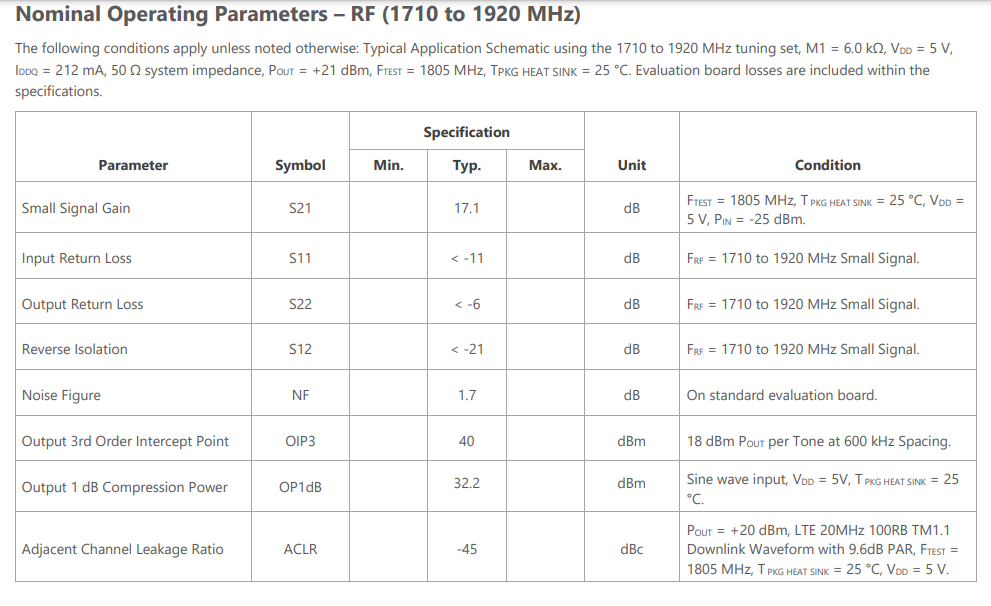
\includegraphics{DatasheetImages/poweramptable.png}}
  \caption{Power Amplifier Table}
  \label{img:poweramptable}
\end{figure}
At this point after the VCO and phase shifter, we want the RF signal to propogate through the air. However, according to the
radar range equation the power of the signal when attenuating through the air attenuates at a power of four which is a lot.
Therefore, we need to make sure our signal is powerful enough to go pretty far. So, we use an RF power amplifier to amplify the
signal. We chose a part from GuerillaRF which can be found \href{https://www.mouser.com/ProductDetail/Guerrilla-RF/GRF5112?qs=ulEaXIWI0c%252Bti188Qa1Now%3D%3D}{here}.
Looking at the table in Figure \ref{img:poweramptable}, we can see some key metrics when looking at power amplifiers. First,
of course we want to make sure it has a bandwidth that supports our chosen frequency of 1.8 GHz. Second, we want to look at the
small-signal gain and Output 1 dB Compression Point or OP1dB. The small-signal gain is the ideal gain that can be reached with a 
low power signal, and is listed as 17.1 dB. The OP1dB is a metric we did not know about and were thankful to find it. With most amplifiers,
gain operates linearly meaning whatever power your input signal is you just add the gain of the amplifier and this will be the resulting power of the signal.
However, at a certain point the amplifier saturates and does not operate linearly anymore, and will essentially cap-off its gain at
the OP1dB limit. For example, with the OP1dB being 32.2 dB, if I input a signal that was 30 dB I would expect a resulting signal of
47.1 dB but this would not be the case. The amplifier ceases to operate linearly after the 32.2 dB mark, and will both distort the signal
and output something weaker than expected. A lot of amplifiers will boast a high gain but have a low OP1dB, so this is definitely something to check for.

\section{Low Noise Amplifier}
\begin{figure}[H]
  \centering
  \scalebox{.7}{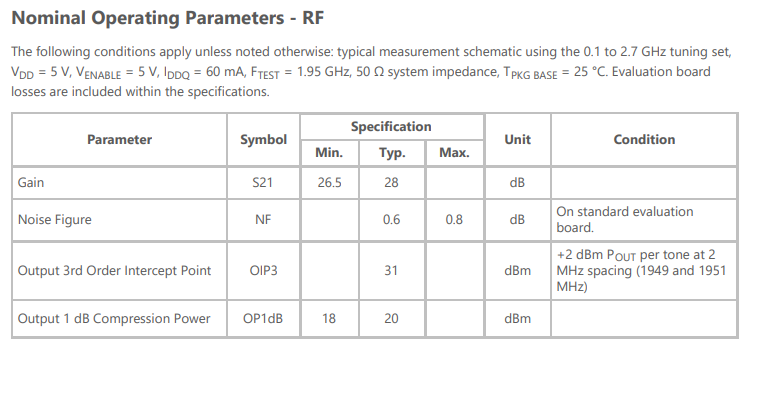
\includegraphics{DatasheetImages/lnatable.png}}
  \caption{Low-Noise Amplifier Table}
  \label{img:lnatable}
\end{figure}

This is the first part that will be placed in the receiver RF chain. According to the Friis equation in Chapter \ref{Radar Theory},
the first stage in the receiver RF chain matters a lot for the noise figure of your system. Therefore, we wanted to find a part
with a low noise figure and high gain, as this will impact our SNR the most. Low noise amplifiers are made for this exact purpose,
where they amplify a small signal with very low noise. The part we chose was \href{https://www.mouser.com/ProductDetail/Guerrilla-RF/GRF2133W?qs=ulEaXIWI0c%2FXgAPwqRmr2A%3D%3D}{this},
which is made by GuerillaRF. By examining the table in Figure \ref{img:lnatable}, we can see that it has a gain of 28 dB,
and a noise figure of .6 dB. We also can look at the OP1dB which has a figure of 20 dB. Since the LNA will be amplifying a signal
straight from an antenna, the signal will be super weak and there is a low likelihood it will reach the OP1dB.

\section{Mixer/LO Amp}
\begin{figure}[H]
  \centering
  \scalebox{.7}{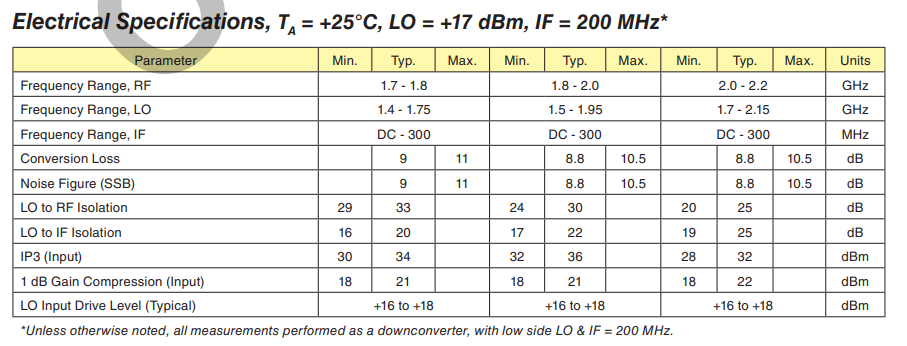
\includegraphics{DatasheetImages/mixertable.png}}
  \caption{Mixer Table}
  \label{img:mixertable}
\end{figure}
\begin{figure}[H]
  \centering
  \scalebox{.7}{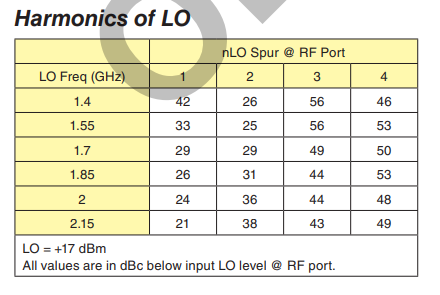
\includegraphics{DatasheetImages/mixerharmonics.png}}
  \caption{Mixer Harmonics Table}
  \label{img:mixerharmonics}
\end{figure}

Now that our received signal is amplified we must down-convert it in order to sample and process it. The process for doing
this is called heterodyning or mixing, and the theory behind this can be found in detail in Chapter \ref{Radar Theory}. 
A mixer has three ports, the local oscillator, RF signal, and output. The local oscillator and RF signal are multiplied
to produce the sum and difference of the LO and RF signals on the output port. We are mainly interested in the difference,
also called the Intermediate Frequency (IF) since it is a low frequency and can be sampled easily.
In our case, we take a copy of the VCO as the local oscillator and then mix this with the amplified return signal 
to produce our intermediate frequency. To achieve this, we used a discontinued mixer from Analog Devices which
can be found \href{https://www.arrow.com/en/products/hmc400ms8etr/analog-devices}{here}. 
Looking at the mixer's specifications table in Figure \ref{img:mixertable}, we can 
see some new properties. The conversion loss is the output IF power delivered minus the available RF input signal power. The
LO to RF Isolation is how much of the local oscillator signal leaks into the RF port, and the LO to IF Isolation is how much
the local oscillator signal leaks into the output port. This is a passive component, meaning it does not require power and
solely operates off the power of the LO and RF signals. Therefore we see in the table that the LO Input must be 16-18 dBm to drive
the mixer. Essentially the local oscillator powers the mixer, and its harmonics will therefore be prominent in the IF port due to
leakage. We can see in Figure \ref{img:mixerharmonics} that at 1.85 GHz the manufacturer tells us the strength of LO harmonics 
up to the fourth order. At the top it says spur which means spurious (unwanted) outputs due to the nonlinearity of the mixer.
Essentially this table tells us that there will be unwanted spectral components in the output, which is something we did not
pay enough attention to and will discuss in Chapter \ref{Issues}.
\begin{figure}[H]
  \centering
  \scalebox{.7}{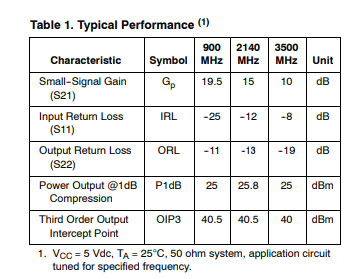
\includegraphics{DatasheetImages/loamptable.png}}
  \caption{LO Amp Table}
  \label{img:loamptable}
\end{figure}

As we said before, the mixer is a passive component which is driven by the LO which needs a power level of 16-18 dBm.
After splitting our VCO's output four ways, we have about a ~2 dBm signal that we must amplify. So, we chose an RF broadband
amplifier from NXP which can be found \href{https://www.digikey.com/en/products/detail/nxp-usa-inc/MMG3014NT1/1971761}{here}. As
we can see in Figure \ref{img:loamptable}, the amp has a gain of around 15 dB for our frequency and an OP1dB of 25.8 dB which is
a lot of headroom.

\section{IF Amplifiers and Filters}
Now, our return signal has been downconverted, but the power of that signal is very weak. As well as this, there are unwanted
spectral components in that signal that are bi-products of the mixer that we need to get rid of. This means we need amplifiers and
filters to make our signal ready to be sampled and processed in the microcontroller. First we used a super simple op-amp
that served as a voltage follower which can be found \href{https://www.digikey.com/en/products/detail/microchip-technology/MCP6001UT-I-OT/562450}{here}.
This was used to create a virtual ground for our biasing. Then we use a dual channel op-amp from TI for our variable gain
amplifier which can be found \href{https://www.mouser.com/ProductDetail/Texas-Instruments/LM2904DR?qs=5BZzbFV4k2vkQqOl3Q8qPg%3D%3D}{here}.

\begin{figure}[H]
  \centering
  \scalebox{.7}{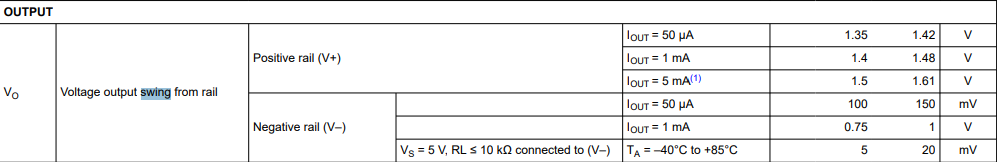
\includegraphics{DatasheetImages/outputswing.png}}
  \caption{Output Swing Characteristics}
  \label{img:outputswing}
\end{figure}

Honestly, when selecting parts we figured all operational amplifiers just acted the same way. However, after printing and manufacturing
we ran into problems which will be discussed in Chapter \ref{Issues} that could have been remedied if we paid more attention to
the Op-Amps we were using. The main problem is that these operational amplifiers are not "Rail-to-Rail".
While rail-to-rail amplifiers guarantee that they do not saturate until the positive and negative voltages you've supplied it,
other amplifiers have what is called voltage swing. As we can see in Figure \ref{img:outputswing}, the range of voltage
that the operational amplifier can achieve is not its rails, but specifies how much lower than its rail it will be. This is 
something to look out for when selecting an Op-Amp.

\begin{figure}[H]
  \centering
  \scalebox{.7}{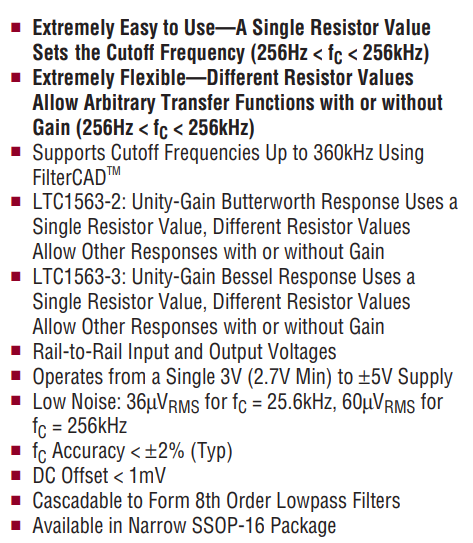
\includegraphics{DatasheetImages/filterspecs.png}}
  \caption{Filter Features}
  \label{img:filterspecs}
\end{figure}

After amplifying the signal, we wanted to filter out unwanted spectral components by using a strong filter. Instead of designing
this ourselves, we decided to use a 4th Order LPF which can be found \href{https://www.digikey.com/en/products/detail/analog-devices-inc/LTC1563-2IGN-PBF/962958}{here}.
By looking at Figure \ref{img:filterspecs}, we can see that this is an integrated circuit with a flexible cutoff frequency.
It also says that it is a rail-to-rail input and output circuit, which is an important feature to note as discussed with the amplifiers.
A fourth order filter just means that this filter has four filters with the same cutoff frequency cascaded upon each other, which
yields a steeper frequency response and attenuates are unwanted signals further.
\chapter{Schematic
\index{Chapter!Schematic}
\index{Schematic}
\label{Schematic}}
\section{ORCad Capture Overview}
ORCad comes with a schematic software called Capture CIS which we used to create our schematics. As a reference to both us and others, this section is
dedicated to providing a small walkthrough to using the software and some nice-to-know features.
\begin{figure}[H]
  \centering
  \scalebox{.3}{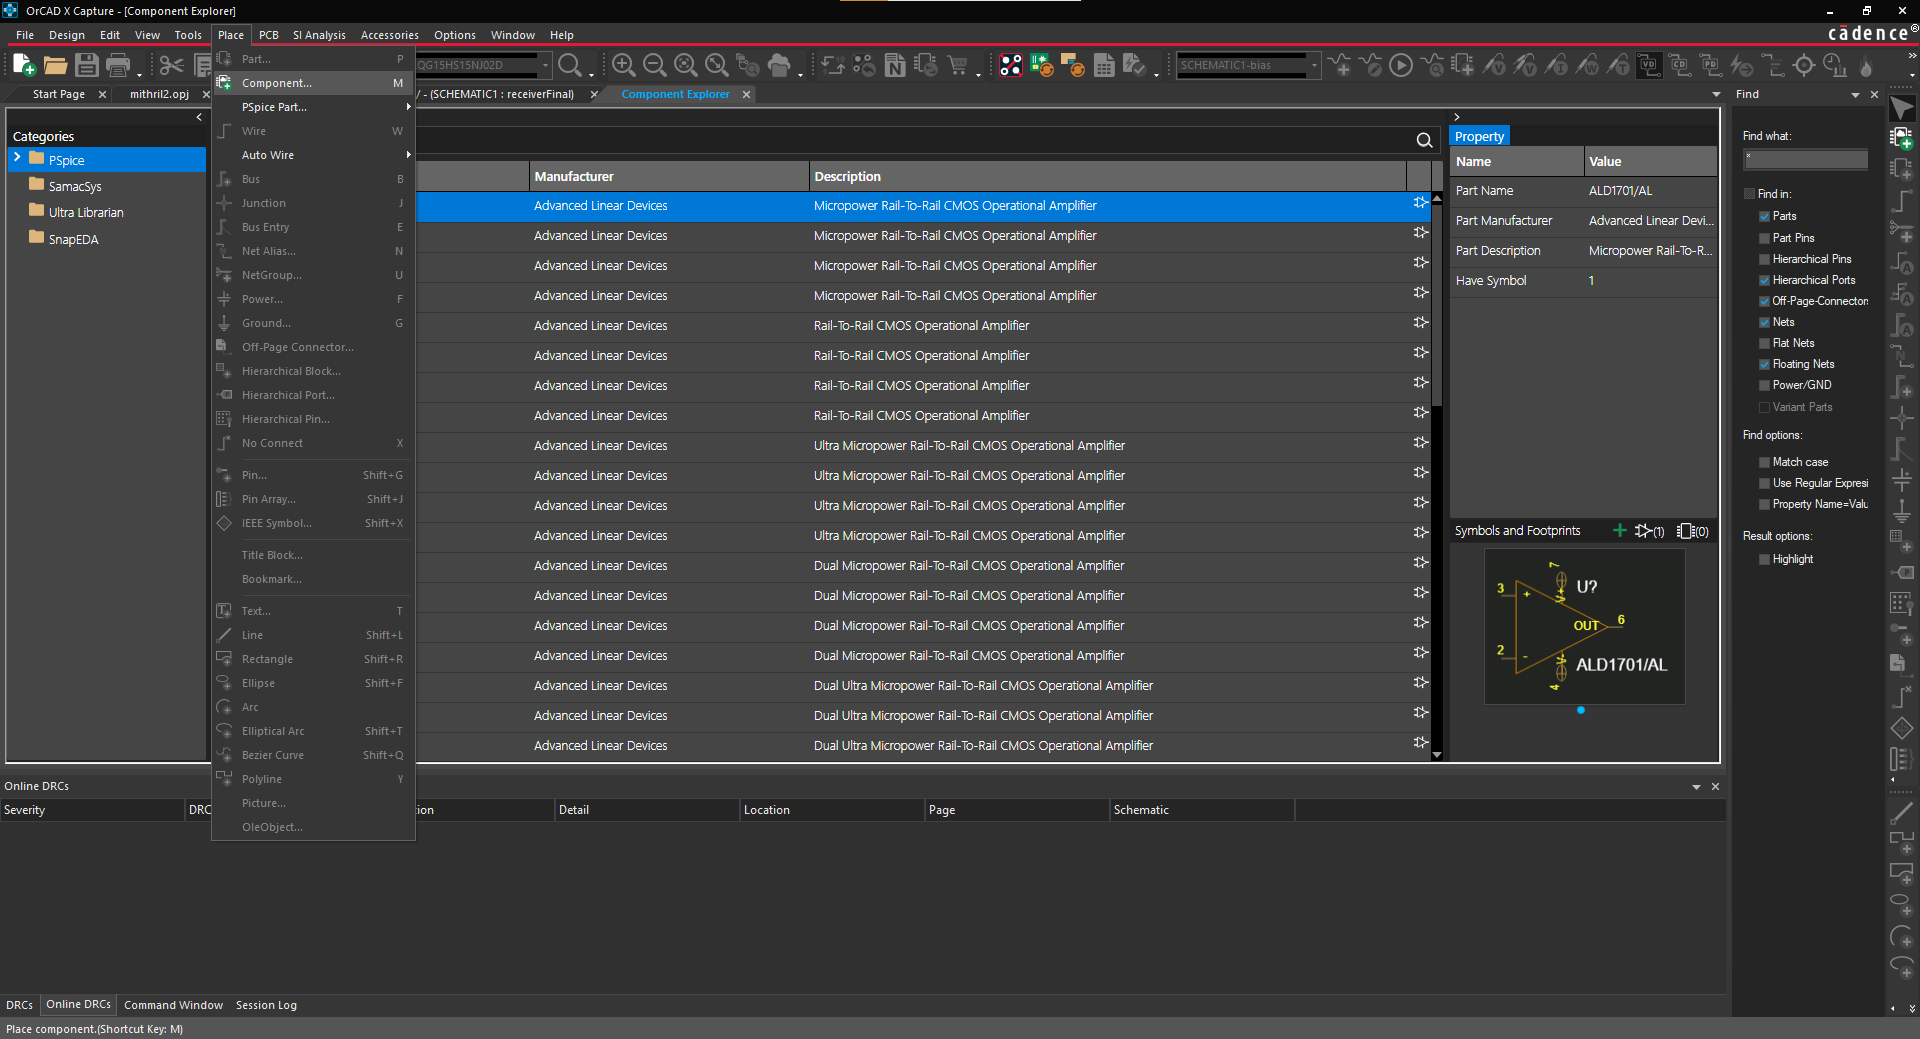
\includegraphics{CaptureImages/ultralib.png}}
\caption{Component Database Search}
\label{img:ultralib}
\end{figure}

The first important feature we found was the component database, which can be seen in Figure \ref{img:ultralib}. By clicking on the icon that has a small chip and cloud will 
take you to this page which contains subdirectories "PSpice" "SamacSys" "UltraLibrarian" and "SnapEDA". PSpice contains parts that
have simulation properties, but we ignored this as we did not know how to use PSpice. The other three are different databases
containing schematic symbols and layout footprints for parts that can be found on major retailers like DigiKey, Mouser, and Arrow.

\begin{figure}[H]
  \centering
  \scalebox{.5}{
\includegraphics{CaptureImages/ultralibexample.png}}
\caption{Schematic/Footprint Examples}
\label{img:ultralibexample}
\end{figure}

You can search for parts in the search fields for the different databases to try to find a part that has a schematic symbol
and footprint available. You can see in Figure \ref{img:ultralibexample} that parts with the symbol and footprint available will
have an amp and chip symbol next to them. The box means there is a 3D CAD model associated with them too. If you cannot find
the symbol and footprint for a part, we recommend going on Mouser and finding the part, then requesting the symbol and footprint.
Usually, the schematic and footprint will be added to SamacSys after a couple of days.

\begin{figure}[H]
  \centering
  \scalebox{.3}{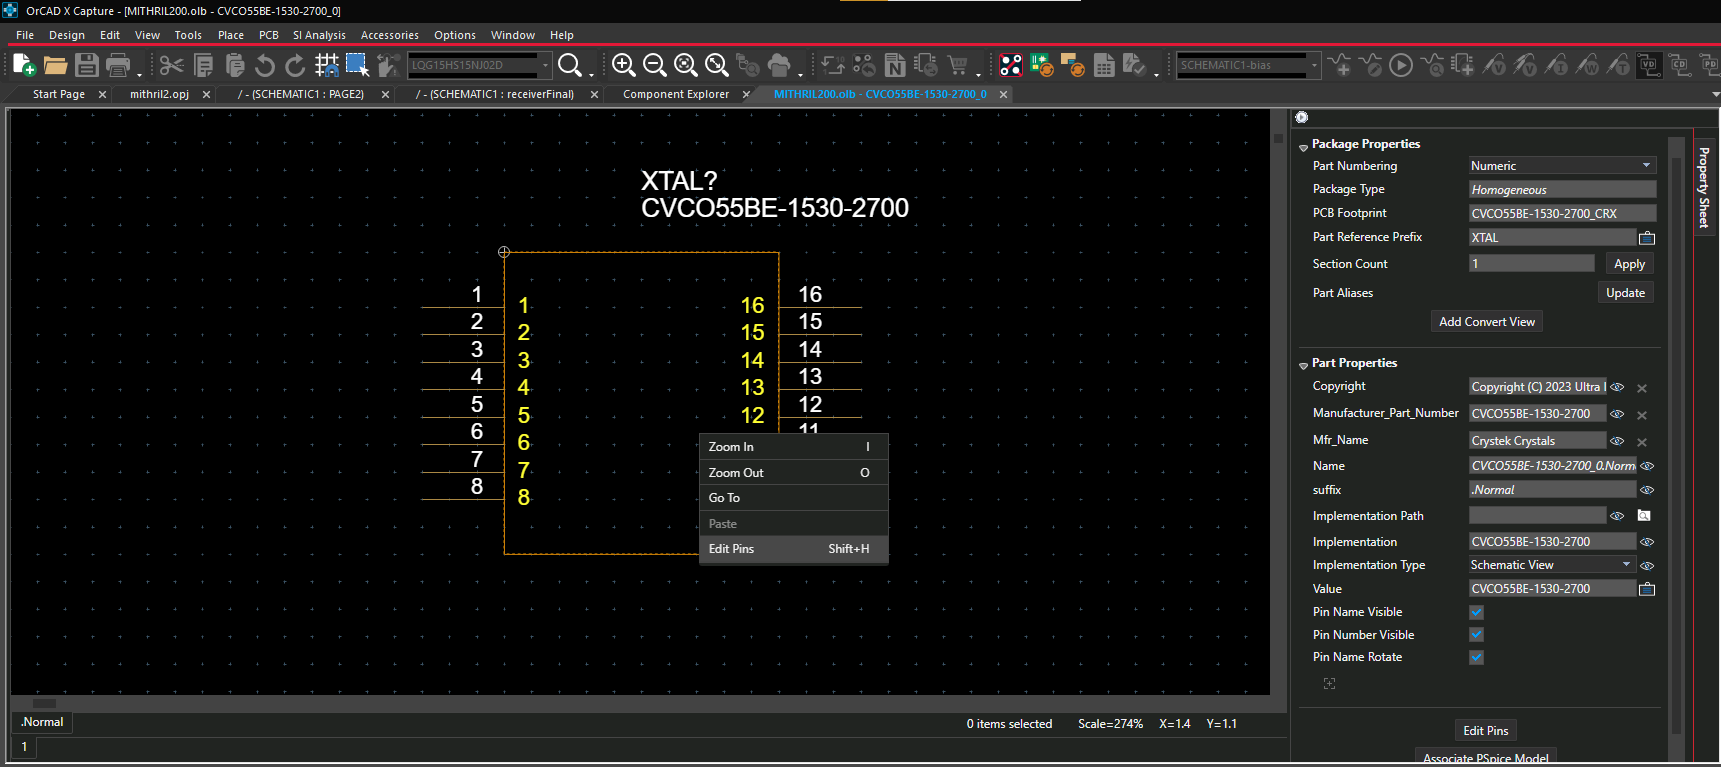
\includegraphics{CaptureImages/editpin.png}}
\caption{Editing Schematic Parts}
\label{img:editpart}
\end{figure}

Sometimes, these symbols and footprints are not correct. If the schematic symbol is incorrectly labeled, you can edit the part,
then click edit pins to make sure all the pins are correctly labeled and numbered as can be seen in Figure \ref{img:editpart}.

\begin{figure}[H]
  \centering
  \scalebox{.3}{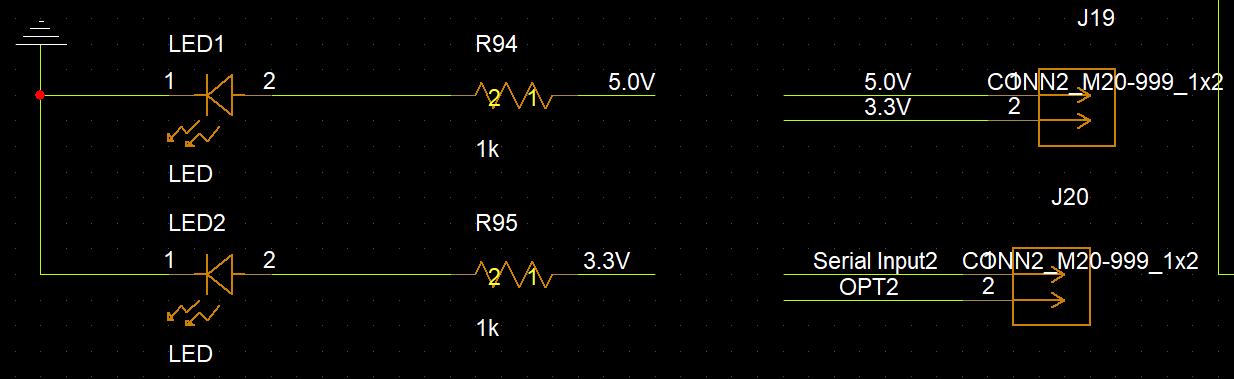
\includegraphics{CaptureImages/wirealias.png}}
\caption{Wires and Net Alias}
\label{img:wirealias}
\end{figure}

Once you've placed your parts down in the schematic, now comes time to connect everything together. To navigate through the
schematic interface, you can use CTRL+Scroll Wheel to zoom in and out, and middle mouse button to scroll left to right.

You can use "w" to enter wiring mode, which lets you place down wires according to your grid size. After wiring, be sure to use
"n" to enter net alias mode and assign aliases to your wires. As can be seen in Figure \ref{img:wirealias}, there are two
non-connected wires both with the alias "5.0V". This effectively connects them since they are under the same alias and will also
label them in the layout when routing. Using the net alias helps with things like power where connecting everything that needs
power with a wire to your power source would make the schematic a mess. In short, all wires with the same net alias are considered
connected.

\begin{figure}[H]
  \centering
  \scalebox{.3}{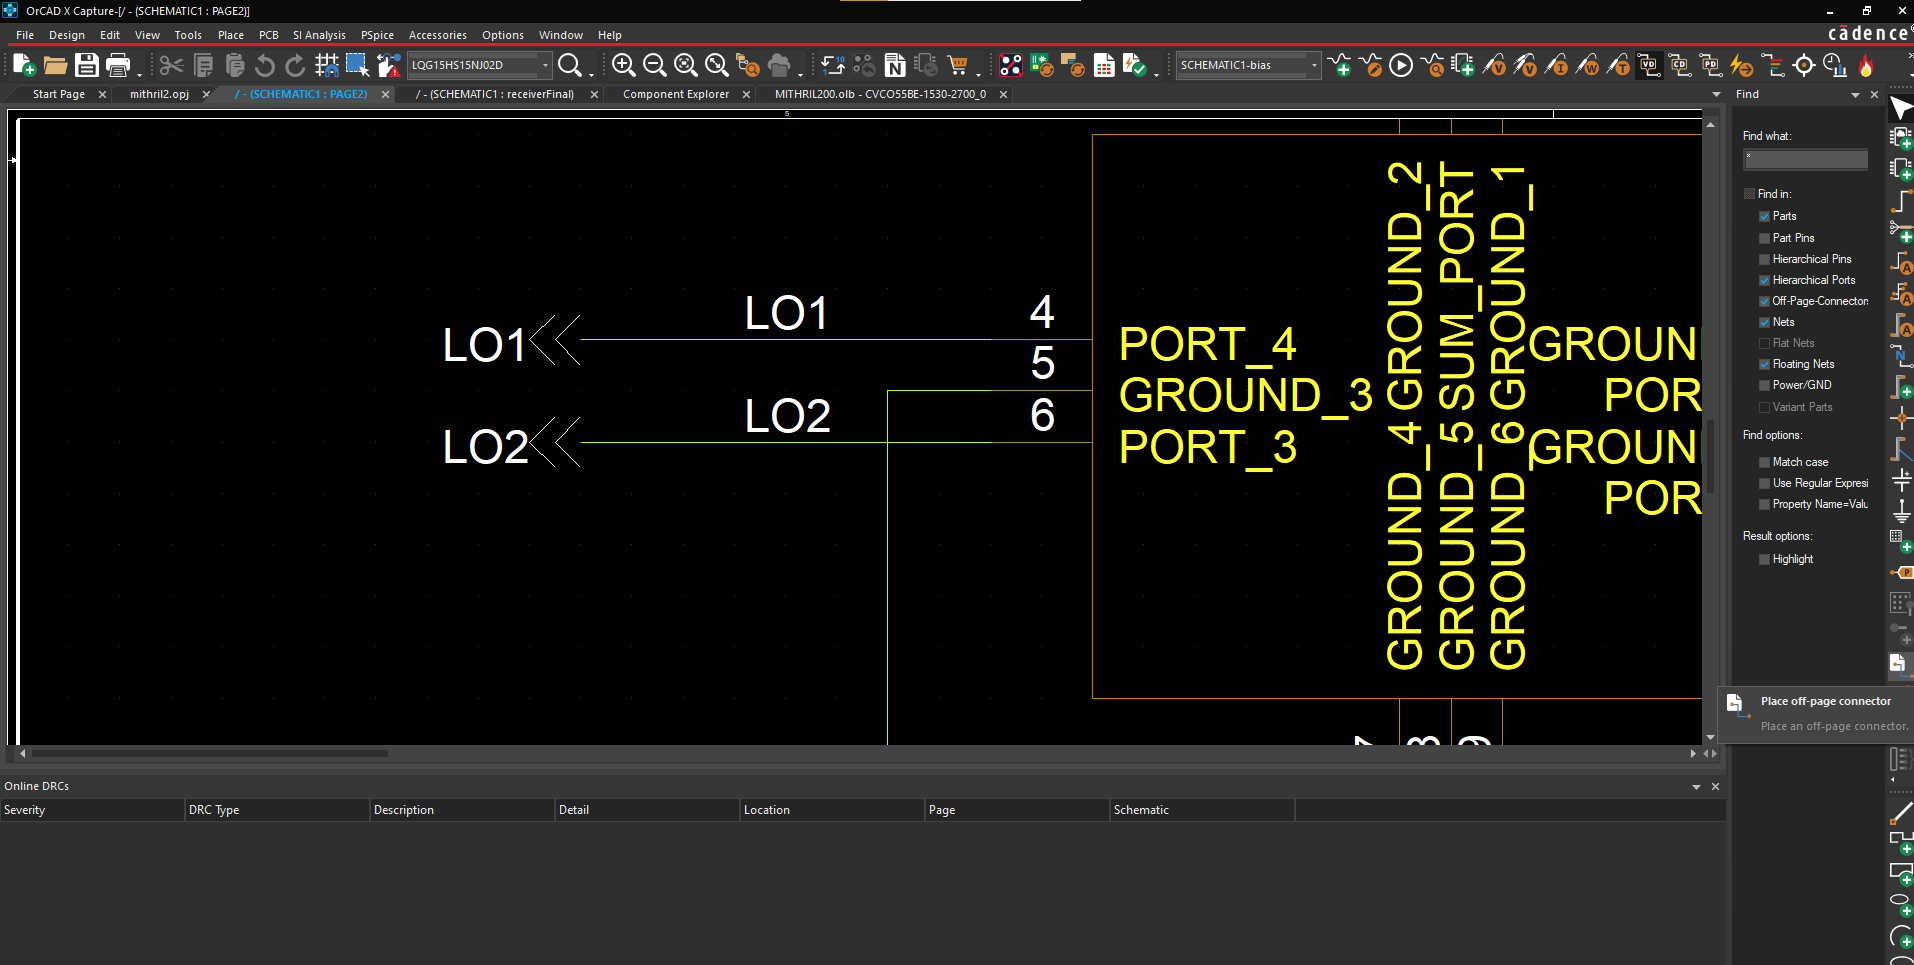
\includegraphics{CaptureImages/offpageconn.png}}
\caption{Off Page Connectors}
\label{img:offpageconn}
\end{figure}

If you run out of room or want to separate your schematics into different pages, you can connect wires from different schematic
pages using off-page connectors as shown in Figure \ref{img:offpageconn}. Connect the off-page connector to a wire and name it
the same on both schematic pages to have the wires connect.

\section{Circuitry Good Practices}
\subsection{DC Blocking and Coupling Caps}
\begin{figure}[H]
  \begin{minipage}{0.5\textwidth}
    \centering
    \scalebox{.3}{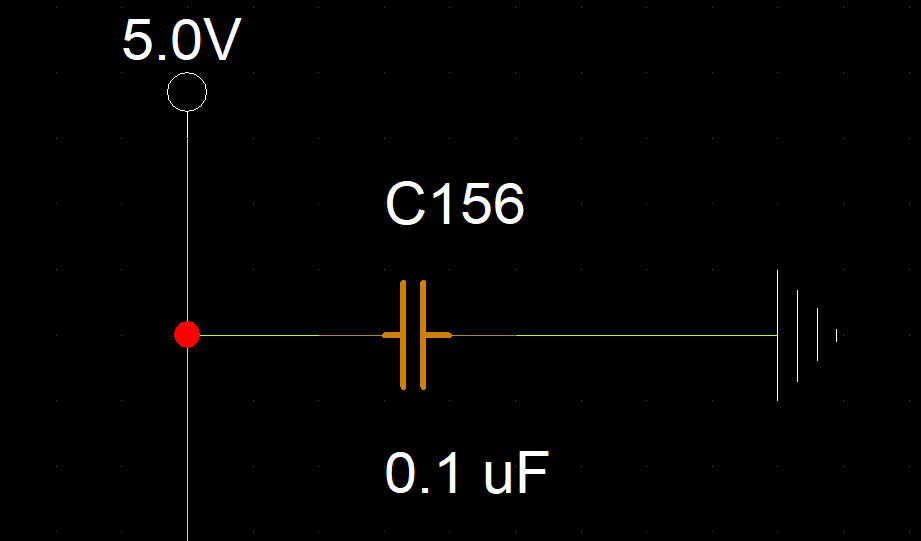
\includegraphics{CaptureImages/coupling.png}}
    \caption{Coupling Capacitor}
    \label{img:couplingcap}
  \end{minipage}
  \begin{minipage}{0.5\textwidth}
    \centering
    \scalebox{.3}{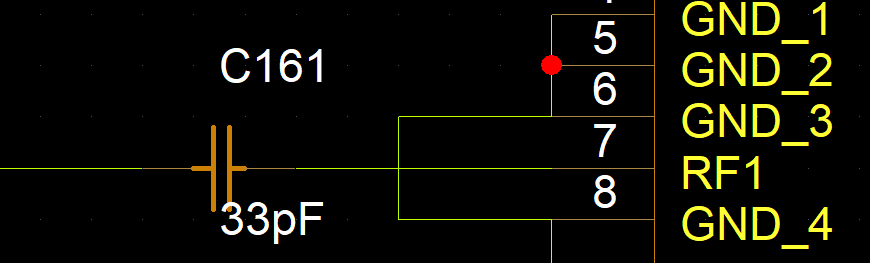
\includegraphics{CaptureImages/dcblocking.png}}
    \caption{DC Blocking Capacitor}
    \label{img:dcblockingcap}
  \end{minipage}
\end{figure}

Two good practices to include in your schematics are coupling and DC blocking capacitors. 

Coupling capacitors are usually used when giving power to some component or chip as can be seen in Figure \ref{img:couplingcap}. It 
can be thought of as a mini low-pass filter, where the capacitance of your coupling capacitor will affect the 
cutoff frequency of the filter. These coupling capacitors should be placed in parallel with the power wire that goes into the chip.

DC Blocking capacitors do the exact opposite, and are usually used when passing a signal from one component to another as can be 
seen in Figure \ref{img:dcblockingcap}. They can be thought of as mini high-pass filters, where the capacitance of the DC Blocking
capacitor affects the cutoff frequency. These are placed in series with the signal wire.
\begin{figure}[H]
\begin{equation}
  C = \frac{1}{2\pi Xf}
  \end{equation}
  \caption{Capacitance of a Coupling or DC Blocking Capacitor}
  \label{eq:capacitance}
\end{figure}
The equation for finding the capacitance of either the coupling or DC blocking capacitor can be seen in Equation \ref{eq:capacitance} 
where C is the capacitance, X is the impedance, and f is the cutoff frequency.
Essentially, a higher cutoff frequency corresponds to a lower capacitance value, and the only difference between the coupling and
DC blocking capacitor is the coupling capacitor passes everything below that cutoff frequency, and the DC blocking capacitor passes
everything above that cutoff frequency.
\subsection{Test Pins and Grounds}
\begin{figure}[H]
  \centering
  \scalebox{.3}{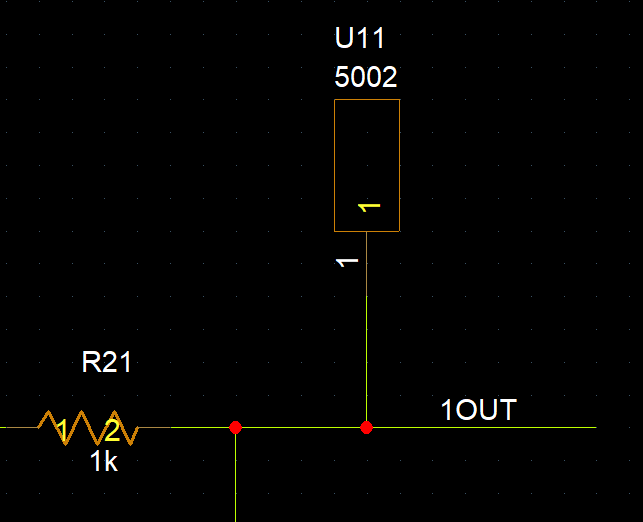
\includegraphics{CaptureImages/testpin.png}}
\caption{Test Pin}
\label{img:testpin}
\end{figure}

Other extremely important things to add are test pins as seen in Figure \ref{img:testpin} and exposures to ground. Credit to
Professor Muresan for telling us to add both of these as they were vital to testing and the operation of the board.

Test pins should be placed in parallel with signal wires so that you can hook in with an oscilloscope and examine what is happening.
Really, after every stage in a signal chain it would be good practice to expose the signal via a test pin or if it is RF with an
SMA connector. This allows you to debug analog things and find out how each stage is affecting your signal. We only added it
in one place and after the fact wished we had placed more test pins so we could see what was happening from component to component.

Ground pins and pads are also really important. We overlooked adding a ground pin which was extremely inconvenient for us, and wished we
had put ample ground pins and pads everywhere on the board. These are necessary if using external components with the board, since
they should have a common ground.

\subsection{Power LEDs}
\begin{figure}[H]
  \centering
  \scalebox{.3}{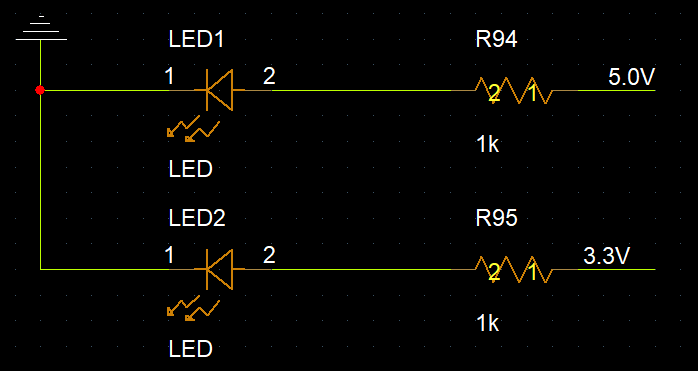
\includegraphics{CaptureImages/leds.png}}
\caption{Power LEDs}
\label{img:led}
\end{figure}

Another nice thing to have are some LEDs connected to power, just so you know at the very least your board is turned on and everything
is receiving power. Having a switch of some sort to block power is also something nice to have which we did not add.

\subsection{Potentiometers}
\begin{figure}[H]
  \centering
  \scalebox{.3}{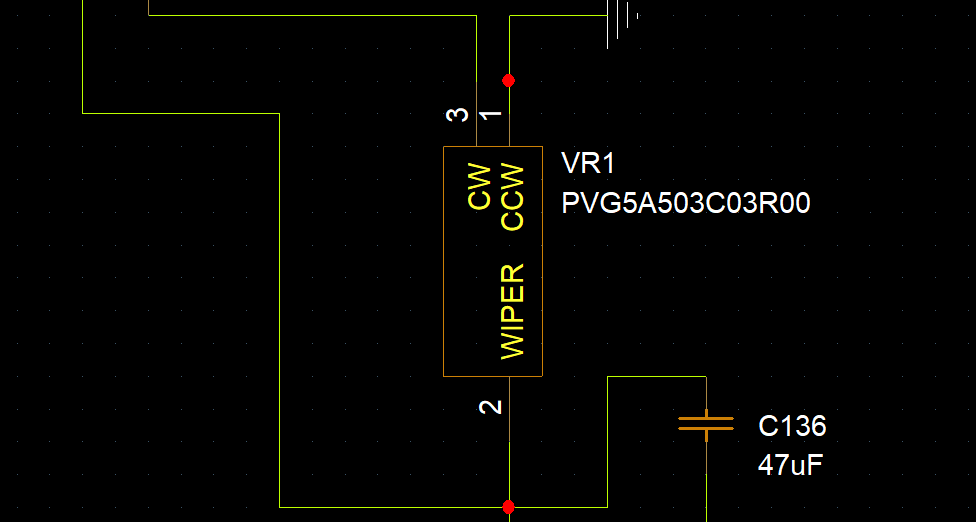
\includegraphics{CaptureImages/pot.png}}
\caption{Potentiometers}
\label{img:pot}
\end{figure}

Another extremely useful thing to add is potentiometers, as can be seen in Figure \ref{img:pot}. In things like amplifying or
filtering stages where resistors can change the cutoff frequency or gain of your circuit, potentiometers are very useful. From
Figure \ref{img:pot}, we can see that potentiometers have three ports: CCW, CW, and Wiper. How potentiometers work is that the
wiper controls the resistance of the potentiometer, and turning it CW will make more signal go in that port, and turning it CCW will
make more signal go into that port (oversimplified explanation). Therefore, it can be set up by just feeding the input to the wiper,
the output to CCW, and CW to ground. This can help with changing gains and cutoff frequencies even after the board is printed and
assembled.

\section{Transmitter}
\begin{figure}[H]
  \centering
  \scalebox{.5}{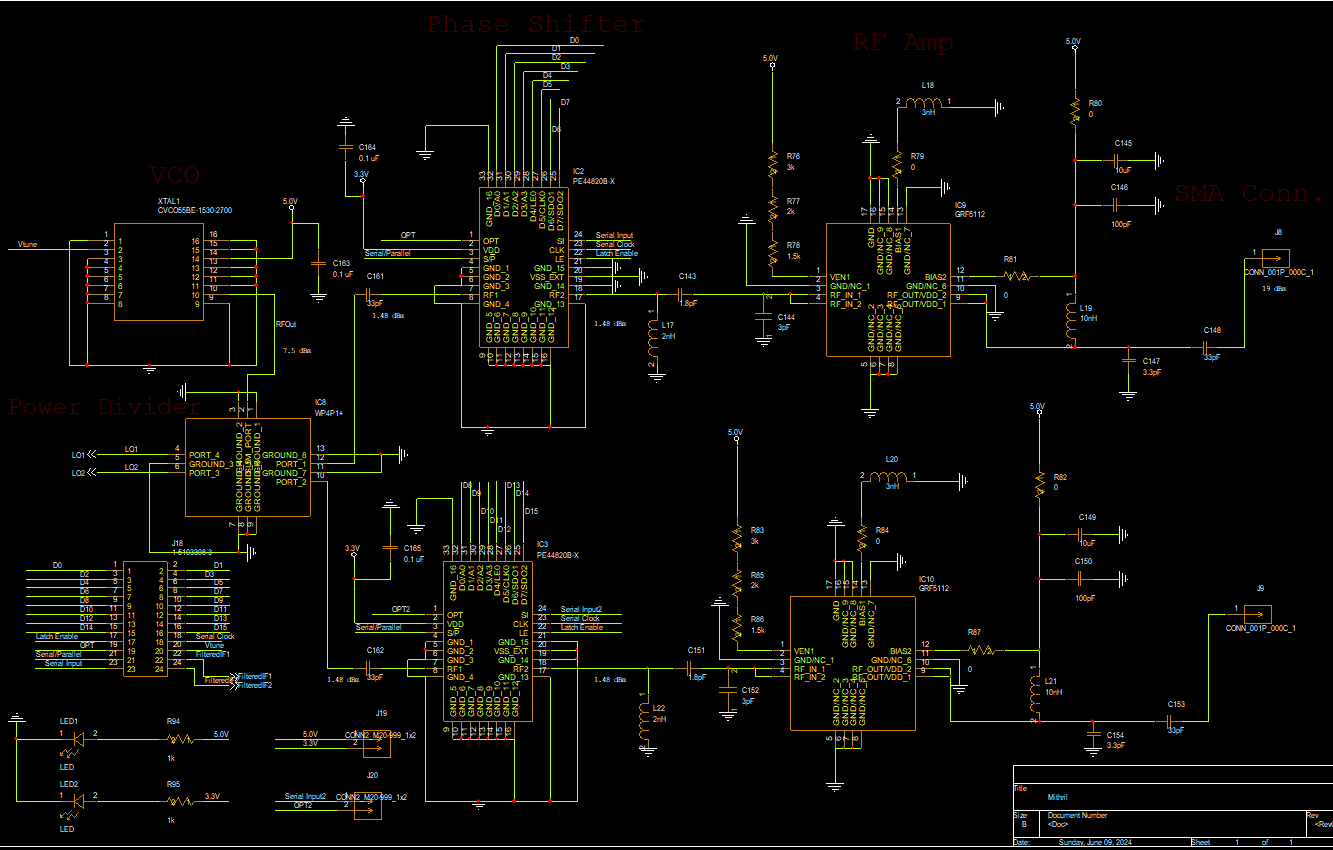
\includegraphics{CaptureImages/transmitterfull.png}}
\caption{Transmitter Schematic}
\label{img:transmitterfull}
\end{figure}
The first step in creating a PCB is fleshing out the schematic. We already decided on what parts to use in Chapter \ref{Part Selection},
and now was the time to create a circuit which interfaces the parts together to make a fully functioning system.
As can be seen in Figure \ref{img:transmitterfull}, the stages of the RF chain are labeled reflecting what was discussed in the
Part Selection chapter. Essentially all of the parts shown here are connected to resistors, capacitors, and inductors according
to the example schematics in their respective datasheets. In the bottom left of the schematic we can see some LEDs
that are connected to power just to make sure the board is being powered and our GPIO connector which will be used to control our
parts. 

The signal path starts with synthesis at the VCO. The VCO connects to 5 volts and is controlled by a tuning voltage will
determine the frequency at the output port of the VCO. This Vtune wire is connected to the GPIO header.

This output signal is then connected to a power divider which splits it four ways. Two of the split signals will
go to the next stage in the RF chain, and the other two are used as local oscillators in the receiver chain. 
This can be seen by two ports of the power divider being connected to off page connectors which can be accessed by the
receiver in another schematic page.

The next stage of the RF chain in the transmitter portion are the phase shifters. The phase shifters will change the phase
of the two identical signals which essentially means a time delay. This causes construction and destruction when the
two signals propogate through the air, and allows for concentrated energy in one direction. We chose 8 bit digital 
phase shifters that have both a serial and parallel interface. The part is connected to 3.3 volts, and has a lot of control and
data pins that we connected to our GPIO header to allow for control by our microcontroller. The phase shifter and its
operation will be discussed more in Chapter \ref{Digital Processing}. 

Finally, the signal passes through our power amplifier with a small signal gain of 17.1 dBm which should help it propogate
through the air for a longer period of time without dissipating. The amplified signal will then propogate through two transmitting
antennas (our small phased array of antennas) to construct and destruct forming a beam of EMF.

\section{Receiver}
\begin{figure}[H]
  \centering
  \scalebox{.5}{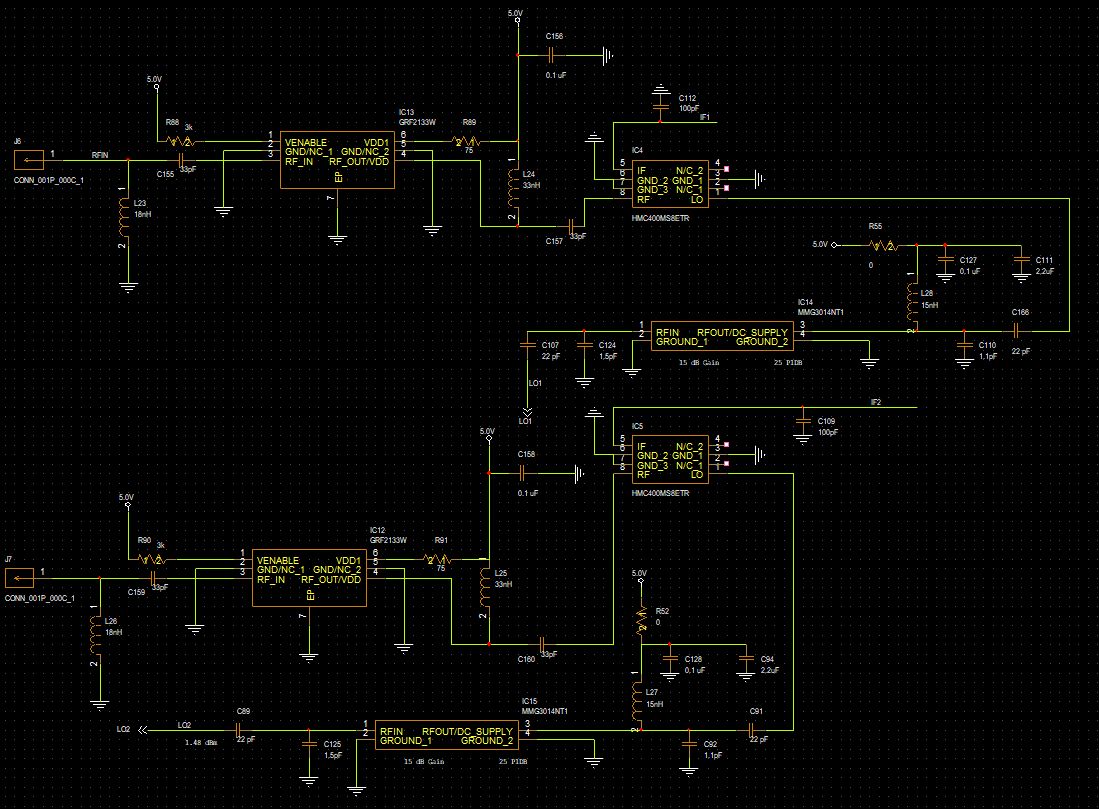
\includegraphics{CaptureImages/receiverfull.png}}
\caption{RF Portion of Receiver Schematic}
\label{img:receiverschem}
\end{figure}
After our signal propogates through the air, it should hit some objects and reflect back to the physical system, and the
goal is to capture this signal and make it digestible to analyze. The first step is capturing the signal, which is accomplished
through the RF portion of the receiving schematic shown in Figure \ref{img:receiverschem}.

First, we have two receiving antennas where the reflected signal should induce a signal in the antennas. We have two
receiving antennas to distinguish the angle of arrival as discussed in \ref{Radar Theory}.

The very small signal induced in the antennas will then pass through a low-noise amplifier which is supposed to amplify our small
signal to be used in the later stages of the chain. The reason a low-noise amplifier is used in a receiving RF chain is because
the first stage of a receiver is the most impactful on its signal-to-noise ratio, or how strong the signal has to be to be
distinguishable from noise. This is discussed more in depth in Chapter \ref{Radar Theory}. This part is powered by 5 volts, and
also has an enable pin that can set the gain of the LNA and disable it if need be. There is also a pin called "EP" which stands
for exposed pad. it is essentially a big ground pad that is used as a heat sink, distributing heat to the ground plane.

After being amplified, the signal is fed into a mixer. The mixer is supposed to output the sum and difference of two RF signals.
One of these is our amplified return signal, the other is a copy of out transmitted signal (LO). This transmitted signal comes from
an off-page connector which is connected to the power divider in the transmitter schematic, and is then amplified by a power
amplifier according to the mixer's LO specifications. The reason it is amplified is because the mixer is a passive
component, meaning it does not use an external power source for its functionality.
The mixer feeds these signals into the RF and LO ports respectively, and
outputs the sum and difference of these signals out of the IF or intermediate frequency port.

\begin{figure}[H]
  \centering
  \scalebox{.5}{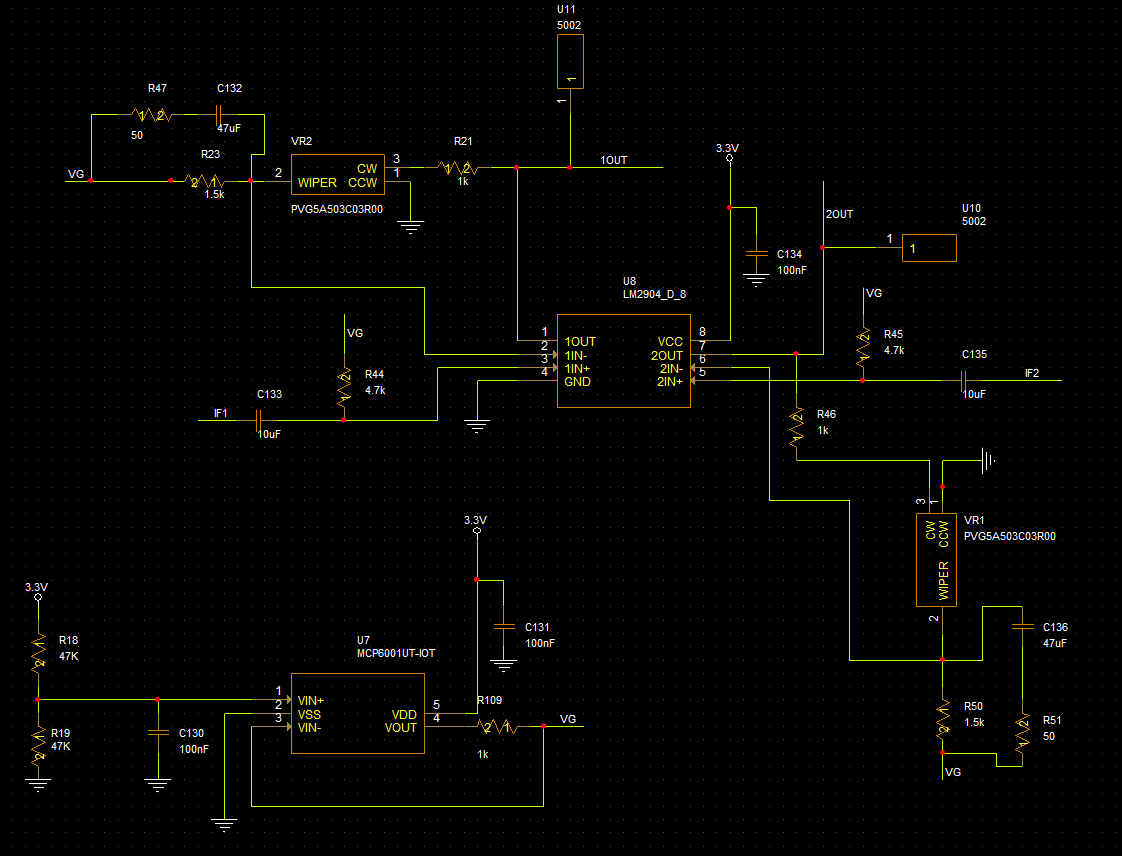
\includegraphics{CaptureImages/basebandamp.png}}
\caption{IF Amplifier Stage}
\label{img:ifamplifier}
\end{figure}

After the sum and difference of our VCO copy (Local Oscillator) and return signal
are outputted from the mixer, we need to do some post-processing to make sense of it.
The first stage of the intermediate frequency processing is in our case
amplification (which turned out to be a bad idea as can be seen in Chapter \ref{Issues}).
As mentioned in \ref{Part Selection}, our mixers output has a reference of 0v or ground.
This means that it contains positive and negative voltage as part of its signal. However,
we decided to use single supply amplifiers. This means its theoretical rails are 0v (ground)
to Vcc (3.3v in this case). Therefore, we need to bias our mixer output around the middle of our rails
to avoid clipping and to take advantage of the full bandwidth of the amp.

The bottom left of Figure \ref{img:ifamplifier} shows our biasing circuit,
which is a simple voltage division using equal resistors and a voltage follower
to keep the voltage steady. This becomes our new "virtual ground", or reference voltage
when dealing with the amplifier. Looking at the dual amp in the center of Figure \ref{img:ifamplifier}, we can see that the mixer output (labeled IF1 and IF2) is
biased with our DC voltage from the biasing circuit, effectively making the new reference 3.3/2 volts. 

\begin{figure}[H]
  \centering
  \scalebox{.5}{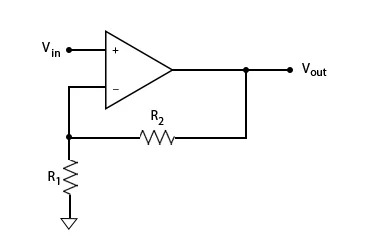
\includegraphics{Diagrams/non-inverting-amp.jpg}}
\caption{Non-Inverting Amplifier Circuit}
\label{img:noninverting}
\end{figure}

The amplifier setup itself was taken from a Finnish engineer named Henrik Forsten whose blog we followed closely and can be found
\href{https://hforsten.com/6-ghz-frequency-modulated-radar.html}{here}. Essentially, it follows a basic non-inverting amplifier
circuit which can be seen in Figure \ref{img:noninverting}. The output of the amplifier feeds to a potentiometer (R2), 
and shares a node with resistance tied to ground (R1) and the negative input of the amplifier. The potentiometer makes this
a variable-gain amplifier, since we can change R2 to different resistance values to fine tune the amplification based on how
small or large the mixer's output is. The ground for the power supply in the amplifier is connected to the power supply, but 
we simply replaced everywhere there would have been ground in the rest of the circuit with our "virtual ground" from the biasing circuit
to make the reference 3.3/2 volts.

\begin{figure}[H]
  \centering
  \scalebox{.5}{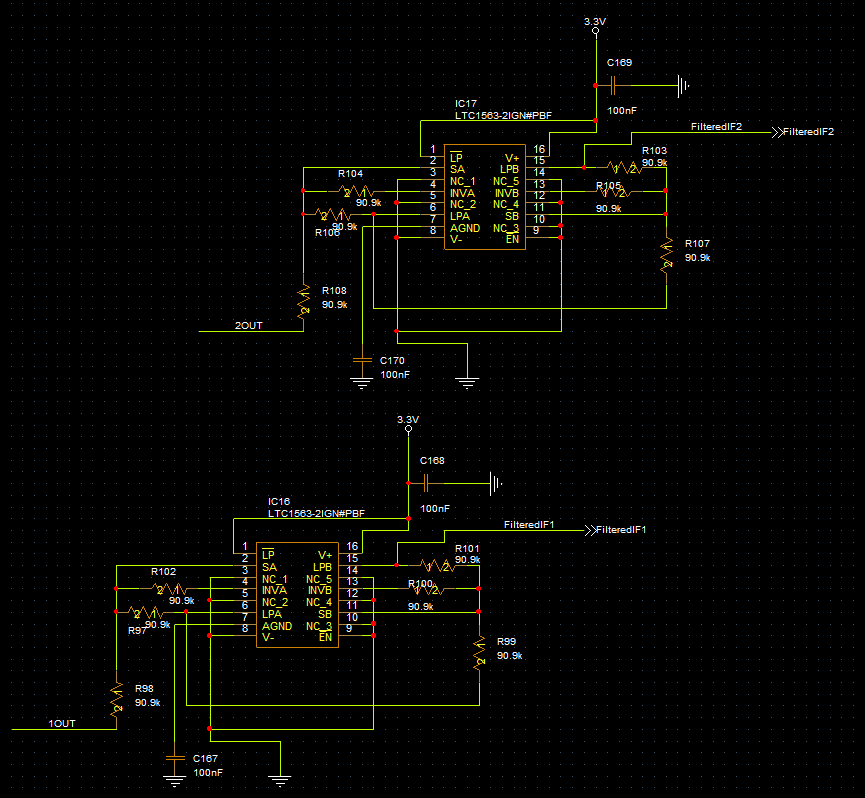
\includegraphics{CaptureImages/filters.png}}
\caption{Low Pass Filters}
\label{img:lpf}
\end{figure}

At this point, our intermediate frequency signal is amplified, but might still have
noise from the antenna or high frequency components from the mixer. In order to remove
these unwanted frequencies from our signal, we want to apply some filtering to only leave
the intermediate frequency of interest. We added fourth-order butterworth LPFs after
the amplifiers to attenuate these other signals. As we can see in \ref{img:lpf}, the 
chip takes multiple resistance values that determine its cutoff frequency.

\begin{figure}[H]
  \begin{equation}
    R = 10k \left(\frac{256kHz}{f_C}\right); \quad f_C = \text{Cutoff Frequency}
    \end{equation}
    \caption{Cutoff Frequency Equation for LPF}
    \label{eq:LPF}
  \end{figure}

The resistances can be determined by Equation \ref{eq:LPF}, and in our case
we used 90.9k resistors to achieve a cutoff frequency of 28 kHz. This filtered
signal then goes to a GPIO pin which will be sampled by a microcontroller.

\chapter{Layout
\index{Chapter!Layout}
\index{Layout}
\label{Layout}}
\section{Intro to PCBs}
Before getting into the meat and potatoes of how to design a PCB, I think it is worthwhile to go over the terms and basics surrounding PCBs.
When starting this project I didn't know anything, and probably still don't, however it helps to know the terms and have context when
watching tutorials and reading documentation, etc.

\subsection{PCB Layers}

\begin{figure}[H]
  \centering
  \scalebox{.7}{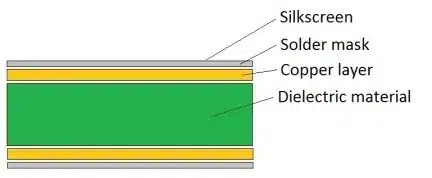
\includegraphics{AllegroImages/layersOverview.jpg}}
\caption{PCB Layers}
\label{img:pcblayers}
\end{figure}

A Printed Circuit Board (PCB) is made up of different materials all stacked up on top each of other, where each of these materials is called
a layer of the PCB. You will also hear the term "stackup" used to describe the amount and kind of layers in one PCB. There are essentially
only four types of layers you need to know, as shown in Figure \ref{img:pcblayers}. The first and most important one is the copper layer.
Copper is a conductor, and so this is the layer in which we place copper where we want to conduct electricity. Whether its for sending power or
signals from one place to another, or placing copper where we want to solder our component pads, this is the place where the actual circuitry is outlined.
You can notice however there are two copper layers in Figure \ref{img:pcblayers}, both of which can have different signals passing through them.
In order to separate the two conductors to prevent shorts, we use a substrate layer, also referred to as a dielectric material. The dielectric
layer goes between copper layers, with one purpose being electrical insulation to keep copper layers from shorting or inducing current in
one another. While it does not conduct electricity, it has a controlled impedance meaning signals won't have weird reactions in different
parts of the board and behavior of signals can be predicted. Different dielectric materials have different dielectric constants, essentially
the number you can use to determine the constant impedance across the board. Now that we have a dielectric and copper layer, we can place a bunch
of copper layers separated by dielectric layers to fit a lot of circuitry in a small space. The third layer we need is the soldermask. The top
and bottom copper layers are exposed to the elements, while all copper layers in the middle are safe within the board. These top and bottom layers
have exposed copper that are subject to things like oxidation, solder shorts between copper areas, and reduces affect of things like moisture.
So, the soldermask is simply a film that goes on top of the top and bottom copper layers to protect it. Finally, the silkscreen layer is just
engraved writing on the soldermask to help humans when assembling the components onto the board. 

\section{Traces and Vias}
\begin{figure}[H]
  \centering
  \scalebox{.7}{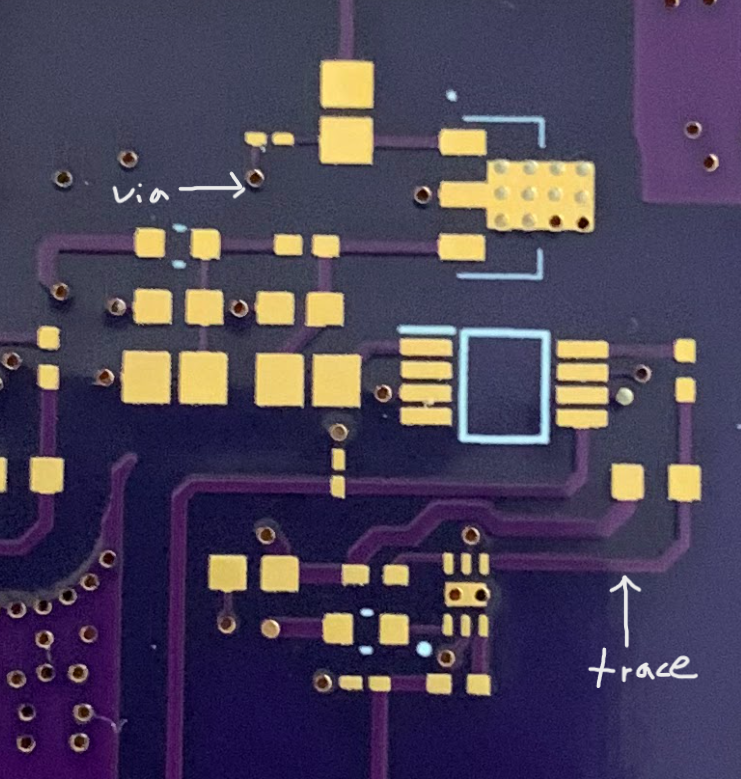
\includegraphics{AllegroImages/tracesandvias.png}}
\caption{Traces and Vias from Mithril Board}
\label{img:tracesandvias}
\end{figure}

In the last section, we mentioned copper layers being where copper is layed down where we want to transmit electricity from one place
to another. This means we have to connect different components, power sources, grounds, etc. with strips of copper which we call traces. As 
can be seen in Figure \ref{img:tracesandvias}, traces can vary in width, orientation, etc., and are basically drawn out by the designer based
on where they want their electricity to go. Their width, orientation, etc. are important, and their affects can be found in Chapter \ref{Radar Theory}.
We also discussed that there can be multiple layers of copper within a board which is great for saving space, but how can we connect one layer
of copper to another when there is an insulated dielectric between them? The answer is vias, which are copper plated holes drilled in the board
that allow for connection of copper in different layers. As can be seen in Figure \ref{img:tracesandvias}, the vias are very small holes which
can vary in diameter and connect to a trace. Like traces, the via diameter can affect its conductive properties in a similar fashion. By using
traces and vias in tandem, we can build out our schematic in a small, consolidated board.

\section{Components}
\begin{figure}[H]
  \centering
  \scalebox{.4}{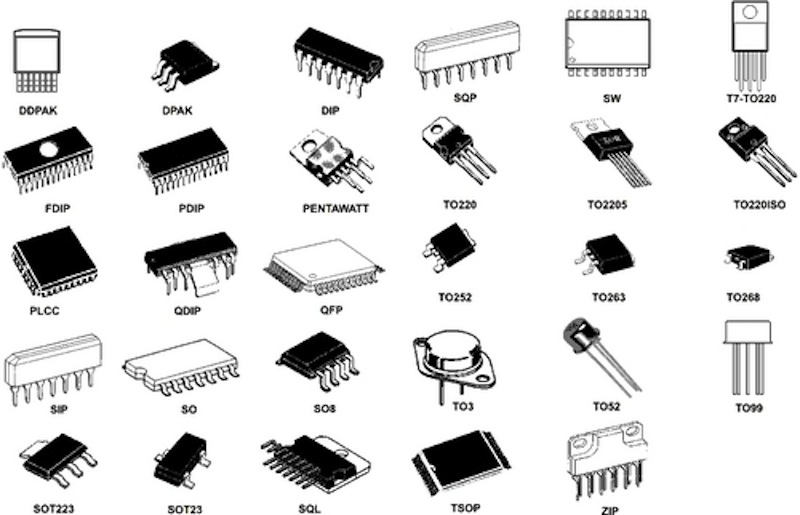
\includegraphics{AllegroImages/componentTypes.jpg}}
\caption{Component Package Types}
\label{img:componentpackage}
\end{figure}
Traces and vias are only useful when they are used with components that execute some task. Whether it be primitive parts like resistors and capacitors
or integrated circuits, components are what make a PCB functional. Components usually come in standardized shapes with standardized pin placements
called packages. Some common package types can be found in Figure \ref{img:componentpackage}. These components will eventually be soldered
onto the PCB, so the designer must put solder pads for the component pins with correct spacing, pitch (width), and orientation. 

\begin{figure}[H]
  \centering
  \scalebox{.4}{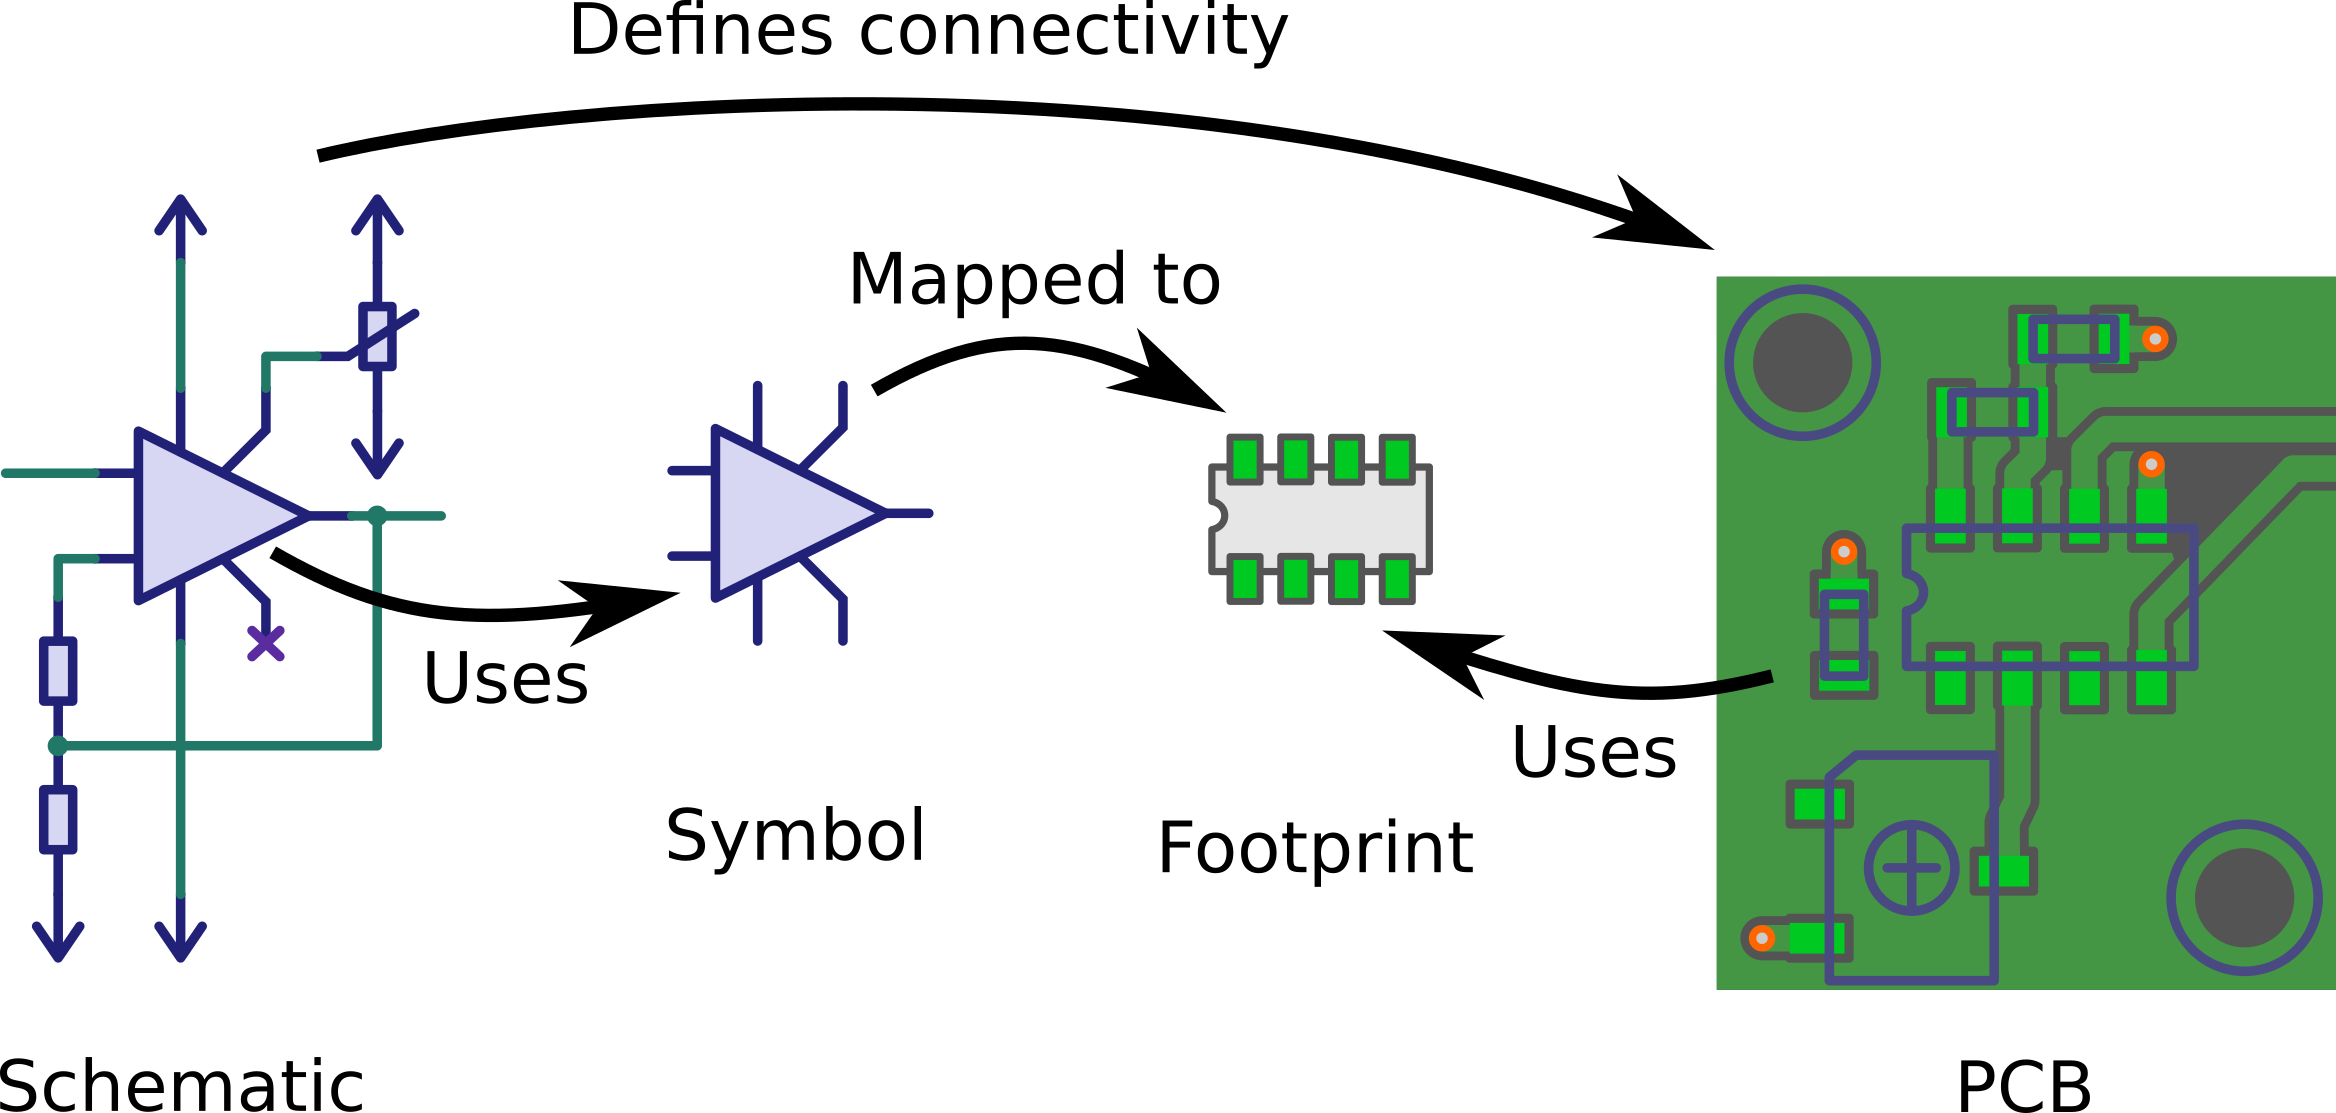
\includegraphics{AllegroImages/footprint.png}}
\caption{Footprint Schematic Symbol Relationship}
\label{img:footprint}
\end{figure}

Instead of the designer drawing all the solder pads with exactly the right dimensions by hand, CAD tools help in creating a "footprint" or a
digital drawing of the size and solder pads of a component. Footprints encapsulate all the physical aspects of a component as mentioned above,
and the designer can map the schematic symbol pins of the same part to the footprint so they know what connects where as can be seen in Figure \ref{img:footprint}.
These footprints follow physical dimensions found in a component's datasheet, and most parts have a footprint out there that someone else made which
you can essentially drag and drop into your design.

\section{Printing and Assembling}
Once you have created your PCB with layers, traces, vias, and components, its time to print the board, order the parts, and assemble the board.
The main deliverables when printing and assembling a board are "Gerbers", a Bill of Materials(BOM), and drill files. Gerbers are ASCII standardized
files that describe all the parts of your PCB (coordinates of parts, orientation of traces, traces on different layers, etc) and are what
printers use to automate the printing process. CAD tools generate these files after your PCB is done, and you can simply send these to your
manufacturer to get your board printed! The BOM describes all the components that are used in your design and makes it easy for you to source
your parts. Drill files specify the locations of vias and chassis treads or any other holes you might have in your board, and again are generated
by your CAD tool.

\section{Allegro Overview}
\begin{figure}[H]
  \centering
  \scalebox{.4}{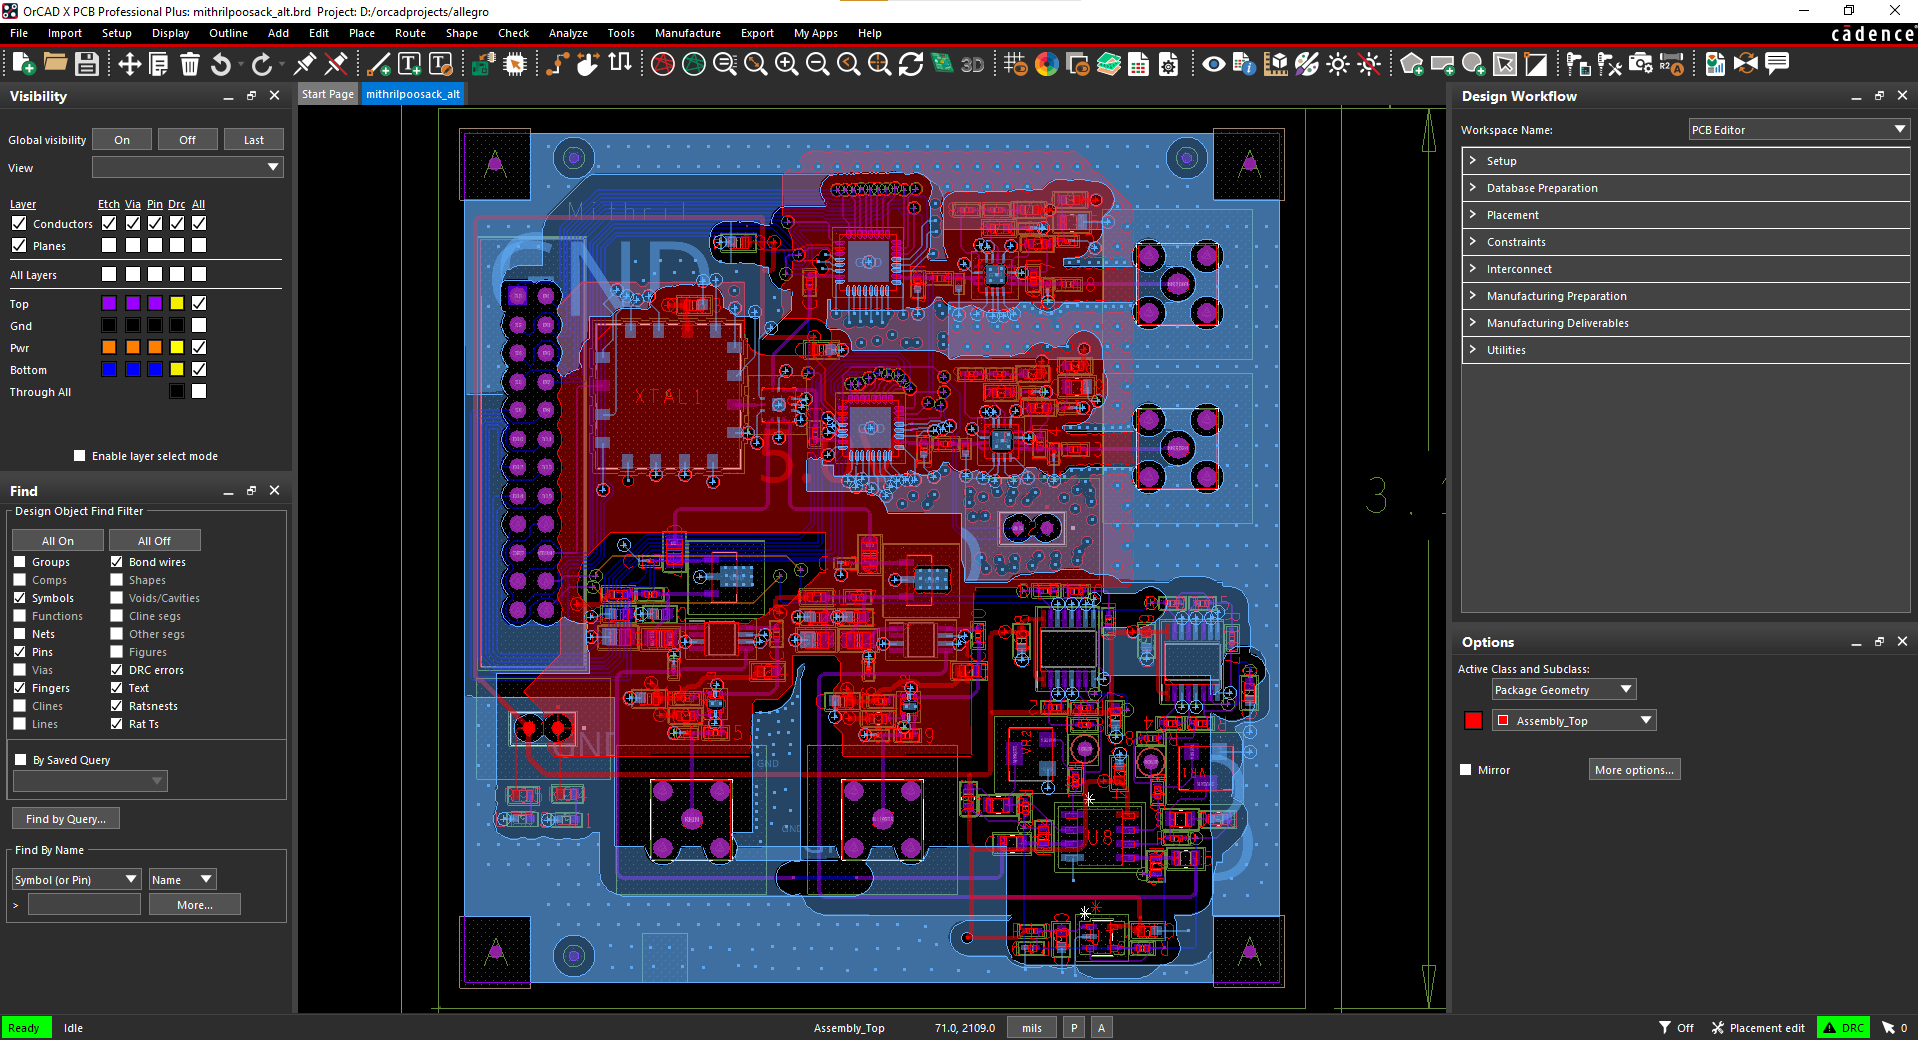
\includegraphics{AllegroImages/layoutfull.png}}
\caption{Allegro Layout}
\label{img:layoutfull}
\end{figure}

First we went over how to create a schematic in Capture CIS, now we will go over Allegro. Allegro is
Cadence's counterpart to Capture which allows you to design a layout for the schematic that can be
printed and assembled to create a functioning printed circuit board.

\begin{figure}[H]
  \centering
  \scalebox{.7}{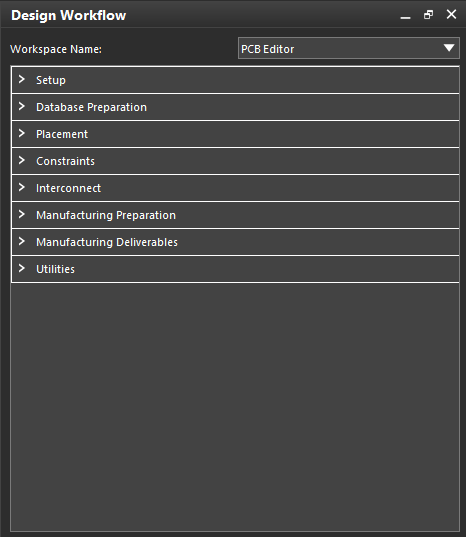
\includegraphics{AllegroImages/designworkflow.png}}
\caption{Design Workflow}
\label{img:designworkflow}
\end{figure}

The most important feature in Allegro is the design workflow. This pane shows all the steps you need to take in order to design a PCB
in Allegro. We will go through all of these panes in the following sections, but make sure to have it open in your Allegro window to quickly
go back and forth from different editing modes.

\begin{figure}[H]
  \centering
  \scalebox{.7}{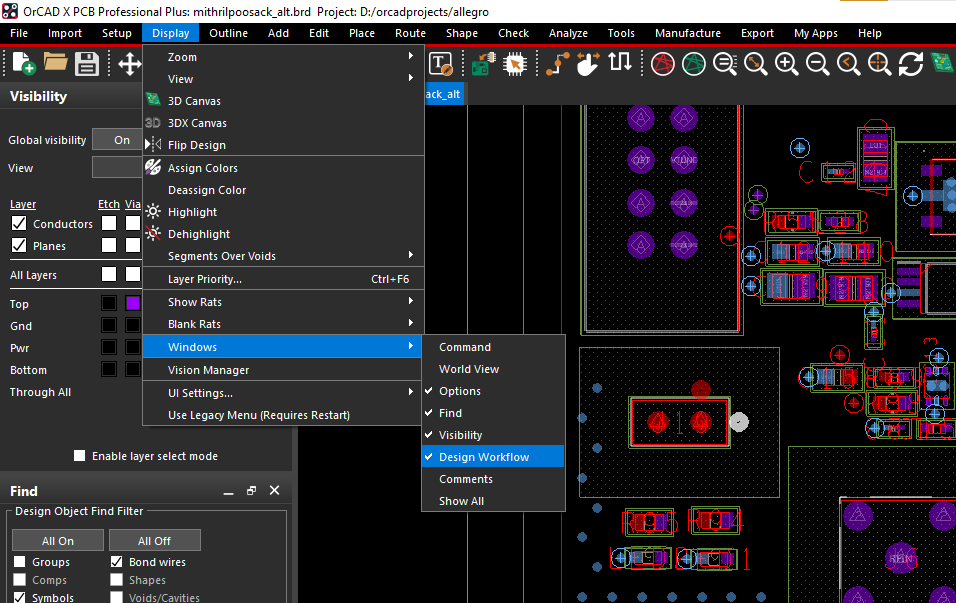
\includegraphics{AllegroImages/windowsTab.png}}
\caption{How to Display Design Workflow}
\label{img:workflowTab}
\end{figure}

If you do not see the design workflow pane in your design, on the top bar navigate to Display, Windows, and then select Design Workflow. You can then drag
and drop the pane to put it wherever you want.

\subsection{Design Setup}

\begin{figure}[H]
  \centering
  \scalebox{.7}{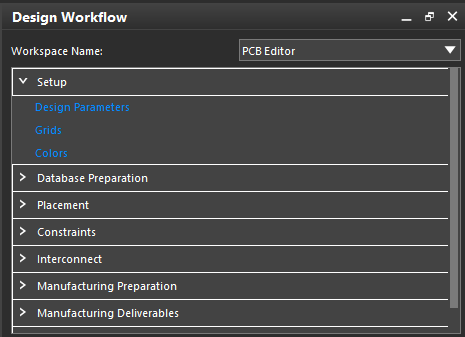
\includegraphics{AllegroImages/setupPane.png}}
\caption{Design Setup}
\label{img:setupPane}
\end{figure}

For Mithril, we followed the design workflow almost verbatim, and this is the workflow we will describe in this tutorial. The first step
is setting up the design to fit our specifications. You can find the setup pane as shown in Figure \ref{img:setupPane}.

\begin{figure}[H]
  \centering
  \scalebox{.7}{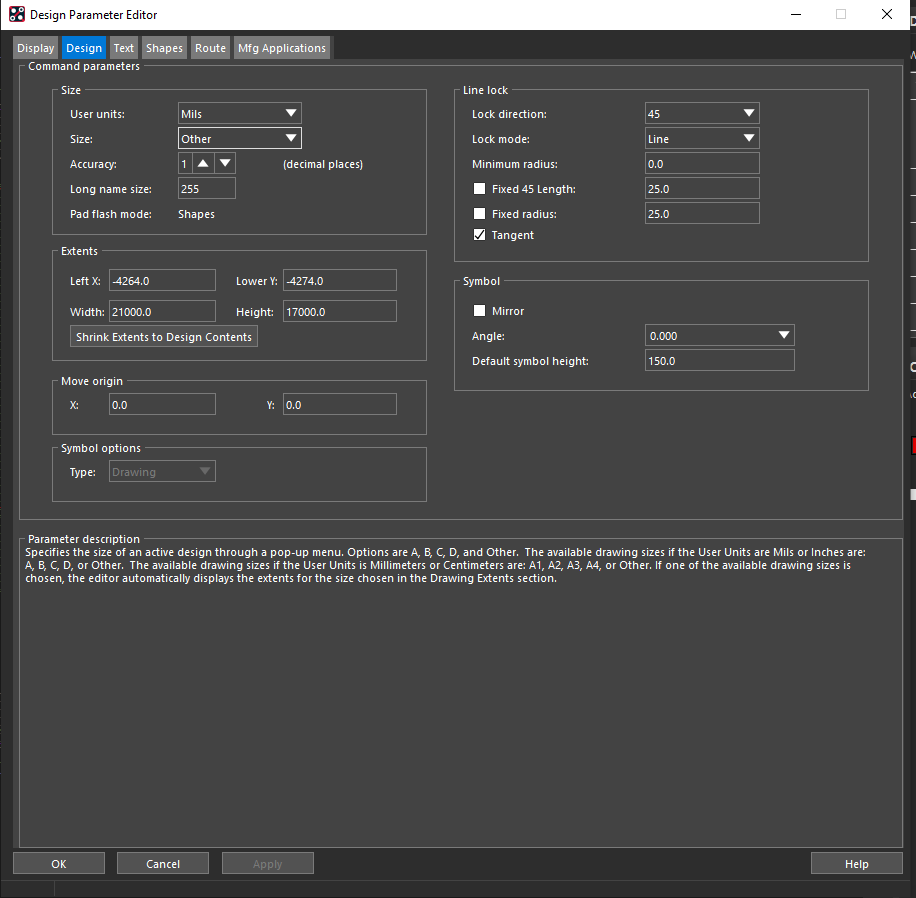
\includegraphics{AllegroImages/designTabSetupPane.png}}
\caption{Design Tab}
\label{img:designTabSetupPane}
\end{figure}

After clicking on "Design Parameters", you can navigate to the Design tab as seen in Figure \ref{img:designTabSetupPane}. Honestly,
this is the only tab that has stuff you want to change. One important thing to change is the user units, which is normally mils (tenth of inch)
or millimeters. You can also switch grids on here, but I prefer them off to be honest.

\begin{figure}[H]
  \centering
  \scalebox{.6}{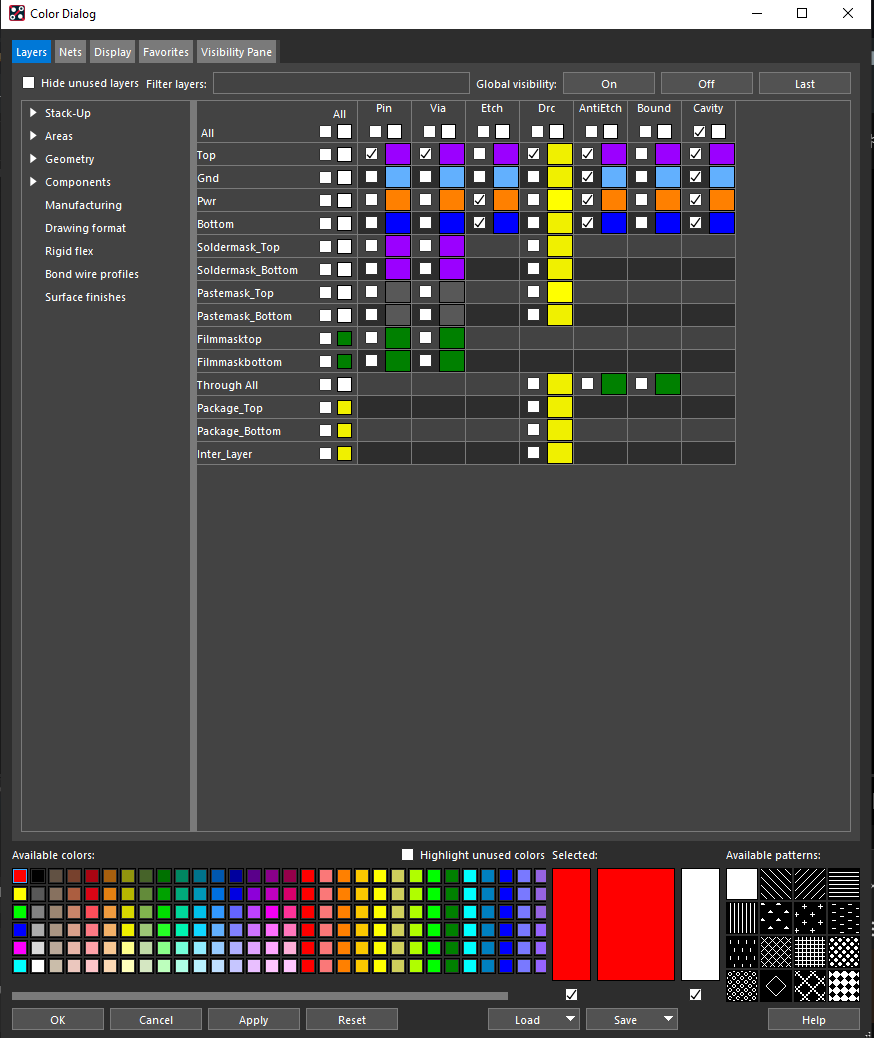
\includegraphics{AllegroImages/colorsTabSetupPane.png}}
\caption{Layer Colors}
\label{img:colorsTabSetupPane}
\end{figure}

The next, and quite frankly a very important tool, is the color tab. This is all really preference, but the defaults in Allegro are pretty bad
and make it hard to see when designing. In the "Layers" tab, there are several drop downs of types of objects that you can set colors for.
You can see my Stack-Up section preferences in Figure \ref{img:colorsTabSetupPane}, and to change colors you click a color on the bottom of the dialog,
then click the little boxes next to a layer and type of object above it. The structure I used was to make everything in a layer the same color except DRC (Design Rule Check)
which points out if you have an error. The first four rows are for my four layers, so I made sure to make them distinct colors. 

\begin{figure}[H]
  \centering
  \scalebox{.6}{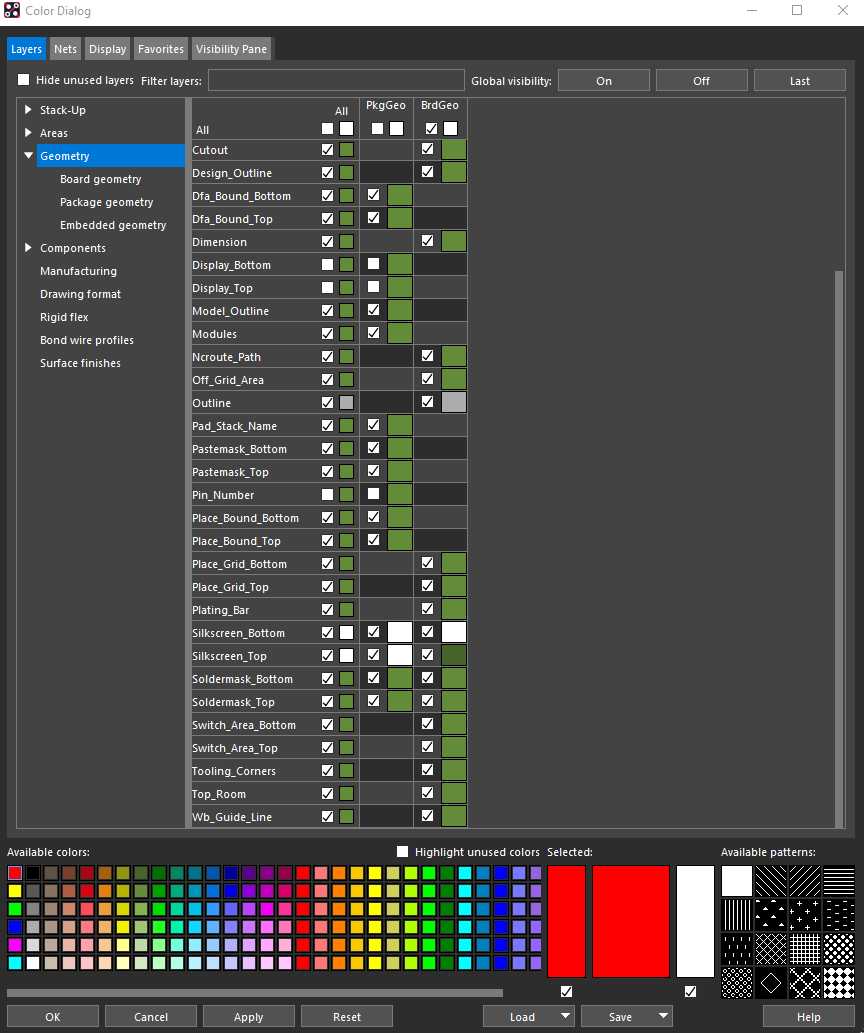
\includegraphics{AllegroImages/colorsGeometry.png}}
\caption{Geometry Colors}
\label{img:geometryColors}
\end{figure}

The layers will make it much easier to distinguish between layers, but there is a lot of bloat text that comes up on the screen with 
Allegro defaults. So, in the "Geometry" tab of the colors dialog I switched off "DisplayBottom", "DisplayTop", and "PinNumber". I also changed
the silkscreen text to white to make it easier to see. This will help with visibility in the long run, and you can see what the geometry
dialog looks like in \ref{img:geometryColors}.

\begin{figure}[H]
  \centering
  \scalebox{.6}{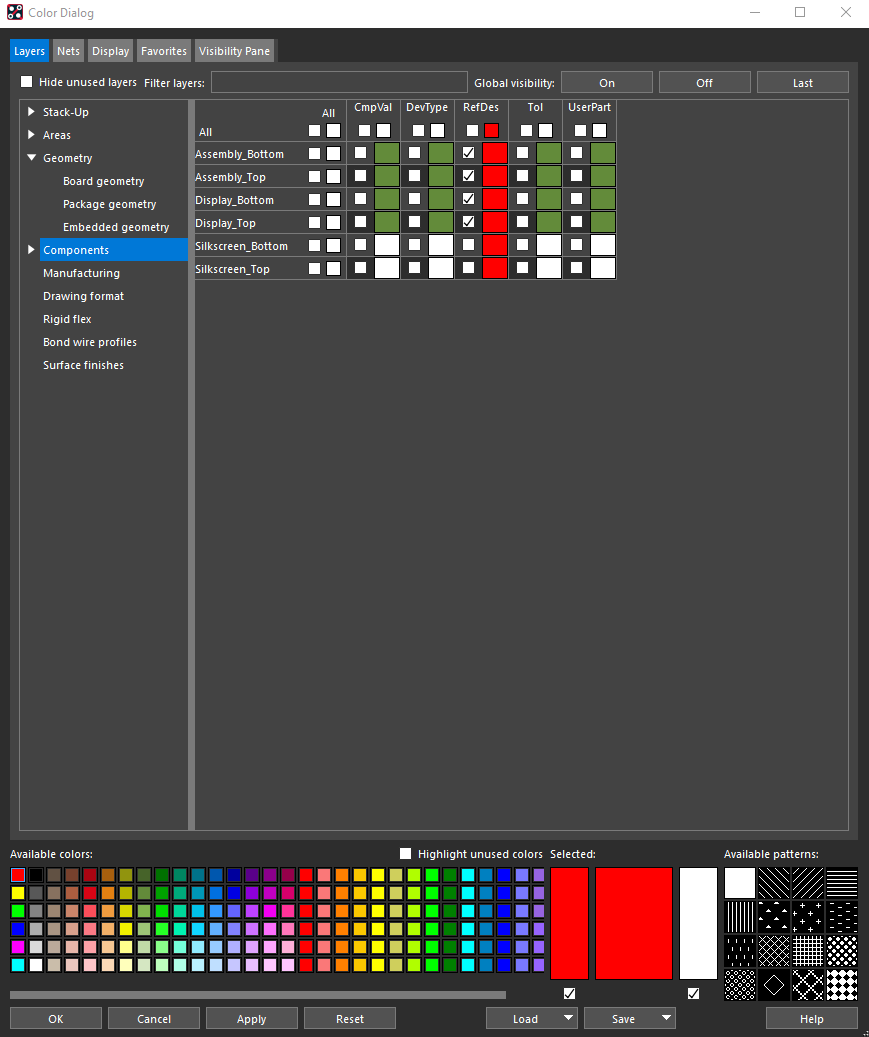
\includegraphics{AllegroImages/colorsComponents.png}}
\caption{Component Colors}
\label{img:componentColors}
\end{figure}

Again, to remove more bloat text navigate to the "Components" tab and uncheck all columns except the "RefDes" column. The RefDes column
will put a text identifier next to every component that is the same as in the schematic, making it easy to identify what is what.

\begin{figure}[H]
  \centering
  \scalebox{.45}{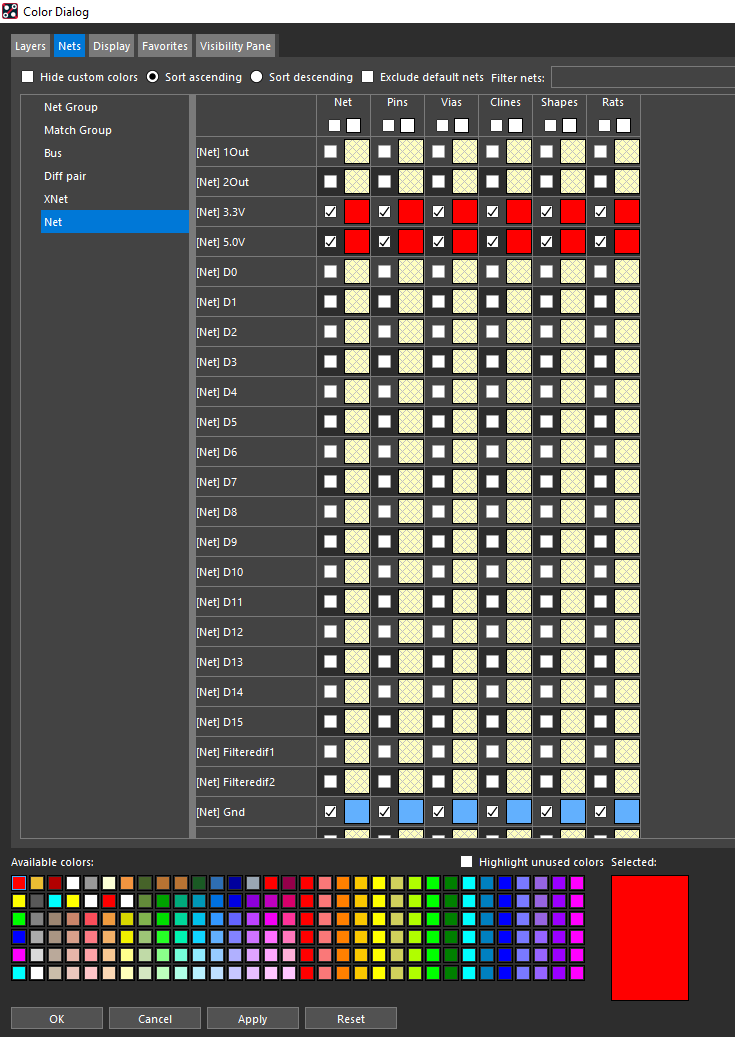
\includegraphics{AllegroImages/netsColors.png}}
\caption{Net Colors}
\label{img:netColors}
\end{figure}

At the top of the colors dialog you can select the nets tab as seen in Figure \ref{img:netColors}. When we draw our traces,
the traces by default will be colored what we selected in the stack-up 

\subsection*{Database Preparation}

\begin{figure}[H]
  \centering
  \scalebox{.45}{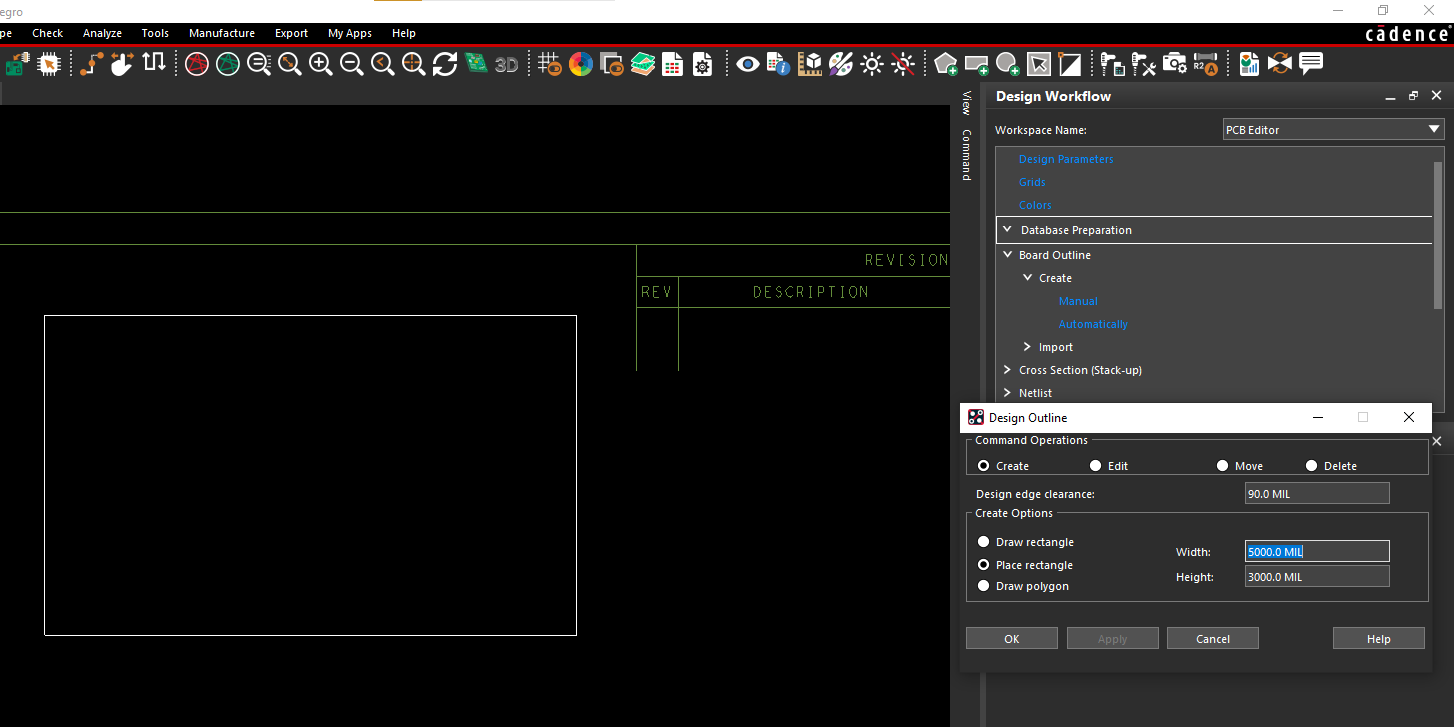
\includegraphics{AllegroImages/boardOutline.png}}
\caption{Board Outline}
\label{img:boardoutline}
\end{figure}

Now that our tool is setup, we can begin in our design. The first section in the Database Preparation is "Board Outline" which can be seen
in Figure \ref{img:boardoutline}. The board outline is for the designer to know the boundary of their future PCB.
Pick the "automatically" option under board outline to get the prompt in the figure. Click create in the prompt,
and then click "Place Rectangle". Now you can enter the design edge clearance, which will dictate how far from the edge of the board you can
place traces or components. Violating the clearance will pop up an error on your design for you to adjust accordingly. After entering your
design clearance, you can enter the length and width of your desired board and a white line will appear that you can move around with your cursor.
Then you can click for the final board and clearance outlines to be drawn.


\chapter{Digital Processing
\index{Chapter!Digital Processing}
\index{Digital Processing}
\label{Digital Processing}}
\chapter{Networking
\index{Chapter!Networking}
\index{Networking}
\label{Networking}}


\chapter{Results
\index{Chapter!Results}
\index{Results}
\label{Results}}
\chapter{Issues
\index{Chapter!Issues}
\index{Issues}
\label{Issues}}

%\bibliography{bibfile}
%\bibliographystyle{unsrt}
%\bibliographystyle{IEEEtran}

%% Initial version by Darian Muresan, Ph.D.
% Edit and adjust as needed.

\documentclass[12pt]{cornell}

% add index support
\makeindex

% graphing programs
\usepackage{color}
\usepackage{psfrag}
\usepackage{verbatim}
\usepackage{fancyhdr}
\usepackage{minted}
%\usepackage{titlesec}
\usepackage{fancyvrb} 
% hyperlink programs
\usepackage[luatex, 
breaklinks=true, 
colorlinks=true,
citecolor=blue,
linkcolor=blue,
menucolor=black,
pagecolor=black,
urlcolor=blue
]{hyperref} % links in pdf
%\usepackage[colorlinks]{hyperref} % links in dvi
\usepackage{listings}
\usepackage{amsfonts} 
\usepackage{amssymb} 
%\usepackage{tabto}

\usepackage{tabularx,colortbl}
\usepackage[chapter]{algorithm} 
\usepackage{algorithmic} 
\usepackage{blindtext}
\usepackage{imakeidx}

% for electronics:
\usepackage[american]{circuitikz}

\definecolor{DarkGreen}{rgb}{0,0.6,0}
\definecolor{mygreen}{rgb}{0,0.6,0}
\definecolor{mygray}{rgb}{0.5,0.5,0.5}
\definecolor{mymauve}{rgb}{0.58,0,0.82}

\usepackage{tocloft}
\usepackage{amsmath}
\usepackage{tcolorbox}
\usepackage{enumitem}
\usepackage{longtable}
%\usepackage{textcomp}
\usepackage{txfonts}

%part for \part titles
%chap for \chapter titles
%sec for \section titles
%subsec for \subsection titles
%subsubsec for \subsubsection titles
%para for \paragraph titles
%subpara for \subparagraph titles
%fig for figure \caption titles
%subfig for subfigure \caption titles
%tab for table \caption titles
%subtab for subtable \caption titles

% update chapter number spacing
\setlength{\cftchapnumwidth}{2em}
\setlength{\cftsecnumwidth}{2.5em}
\setlength{\cftsubsecnumwidth}{3.5em}
\setlength{\cftsubsubsecnumwidth}{4.5em}

\addtolength{\cftsecindent}{0.5em}
\addtolength{\cftsubsecindent}{0.5em}
\addtolength{\cftsubsubsecindent}{0.5em}

%\titlespacing*{\chapter}{0pt}{-50pt}{20pt}
%\titleformat{\chapter}[display]{\normalfont\huge\bfseries}{\chaptertitlename\ 
%\thechapter}{20pt}{\Huge}
%\pagestyle{fancy}
%\pagestyle{cornell}
%
%\rhead{F054-021-0172}
%\chead{Nonlinear Enhancement of Visual Target Detection (AF05-T021)}
%\lhead{GSTI}
%\lfoot{\scriptsize Use or disclosure of data on this page is subject
%to the restriction on the title page of this proposal.}
%\cfoot{}
%\rfoot{\thepage}

\newfont{\Bp}{msbm10}
\newfont{\BpBig}{msbm10 scaled\magstep2}
\newfont{\Sc}{eusm10}
\newfont{\ScBig}{eusm10 scaled\magstep3}
\newfont{\Fr}{eufm10}
\newfont{\FrBig}{eufm10 scaled\magstep1}

% some commands:
\newcommand{\dxi}{{\tt m\_xDeltaInput}}
\newcommand{\dyi}{{\tt m\_yDeltaInput}}
\newcommand{\dci}{{\tt m\_cDeltaInput}}
\newcommand{\dxo}{{\tt m\_xDeltaOutput}}
\newcommand{\dyo}{{\tt m\_yDeltaOutput}}
\newcommand{\dco}{{\tt m\_cDeltaOutput}}
\newcommand{\ttf}[1]{{\tt #1}}
\newcommand{\tbl}[2]{{\begin{tabular}{c} #1 \\ #2 \end{tabular}}}

\newcommand{\urltwo}[2]{\mbox{\href{#1}{\tt #2}}}
\newcommand{\qnorm}[1]{\|#1\|_{\bQ}}
\newcommand{\qdot}[2]{\lrb #1, #2 \rrb_{\bQ}}
\newcommand{\kdot}[2]{\lrb #1, #2 \rrb_{\bf k}}
\newcommand{\tdot}[2]{\lrb #1, #2 \rrb}
\newcommand{\mydiff}[2]{\lrb #1 - #2 \rrb}
\newcommand{\lena}{\textit{lena}}
\newcommand{\barb}{\textit{barbara}}
\newcommand{\boat}{\textit{boat}}
\newcommand{\leaves}{\textit{leaves}}
\newcommand{\rings}{\textit{rings}}
\newcommand{\treg}{\textit{train region}}
\newcommand{\dreg}{\textit{denoise region}}
\newcommand{\oreg}{\textit{overlap region}}
\newcommand{\sil}{\sigma_l^2}
\newcommand{\sn}{\sigma^2}
\newcommand{\bn}{{\mbox{\bf \FrBig N}}}
\newcommand{\n}{\mbox{\Fr N}}
%\newcommand{\bn}{\bf N}
%\newcommand{\n}{N}
\newcommand{\bY}{\textbf{Y}}
\newcommand{\bX}{\textbf{X}}
\newcommand{\bb}{\textbf{b}}
\newcommand{\bu}{\textbf{u}}
\newcommand{\bv}{\textbf{v}}
\newcommand{\by}{\textbf{y}}
\newcommand{\bx}{\textbf{x}}
\newcommand{\be}{\textbf{e}}
\newcommand{\bz}{\textbf{z}}
\newcommand{\bs}{\textbf{s}}
\newcommand{\bw}{\textbf{w}}
\newcommand{\bQ}{\textbf{Q}}
\newcommand{\bphi}{\textbf{$\phi$}}
\newcommand{\lsb}{\left[}
\newcommand{\rsb}{\right]}
\newcommand{\lrb}{\left(}
\newcommand{\rrb}{\right)}
\newcommand{\lcb}{\left\{}
\newcommand{\rcb}{\right\}}
\newcommand{\R}{\mbox{\BpBig R}}
\newcommand{\F}{{\cal F}}
\newcommand{\Fk}{\mbox{\Sc F}}
\newcommand{\bQF}{\textbf{Q}_{\mbox{\Sc F}}}
\newcommand{\N}{{\cal N}}
\newcommand{\xlz}{X_l(z)}
\newcommand{\xhz}{X_h(z)}
\newcommand{\xz}{X(z)}
\newcommand{\pr}{ perfect reconstruction }
\newcommand{\smb}{Smith-Barnwell }
\newcommand{\xw}{X(e^{j\omega})}
\newcommand{\xmw}{X(-e^{j\omega})}
\newcommand{\dw}{D(e^{j\omega})}
\newcommand{\dmw}{D(-e^{j\omega})}
\newcommand{\ew}{E(e^{j\omega})}
\newcommand{\emw}{E(-e^{j\omega})}
\newcommand{\fw}{F_0(e^{j\omega})}
\newcommand{\fmw}{F_0(-e^{j\omega})}
\newcommand{\hoz}{H_1(z)}
\newcommand{\hzz}{H_0(z)}
\newcommand{\goz}{G_1(z)}
\newcommand{\gzz}{G_0(z)}
\newcommand{\hzw}{H_{0}(e^{j\omega})}
\newcommand{\hzmw}{H_{0}(-e^{j\omega})}
\newcommand{\hzcw}{H_{0}(e^{-j\omega})}
\newcommand{\how}{H_1(e^{j\omega})}
\newcommand{\homw}{H_1(-e^{j\omega})}
\newcommand{\gzw}{G_0(e^{j\omega})}
\newcommand{\gzmw}{G_0(-e^{j\omega})}
\newcommand{\gow}{G_1(e^{j\omega})}
\newcommand{\gomw}{G_1(-e^{j\omega})}
\newcommand{\wl}{e^{-jwL}}
\newcommand{\aqua}{\textit{AQua with OR }}
\newtheorem{theorem}{Theorem}
\newtheorem{lemma}{Lemma}
\newtheorem{corollary}{Corollary}
\newtheorem{claim}{Claim}
\newtheorem{definition}{Definition}
\newenvironment{proof}{\noindent{\em Proof.}}{\ \hfill Q.E.D.}
%\newtheorem{moduleCount}{L}
\newcommand*{\labelfile}[1]{%
  \label{file:#1}%
}

\lstset{ %
  backgroundcolor=\color{white},   % choose the background color; you must add \usepackage{color} or \usepackage{xcolor}
  basicstyle=\footnotesize,        % the size of the fonts that are used for the code
  breakatwhitespace=false,         % sets if automatic breaks should only happen at whitespace
  breaklines=true,                 % sets automatic line breaking
  captionpos=b,                    % sets the caption-position to bottom
  commentstyle=\color{DarkGreen},    % comment style
  deletekeywords={...},            % if you want to delete keywords from the given language
  escapeinside={\%*}{*)},          % if you want to add LaTeX within your code
  extendedchars=true,              % lets you use non-ASCII characters; for 8-bits encodings only, does not work with UTF-8
  %frame=single,                   % adds a frame around the code
  keepspaces=true,                 % keeps spaces in text, useful for keeping indentation of code (possibly needs columns=flexible)
  keywordstyle=\color{blue},       % keyword style
  language=C++,                    % the language of the code
  morekeywords={*,...},            % if you want to add more keywords to the set
  numbers=left,                    % where to put the line-numbers; possible values are (none, left, right)
  numbersep=5pt,                   % how far the line-numbers are from the code
  numberstyle=\tiny\color{mygray}, % the style that is used for the line-numbers
  rulecolor=\color{black},         % if not set, the frame-color may be changed on line-breaks within not-black text (e.g. comments (green here))
  showspaces=false,                % show spaces everywhere adding particular underscores; it overrides 'showstringspaces'
  showstringspaces=false,          % underline spaces within strings only
  showtabs=false,                  % show tabs within strings adding particular underscores
  stepnumber=1,                    % the step between two line-numbers. If it's 1, each line will be numbered
  stringstyle=\color{mymauve}     % string literal style
  %tabsize=2,                      % sets default tabsize to 2 spaces
  %caption=\lstname                % show the filename of files included with \lstinputlisting; also try caption instead of title
}

% Uncomment draftcopy to get the word DRAFT boldly across the first page
%   By the way, xdvi won't show it but it will come out when you print
%\usepackage[light,all]{draftcopy}		% DRAFT on first page
%\draftcopySetGrey{.97}
%\draftcopyName{Confidential}{150}
%\draftcopFirstPage{1}

% Uncomment drafthead to get the date and DRAFT in the header of pages
% that are normallly numbered on the top, pages 2-n of each chapter for example
% This doesn't work with centered page numbers: \pagestyle{cornellc}
%\usepackage{drafthead}

% Including selective chapters:
% use this to selectively process chapters, etc.  Put a % in front of
% the sections that you don't want done this time.  Includes are
% used instead of \input so that LaTeX will keep track of chapters and
% pages without processing everything.  Don't let any spaces creep in
% around the words or it will not work!


\includeonly{
prologue,
manIntroduction,
manProjectDescription,
manResources,
manRadarTheory,
manPartSelection,
manPCB,
manDigitalProcessing,
manNetworking,
manResults,
manIssues
}

\makeindex

\begin{document}

\pagenumbering{roman}
\singlespacing
% File: prologue.tex
% Thesis prologue:  Title page, acknowledgements, table of contents,
% list of figures, and list of tables.
%
% this file is to be \include'd after the \begin{document}

% Cornell-style title page
\begin{titlepage}
        \title{Mithril - FMCW Radar}
        \author{Tomas Esson, Ajay Thakkar, Juan Jimenez \\ tesson@stevens.edu, athakka5@stevens.edu, jjimene6@stevens.edu }
        \conferraldate{}{\today} \maketitle
\end{titlepage}

% Copyright page
%\begin{copyrightpage}
\makecopyright
%\end{copyrightpage}

% Abstract: the abstract body is pulled from the file abstract.tex;
%  the title is pulled from the \title command in the titlepage section

% Biographical information pulled from file bio.tex
%\begin{biosketch} \input bio \end{biosketch}

% Dedication (optional):  pulls information from file dedication.tex
%\begin{dedication} 
%\input dedicate 
%\end{dedication}

% Acknowledgements:  pulls information from file acknow
%\begin{acknowledgements} \input acknow \end{acknowledgements}

% Table of contents
\contentspage

% If you have no tables or figures put a % in front of the list page line
% List of tables
\tablelistpage

% List of figures
\figurelistpage



\setcounter{page}{1}        % set page counter
\pagenumbering{arabic}      % set page number style
\pagestyle{fancy}         % top right page numbers
%\pagestyle{cornell}
%\pagestyle{cornellc}       % centered page numbers, disables drafthead

\renewcommand{\chaptermark}[1]{\markboth{#1}{}}
\renewcommand{\sectionmark}[1]{\markright{#1}{}}

\fancyhead{} % clear all fields

\lhead{Chapter \thechapter}
%\lhead{\thechapter}
\chead{\leftmark}
\rhead{\thepage}


\lfoot{Chapter \thechapter}
\cfoot{\copyright Stevens -- \today \mbox{} -- FPGA Radio Receiver/Transmitter}
\rfoot{\thepage}

\renewcommand{\headrulewidth}{0.4pt}
\renewcommand{\footrulewidth}{0.4pt}

%\rhead{F054-021-0172}
%\chead{Nonlinear Enhancement of Visual Target Detection (AF05-T021)}
%\lhead{GSTI}
%\lfoot{\scriptsize Use or disclosure of data on this page is subject
%to the restriction on the title page of this proposal.}
%\cfoot{}
%\rfoot{\thepage}


\singlespacing
\chapter{Introduction 
\index{Chapter!Introduction}
\index{Introduction}
\label{Introduction}}

The following includes small biographies on all the authors as well as their research interests and projects.

\section*{Authors' Biographies}
\subsection*{Ajay Thakkar}
\textbf{Ajay Thakkar} Ajay Thakkar is a junior majoring in Computer Engineering. He is interested in signal processing and lower level coding. Below you can find his GitHub: \url{https://github.com/athakkar2}.

\subsection*{Tomas Esson}
\textbf{Tomas Esson} is an aspiring Computer Engineering at Stevens Institute of technology. He is an avid surfer and enjoys elegant math proofs. Currently pursuing interests in computer chip design, digital systems implementation, mathematical optimization of computer chips, and electrical engineering. 

\subsection*{Juan Jimenez}
\textbf{Juan Jimenez} is a Junior Computer Engineering student at the Stevens Institute of technology. Interested in the intersection between Artificial Intelligence, embedded electronics, and software engineering. To see more projects visit the following GitHub link: \url{https://github.com/jjimene1}  
\chapter{Project Description 
\index{Chapter!Project Description}
\index{Project Description}
\label{Project Description}}
\begin{figure}[H]
  \centering
  \begin{tikzpicture}[node distance = 2cm, auto]
      % Define block styles
      \tikzstyle{block} = [rectangle, draw, fill=blue!20, 
          text width=5em, text centered, rounded corners, minimum height=4em]
      \tikzstyle{line} = [draw, ->]
  
      % Place nodes
      \node [block] (mithril) {Mithril};
      \node [block, below of=mithril, node distance=4cm] (radar) {FMCW Radar};
      \node [block, left of=radar, node distance=4cm] (processing) {Digital Processing};
      \node [block, right of=radar, node distance=4cm] (networking) {Distributed Networking};
      \node [block, below of=processing, node distance=2cm] (STM) {STM MC and Python};
      \node [block, below of=radar, node distance=2cm] (ORCad) {Cadence ORCad};
      \node [block, below of=networking, node distance=2cm] (pi) {Raspberry Pi and MQTT};
      % Draw edges
      \path [line] (mithril) -- (radar);
      \path [line] (mithril) -- (processing);
      \path [line] (mithril) -- (networking);
      \path [line] (radar) -- (ORCad);
      \path [line] (processing) -- (STM);
      \path [line] (networking) -- (pi);
  \end{tikzpicture}
  \caption{Flowchart of the Mithril system}
  \label{fig:mithril_flowchart}
  \end{figure}
Mithril is a nodal FMCW radar system that incorporates traditional FMCW radar,
digital processing, edge computing, and distributed networking. The initial idea of this 

As can be seen in Figure \ref{fig:mithril_flowchart},
the radar was designed as a standalone PCB in ORCad, digital processing was handled by
STM microcontrollers, and distributed networking is done via Raspberry Pi's and the MQTT protocol.
All of these components were designed, engineered, and interfaced from scratch with a limited budget
of 2000 dollars.

\section{}
The heart of the project is a standalone PCB capable of FMCW radar.
\chapter{Resources
\index{Chapter!Resources}
\index{Resources}
\label{Resources}}
\chapter{Radar Theory
\index{Chapter!Radar Theory}
\index{Radar Theory}
\label{Radar Theory}}

\section{Getting Started}



include the benefits of using higher frequency signals

heterodyning
\chapter{Part Selection
\index{Chapter!Part Selection}
\index{Part Selection}
\label{Part Selection}}

\begin{figure}[H]
  \centering
  \scalebox{.8}{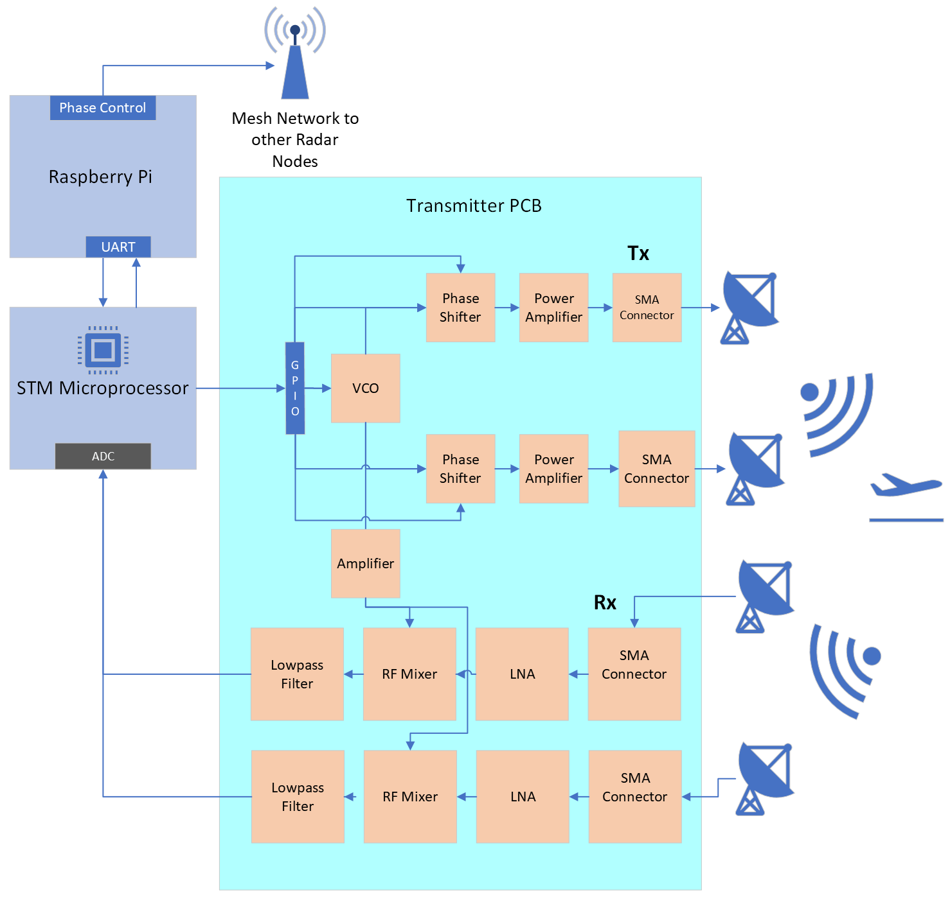
\includegraphics{Diagrams/overview.png}}
\caption{Architecture Overview}
\label{img:projoverview}
\end{figure}

In this chapter, we will go through the architecture of the PCB and show what parts we picked and what purposes they serve.
Figure \ref{img:projoverview} shows the overall architecture of the project.

\section{Voltage Controlled Oscillator (VCO)}
The first step in creating a radar is signal synthesis. You essentially need to create an alternating current signal that can
go through your antenna and radiate out into the air. To reiterate from Chapter \ref{Radar Theory}, higher frequency signals are
important for a better radar resolution, and so it is desired to have a signal that is high in frequency. Naively, at the
beginning of this project we thought we could use a 16 bit DAC to synthesize our signal but after finding out its max clock rate 
was 1 MHz, we realized a DAC was not fit for this. All we needed was something that could create a simple sinusoid at a very
high frequency.

Voltage Controlled Oscillators (VCO) do just this. They take in a "tuning voltage" which corresponds to a certain frequency
of sinusoid which it will output. The circuitry for this is beyond me, but for a good overall guide on VCOs you can check out
DigiKey's article \href{https://www.digikey.com/en/articles/the-basics-of-voltage-controlled-oscillators-vcos}{here}.

Now that we knew how to synthesize our signal, it was important to find a good VCO that had a high output bandwidth. Whatever
bandwidth the VCO has will impact what parts we can get in the other stages of the RF chain since these must be within the VCOs
operating regions. 

\begin{figure}[H]
    \centering
    \scalebox{.7}{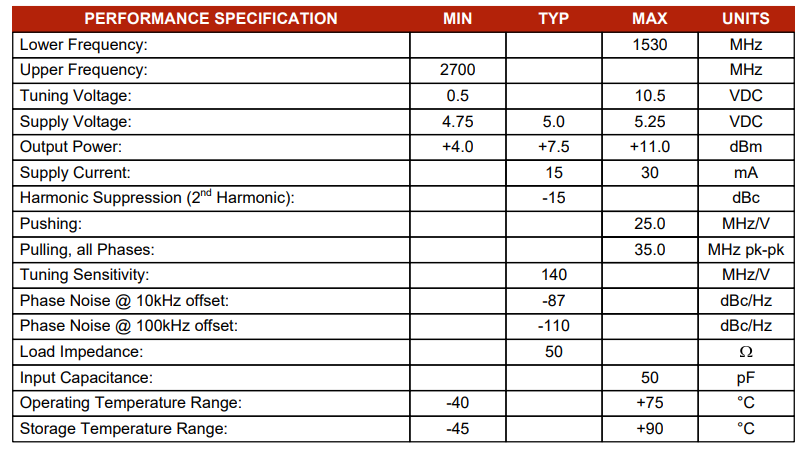
\includegraphics{DatasheetImages/vcotable.png}}
    \caption{VCO Datasheet Table}
    \label{img:vcotable}
\end{figure}
\begin{figure}[H]
    \centering
    \scalebox{.7}{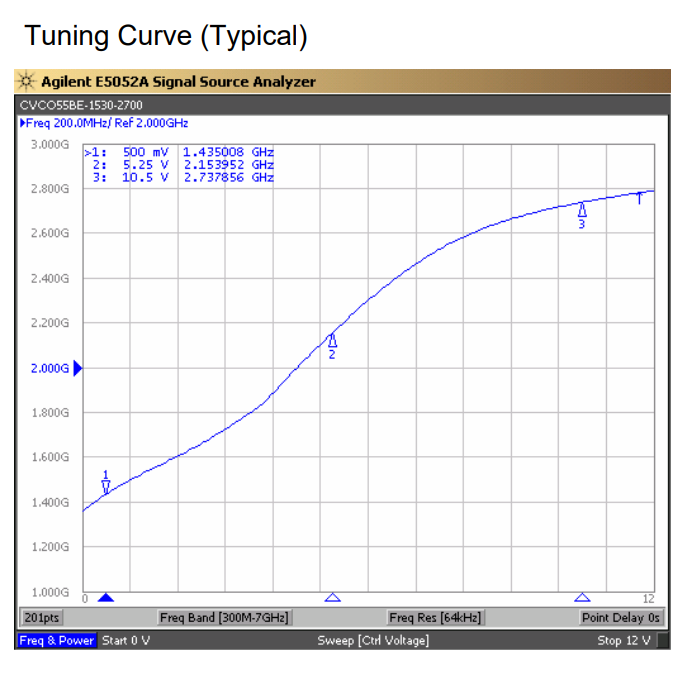
\includegraphics{DatasheetImages/vcotuningtable.png}}
    \caption{Tuning Voltage Graph}
    \label{img:tuninggraph}
\end{figure}

We chose a VCO from Crystek which can be found on Digikey \href{https://www.digikey.com/en/products/detail/crystek-corporation/CVCO55BE-1530-2700/1644030}{here}.
Looking at the specifications table in Figure \ref{img:vcotable}, some good things to look for are first and foremost the frequency
range of the part. It goes from about 1.5-2.7 GHz, which is a pretty wide range and would support a lot of other parts as it also
covers the Wi-Fi band. The second thing to look for is output power. The output power can be a constraint for other parts, since they
might have a absolute limit on their input power, and it is useful to know the output power for finding out how strong your signal will be
once it propogates out of your antenna. Here we can see the output power is around 7.5 dBm, and this will be split four ways. 
Decibels are a logarithmic scale, so we cannot just divide by four but instead use a decibel calculator like \href{https://noisetools.net/decibelcalculator}{this one}.

Now, another key metric is the tuning voltage. Luckily, this Crystek provides a tuning voltage graph found in Figure \ref{img:tuninggraph}
that shows us how the output frequency changes with changes in the tuning voltage. One observation is that it is not linear, meaning
our ramp voltage will not result in a true linear ramp in frequency. Another observation is that our chosen frequency of 1.8 GHz is
around 3.5 volts following the graph. Our STM board that will generate the ramp voltage can by default only go to 3.3 volts, but we
found a workaround to go to 5 volts which allowed us to stick with our decided center frequency.

\section{Power Divider}
As mentioned before, we want to divide the VCO's signal four ways because want it to go to two phase shifters, and two mixers.
At first we thought it was as simple as having one wire split into four, but as we will go over in Chapter \ref{PCB}, impedence
matching is very important in RF circuits. To put it simply, impedance matching ensures that no power is reflected, and this is
important because reflected power means distortions in the signal and power loss. That means we needed a power splitter meant for
splitting an RF signal without causing reflected power. There is not much of note with the part we used which can be found 
\href{https://www.mouser.com/ProductDetail/Mini-Circuits/WP4P1%2B?qs=Imq1NPwxi77kWybHhilv%2Fg%3D%3D}{here}. The main thing is that
it contains the frequency of 1.8 GHz we want to use.

\section{Phase Shifter}
Two of the power dividers split paths will go into phase shifters. The phase shifters are used to make our phased array
of antennas as explained in Chapter \ref{Radar Theory}. They are able to change the phase (add time delay), to the signal 
so that when they propogate through the air they can construct and destruct. The phase shifters we chose can be found
\href{https://www.digikey.com/en/products/detail/psemi/PE44820B-X/5822957}{here}. These are digital phase shifters that have 256
different phases it can apply to the signal. They have a parallel or serial interface we can use to transmit 8 bit words That
will alter the phase of our signal. The interface and its timing diagrams will be explained more in detail in Chapter \ref{Digital Processing}.
All we need to know is that the bandwidth that the chip supports contains 1.8 GHz.

\section{Power Amplifier}
\begin{figure}[H]
  \centering
  \scalebox{.6}{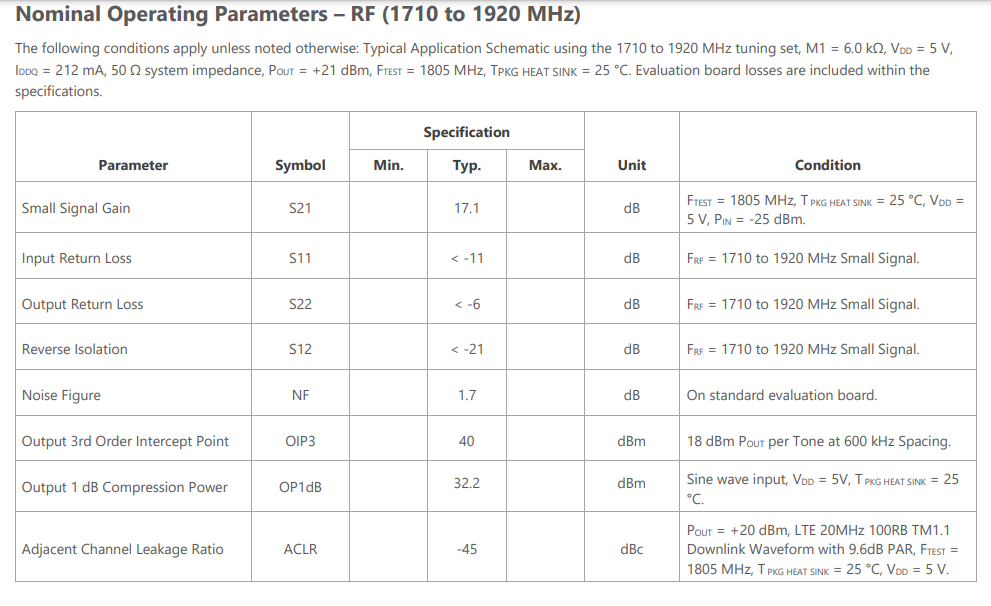
\includegraphics{DatasheetImages/poweramptable.png}}
  \caption{Power Amplifier Table}
  \label{img:poweramptable}
\end{figure}
At this point after the VCO and phase shifter, we want the RF signal to propogate through the air. However, according to the
radar range equation the power of the signal when attenuating through the air attenuates at a power of four which is a lot.
Therefore, we need to make sure our signal is powerful enough to go pretty far. So, we use an RF power amplifier to amplify the
signal. We chose a part from GuerillaRF which can be found \href{https://www.mouser.com/ProductDetail/Guerrilla-RF/GRF5112?qs=ulEaXIWI0c%252Bti188Qa1Now%3D%3D}{here}.
Looking at the table in Figure \ref{img:poweramptable}, we can see some key metrics when looking at power amplifiers. First,
of course we want to make sure it has a bandwidth that supports our chosen frequency of 1.8 GHz. Second, we want to look at the
small-signal gain and Output 1 dB Compression Point or OP1dB. The small-signal gain is the ideal gain that can be reached with a 
low power signal, and is listed as 17.1 dB. The OP1dB is a metric we did not know about and were thankful to find it. With most amplifiers,
gain operates linearly meaning whatever power your input signal is you just add the gain of the amplifier and this will be the resulting power of the signal.
However, at a certain point the amplifier saturates and does not operate linearly anymore, and will essentially cap-off its gain at
the OP1dB limit. For example, with the OP1dB being 32.2 dB, if I input a signal that was 30 dB I would expect a resulting signal of
47.1 dB but this would not be the case. The amplifier ceases to operate linearly after the 32.2 dB mark, and will both distort the signal
and output something weaker than expected. A lot of amplifiers will boast a high gain but have a low OP1dB, so this is definitely something to check for.

\section{Low Noise Amplifier}
\begin{figure}[H]
  \centering
  \scalebox{.7}{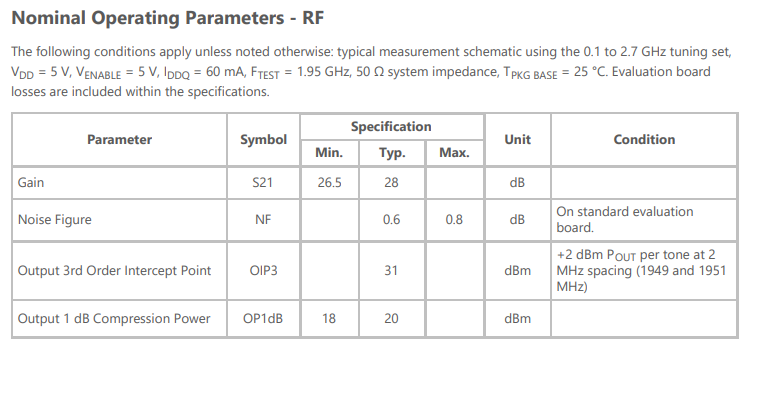
\includegraphics{DatasheetImages/lnatable.png}}
  \caption{Low-Noise Amplifier Table}
  \label{img:lnatable}
\end{figure}

This is the first part that will be placed in the receiver RF chain. According to the Friis equation in Chapter \ref{Radar Theory},
the first stage in the receiver RF chain matters a lot for the noise figure of your system. Therefore, we wanted to find a part
with a low noise figure and high gain, as this will impact our SNR the most. Low noise amplifiers are made for this exact purpose,
where they amplify a small signal with very low noise. The part we chose was \href{https://www.mouser.com/ProductDetail/Guerrilla-RF/GRF2133W?qs=ulEaXIWI0c%2FXgAPwqRmr2A%3D%3D}{this},
which is made by GuerillaRF. By examining the table in Figure \ref{img:lnatable}, we can see that it has a gain of 28 dB,
and a noise figure of .6 dB. We also can look at the OP1dB which has a figure of 20 dB. Since the LNA will be amplifying a signal
straight from an antenna, the signal will be super weak and there is a low likelihood it will reach the OP1dB.

\section{Mixer/LO Amp}
\begin{figure}[H]
  \centering
  \scalebox{.7}{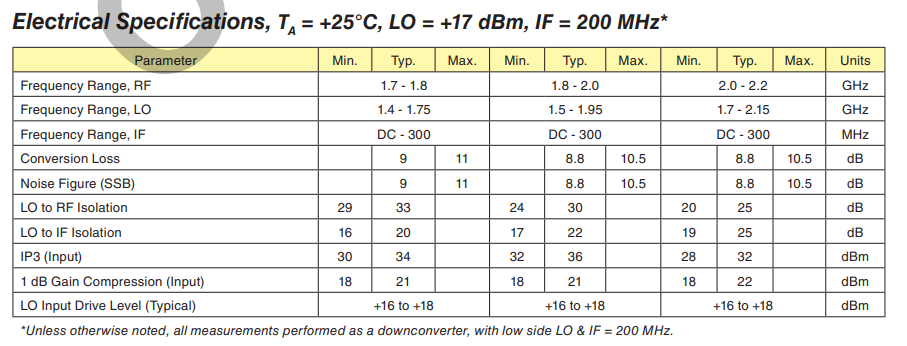
\includegraphics{DatasheetImages/mixertable.png}}
  \caption{Mixer Table}
  \label{img:mixertable}
\end{figure}
\begin{figure}[H]
  \centering
  \scalebox{.7}{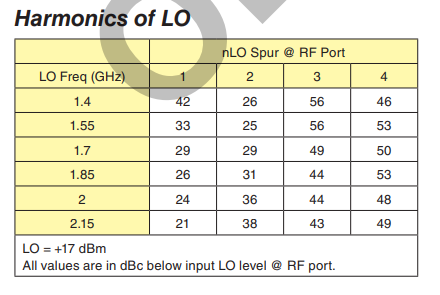
\includegraphics{DatasheetImages/mixerharmonics.png}}
  \caption{Mixer Harmonics Table}
  \label{img:mixerharmonics}
\end{figure}

Now that our received signal is amplified we must down-convert it in order to sample and process it. The process for doing
this is called heterodyning or mixing, and the theory behind this can be found in detail in Chapter \ref{Radar Theory}. 
A mixer has three ports, the local oscillator, RF signal, and output. The local oscillator and RF signal are multiplied
to produce the sum and difference of the LO and RF signals on the output port. We are mainly interested in the difference,
also called the Intermediate Frequency (IF) since it is a low frequency and can be sampled easily.
In our case, we take a copy of the VCO as the local oscillator and then mix this with the amplified return signal 
to produce our intermediate frequency. To achieve this, we used a discontinued mixer from Analog Devices which
can be found \href{https://www.arrow.com/en/products/hmc400ms8etr/analog-devices}{here}. 
Looking at the mixer's specifications table in Figure \ref{img:mixertable}, we can 
see some new properties. The conversion loss is the output IF power delivered minus the available RF input signal power. The
LO to RF Isolation is how much of the local oscillator signal leaks into the RF port, and the LO to IF Isolation is how much
the local oscillator signal leaks into the output port. This is a passive component, meaning it does not require power and
solely operates off the power of the LO and RF signals. Therefore we see in the table that the LO Input must be 16-18 dBm to drive
the mixer. Essentially the local oscillator powers the mixer, and its harmonics will therefore be prominent in the IF port due to
leakage. We can see in Figure \ref{img:mixerharmonics} that at 1.85 GHz the manufacturer tells us the strength of LO harmonics 
up to the fourth order. At the top it says spur which means spurious (unwanted) outputs due to the nonlinearity of the mixer.
Essentially this table tells us that there will be unwanted spectral components in the output, which is something we did not
pay enough attention to and will discuss in Chapter \ref{Issues}.
\begin{figure}[H]
  \centering
  \scalebox{.7}{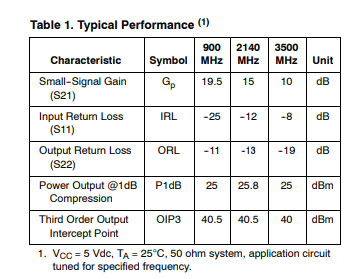
\includegraphics{DatasheetImages/loamptable.png}}
  \caption{LO Amp Table}
  \label{img:loamptable}
\end{figure}

As we said before, the mixer is a passive component which is driven by the LO which needs a power level of 16-18 dBm.
After splitting our VCO's output four ways, we have about a ~2 dBm signal that we must amplify. So, we chose an RF broadband
amplifier from NXP which can be found \href{https://www.digikey.com/en/products/detail/nxp-usa-inc/MMG3014NT1/1971761}{here}. As
we can see in Figure \ref{img:loamptable}, the amp has a gain of around 15 dB for our frequency and an OP1dB of 25.8 dB which is
a lot of headroom.

\section{IF Amplifiers and Filters}
Now, our return signal has been downconverted, but the power of that signal is very weak. As well as this, there are unwanted
spectral components in that signal that are bi-products of the mixer that we need to get rid of. This means we need amplifiers and
filters to make our signal ready to be sampled and processed in the microcontroller. First we used a super simple op-amp
that served as a voltage follower which can be found \href{https://www.digikey.com/en/products/detail/microchip-technology/MCP6001UT-I-OT/562450}{here}.
This was used to create a virtual ground for our biasing. Then we use a dual channel op-amp from TI for our variable gain
amplifier which can be found \href{https://www.mouser.com/ProductDetail/Texas-Instruments/LM2904DR?qs=5BZzbFV4k2vkQqOl3Q8qPg%3D%3D}{here}.

\begin{figure}[H]
  \centering
  \scalebox{.7}{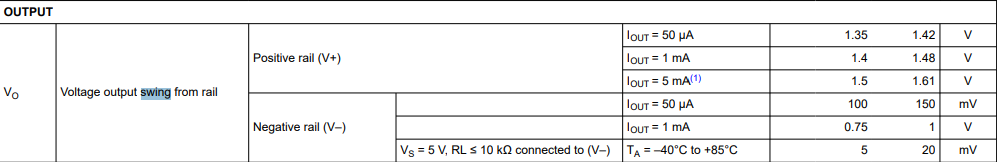
\includegraphics{DatasheetImages/outputswing.png}}
  \caption{Output Swing Characteristics}
  \label{img:outputswing}
\end{figure}

Honestly, when selecting parts we figured all operational amplifiers just acted the same way. However, after printing and manufacturing
we ran into problems which will be discussed in Chapter \ref{Issues} that could have been remedied if we paid more attention to
the Op-Amps we were using. The main problem is that these operational amplifiers are not "Rail-to-Rail".
While rail-to-rail amplifiers guarantee that they do not saturate until the positive and negative voltages you've supplied it,
other amplifiers have what is called voltage swing. As we can see in Figure \ref{img:outputswing}, the range of voltage
that the operational amplifier can achieve is not its rails, but specifies how much lower than its rail it will be. This is 
something to look out for when selecting an Op-Amp.

\begin{figure}[H]
  \centering
  \scalebox{.7}{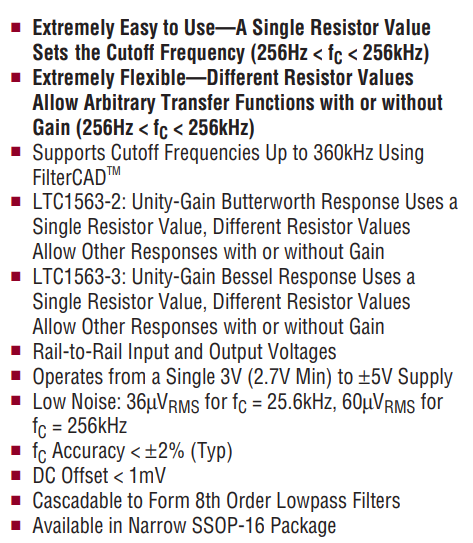
\includegraphics{DatasheetImages/filterspecs.png}}
  \caption{Filter Features}
  \label{img:filterspecs}
\end{figure}

After amplifying the signal, we wanted to filter out unwanted spectral components by using a strong filter. Instead of designing
this ourselves, we decided to use a 4th Order LPF which can be found \href{https://www.digikey.com/en/products/detail/analog-devices-inc/LTC1563-2IGN-PBF/962958}{here}.
By looking at Figure \ref{img:filterspecs}, we can see that this is an integrated circuit with a flexible cutoff frequency.
It also says that it is a rail-to-rail input and output circuit, which is an important feature to note as discussed with the amplifiers.
A fourth order filter just means that this filter has four filters with the same cutoff frequency cascaded upon each other, which
yields a steeper frequency response and attenuates are unwanted signals further.
\chapter{PCB
\index{Chapter!PCB}
\index{PCB}
\label{PCB}}
\chapter{Digital Processing
\index{Chapter!Digital Processing}
\index{Digital Processing}
\label{Digital Processing}}
\chapter{Networking
\index{Chapter!Networking}
\index{Networking}
\label{Networking}}


\chapter{Results
\index{Chapter!Results}
\index{Results}
\label{Results}}
\chapter{Issues
\index{Chapter!Issues}
\index{Issues}
\label{Issues}}

%\bibliography{bibfile}
%\bibliographystyle{unsrt}
%\bibliographystyle{IEEEtran}

%% Initial version by Darian Muresan, Ph.D.
% Edit and adjust as needed.

\documentclass[12pt]{cornell}

% add index support
\makeindex

% graphing programs
\usepackage{color}
\usepackage{psfrag}
\usepackage{verbatim}
\usepackage{fancyhdr}
\usepackage{minted}
%\usepackage{titlesec}
\usepackage{fancyvrb} 
% hyperlink programs
\usepackage[luatex, 
breaklinks=true, 
colorlinks=true,
citecolor=blue,
linkcolor=blue,
menucolor=black,
pagecolor=black,
urlcolor=blue
]{hyperref} % links in pdf
%\usepackage[colorlinks]{hyperref} % links in dvi
\usepackage{listings}
\usepackage{amsfonts} 
\usepackage{amssymb} 
%\usepackage{tabto}

\usepackage{tabularx,colortbl}
\usepackage[chapter]{algorithm} 
\usepackage{algorithmic} 
\usepackage{blindtext}
\usepackage{imakeidx}

% for electronics:
\usepackage[american]{circuitikz}

\definecolor{DarkGreen}{rgb}{0,0.6,0}
\definecolor{mygreen}{rgb}{0,0.6,0}
\definecolor{mygray}{rgb}{0.5,0.5,0.5}
\definecolor{mymauve}{rgb}{0.58,0,0.82}

\usepackage{tocloft}
\usepackage{amsmath}
\usepackage{tcolorbox}
\usepackage{enumitem}
\usepackage{longtable}
%\usepackage{textcomp}
\usepackage{txfonts}

%part for \part titles
%chap for \chapter titles
%sec for \section titles
%subsec for \subsection titles
%subsubsec for \subsubsection titles
%para for \paragraph titles
%subpara for \subparagraph titles
%fig for figure \caption titles
%subfig for subfigure \caption titles
%tab for table \caption titles
%subtab for subtable \caption titles

% update chapter number spacing
\setlength{\cftchapnumwidth}{2em}
\setlength{\cftsecnumwidth}{2.5em}
\setlength{\cftsubsecnumwidth}{3.5em}
\setlength{\cftsubsubsecnumwidth}{4.5em}

\addtolength{\cftsecindent}{0.5em}
\addtolength{\cftsubsecindent}{0.5em}
\addtolength{\cftsubsubsecindent}{0.5em}

%\titlespacing*{\chapter}{0pt}{-50pt}{20pt}
%\titleformat{\chapter}[display]{\normalfont\huge\bfseries}{\chaptertitlename\ 
%\thechapter}{20pt}{\Huge}
%\pagestyle{fancy}
%\pagestyle{cornell}
%
%\rhead{F054-021-0172}
%\chead{Nonlinear Enhancement of Visual Target Detection (AF05-T021)}
%\lhead{GSTI}
%\lfoot{\scriptsize Use or disclosure of data on this page is subject
%to the restriction on the title page of this proposal.}
%\cfoot{}
%\rfoot{\thepage}

\newfont{\Bp}{msbm10}
\newfont{\BpBig}{msbm10 scaled\magstep2}
\newfont{\Sc}{eusm10}
\newfont{\ScBig}{eusm10 scaled\magstep3}
\newfont{\Fr}{eufm10}
\newfont{\FrBig}{eufm10 scaled\magstep1}

% some commands:
\newcommand{\dxi}{{\tt m\_xDeltaInput}}
\newcommand{\dyi}{{\tt m\_yDeltaInput}}
\newcommand{\dci}{{\tt m\_cDeltaInput}}
\newcommand{\dxo}{{\tt m\_xDeltaOutput}}
\newcommand{\dyo}{{\tt m\_yDeltaOutput}}
\newcommand{\dco}{{\tt m\_cDeltaOutput}}
\newcommand{\ttf}[1]{{\tt #1}}
\newcommand{\tbl}[2]{{\begin{tabular}{c} #1 \\ #2 \end{tabular}}}

\newcommand{\urltwo}[2]{\mbox{\href{#1}{\tt #2}}}
\newcommand{\qnorm}[1]{\|#1\|_{\bQ}}
\newcommand{\qdot}[2]{\lrb #1, #2 \rrb_{\bQ}}
\newcommand{\kdot}[2]{\lrb #1, #2 \rrb_{\bf k}}
\newcommand{\tdot}[2]{\lrb #1, #2 \rrb}
\newcommand{\mydiff}[2]{\lrb #1 - #2 \rrb}
\newcommand{\lena}{\textit{lena}}
\newcommand{\barb}{\textit{barbara}}
\newcommand{\boat}{\textit{boat}}
\newcommand{\leaves}{\textit{leaves}}
\newcommand{\rings}{\textit{rings}}
\newcommand{\treg}{\textit{train region}}
\newcommand{\dreg}{\textit{denoise region}}
\newcommand{\oreg}{\textit{overlap region}}
\newcommand{\sil}{\sigma_l^2}
\newcommand{\sn}{\sigma^2}
\newcommand{\bn}{{\mbox{\bf \FrBig N}}}
\newcommand{\n}{\mbox{\Fr N}}
%\newcommand{\bn}{\bf N}
%\newcommand{\n}{N}
\newcommand{\bY}{\textbf{Y}}
\newcommand{\bX}{\textbf{X}}
\newcommand{\bb}{\textbf{b}}
\newcommand{\bu}{\textbf{u}}
\newcommand{\bv}{\textbf{v}}
\newcommand{\by}{\textbf{y}}
\newcommand{\bx}{\textbf{x}}
\newcommand{\be}{\textbf{e}}
\newcommand{\bz}{\textbf{z}}
\newcommand{\bs}{\textbf{s}}
\newcommand{\bw}{\textbf{w}}
\newcommand{\bQ}{\textbf{Q}}
\newcommand{\bphi}{\textbf{$\phi$}}
\newcommand{\lsb}{\left[}
\newcommand{\rsb}{\right]}
\newcommand{\lrb}{\left(}
\newcommand{\rrb}{\right)}
\newcommand{\lcb}{\left\{}
\newcommand{\rcb}{\right\}}
\newcommand{\R}{\mbox{\BpBig R}}
\newcommand{\F}{{\cal F}}
\newcommand{\Fk}{\mbox{\Sc F}}
\newcommand{\bQF}{\textbf{Q}_{\mbox{\Sc F}}}
\newcommand{\N}{{\cal N}}
\newcommand{\xlz}{X_l(z)}
\newcommand{\xhz}{X_h(z)}
\newcommand{\xz}{X(z)}
\newcommand{\pr}{ perfect reconstruction }
\newcommand{\smb}{Smith-Barnwell }
\newcommand{\xw}{X(e^{j\omega})}
\newcommand{\xmw}{X(-e^{j\omega})}
\newcommand{\dw}{D(e^{j\omega})}
\newcommand{\dmw}{D(-e^{j\omega})}
\newcommand{\ew}{E(e^{j\omega})}
\newcommand{\emw}{E(-e^{j\omega})}
\newcommand{\fw}{F_0(e^{j\omega})}
\newcommand{\fmw}{F_0(-e^{j\omega})}
\newcommand{\hoz}{H_1(z)}
\newcommand{\hzz}{H_0(z)}
\newcommand{\goz}{G_1(z)}
\newcommand{\gzz}{G_0(z)}
\newcommand{\hzw}{H_{0}(e^{j\omega})}
\newcommand{\hzmw}{H_{0}(-e^{j\omega})}
\newcommand{\hzcw}{H_{0}(e^{-j\omega})}
\newcommand{\how}{H_1(e^{j\omega})}
\newcommand{\homw}{H_1(-e^{j\omega})}
\newcommand{\gzw}{G_0(e^{j\omega})}
\newcommand{\gzmw}{G_0(-e^{j\omega})}
\newcommand{\gow}{G_1(e^{j\omega})}
\newcommand{\gomw}{G_1(-e^{j\omega})}
\newcommand{\wl}{e^{-jwL}}
\newcommand{\aqua}{\textit{AQua with OR }}
\newtheorem{theorem}{Theorem}
\newtheorem{lemma}{Lemma}
\newtheorem{corollary}{Corollary}
\newtheorem{claim}{Claim}
\newtheorem{definition}{Definition}
\newenvironment{proof}{\noindent{\em Proof.}}{\ \hfill Q.E.D.}
%\newtheorem{moduleCount}{L}
\newcommand*{\labelfile}[1]{%
  \label{file:#1}%
}

\lstset{ %
  backgroundcolor=\color{white},   % choose the background color; you must add \usepackage{color} or \usepackage{xcolor}
  basicstyle=\footnotesize,        % the size of the fonts that are used for the code
  breakatwhitespace=false,         % sets if automatic breaks should only happen at whitespace
  breaklines=true,                 % sets automatic line breaking
  captionpos=b,                    % sets the caption-position to bottom
  commentstyle=\color{DarkGreen},    % comment style
  deletekeywords={...},            % if you want to delete keywords from the given language
  escapeinside={\%*}{*)},          % if you want to add LaTeX within your code
  extendedchars=true,              % lets you use non-ASCII characters; for 8-bits encodings only, does not work with UTF-8
  %frame=single,                   % adds a frame around the code
  keepspaces=true,                 % keeps spaces in text, useful for keeping indentation of code (possibly needs columns=flexible)
  keywordstyle=\color{blue},       % keyword style
  language=C++,                    % the language of the code
  morekeywords={*,...},            % if you want to add more keywords to the set
  numbers=left,                    % where to put the line-numbers; possible values are (none, left, right)
  numbersep=5pt,                   % how far the line-numbers are from the code
  numberstyle=\tiny\color{mygray}, % the style that is used for the line-numbers
  rulecolor=\color{black},         % if not set, the frame-color may be changed on line-breaks within not-black text (e.g. comments (green here))
  showspaces=false,                % show spaces everywhere adding particular underscores; it overrides 'showstringspaces'
  showstringspaces=false,          % underline spaces within strings only
  showtabs=false,                  % show tabs within strings adding particular underscores
  stepnumber=1,                    % the step between two line-numbers. If it's 1, each line will be numbered
  stringstyle=\color{mymauve}     % string literal style
  %tabsize=2,                      % sets default tabsize to 2 spaces
  %caption=\lstname                % show the filename of files included with \lstinputlisting; also try caption instead of title
}

% Uncomment draftcopy to get the word DRAFT boldly across the first page
%   By the way, xdvi won't show it but it will come out when you print
%\usepackage[light,all]{draftcopy}		% DRAFT on first page
%\draftcopySetGrey{.97}
%\draftcopyName{Confidential}{150}
%\draftcopFirstPage{1}

% Uncomment drafthead to get the date and DRAFT in the header of pages
% that are normallly numbered on the top, pages 2-n of each chapter for example
% This doesn't work with centered page numbers: \pagestyle{cornellc}
%\usepackage{drafthead}

% Including selective chapters:
% use this to selectively process chapters, etc.  Put a % in front of
% the sections that you don't want done this time.  Includes are
% used instead of \input so that LaTeX will keep track of chapters and
% pages without processing everything.  Don't let any spaces creep in
% around the words or it will not work!


\includeonly{
prologue,
manIntroduction,
manProjectDescription,
manResources,
manRadarTheory,
manPartSelection,
manPCB,
manDigitalProcessing,
manNetworking,
manResults,
manIssues
}

\makeindex

\begin{document}

\pagenumbering{roman}
\singlespacing
% File: prologue.tex
% Thesis prologue:  Title page, acknowledgements, table of contents,
% list of figures, and list of tables.
%
% this file is to be \include'd after the \begin{document}

% Cornell-style title page
\begin{titlepage}
        \title{Mithril - FMCW Radar}
        \author{Tomas Esson, Ajay Thakkar, Juan Jimenez \\ tesson@stevens.edu, athakka5@stevens.edu, jjimene6@stevens.edu }
        \conferraldate{}{\today} \maketitle
\end{titlepage}

% Copyright page
%\begin{copyrightpage}
\makecopyright
%\end{copyrightpage}

% Abstract: the abstract body is pulled from the file abstract.tex;
%  the title is pulled from the \title command in the titlepage section

% Biographical information pulled from file bio.tex
%\begin{biosketch} \input bio \end{biosketch}

% Dedication (optional):  pulls information from file dedication.tex
%\begin{dedication} 
%\input dedicate 
%\end{dedication}

% Acknowledgements:  pulls information from file acknow
%\begin{acknowledgements} \input acknow \end{acknowledgements}

% Table of contents
\contentspage

% If you have no tables or figures put a % in front of the list page line
% List of tables
\tablelistpage

% List of figures
\figurelistpage



\setcounter{page}{1}        % set page counter
\pagenumbering{arabic}      % set page number style
\pagestyle{fancy}         % top right page numbers
%\pagestyle{cornell}
%\pagestyle{cornellc}       % centered page numbers, disables drafthead

\renewcommand{\chaptermark}[1]{\markboth{#1}{}}
\renewcommand{\sectionmark}[1]{\markright{#1}{}}

\fancyhead{} % clear all fields

\lhead{Chapter \thechapter}
%\lhead{\thechapter}
\chead{\leftmark}
\rhead{\thepage}


\lfoot{Chapter \thechapter}
\cfoot{\copyright Stevens -- \today \mbox{} -- FPGA Radio Receiver/Transmitter}
\rfoot{\thepage}

\renewcommand{\headrulewidth}{0.4pt}
\renewcommand{\footrulewidth}{0.4pt}

%\rhead{F054-021-0172}
%\chead{Nonlinear Enhancement of Visual Target Detection (AF05-T021)}
%\lhead{GSTI}
%\lfoot{\scriptsize Use or disclosure of data on this page is subject
%to the restriction on the title page of this proposal.}
%\cfoot{}
%\rfoot{\thepage}


\singlespacing
\chapter{Introduction 
\index{Chapter!Introduction}
\index{Introduction}
\label{Introduction}}

The following includes small biographies on all the authors as well as their research interests and projects.

\section*{Authors' Biographies}
\subsection*{Ajay Thakkar}
\textbf{Ajay Thakkar} Ajay Thakkar is a junior majoring in Computer Engineering. He is interested in signal processing and lower level coding. Below you can find his GitHub: \url{https://github.com/athakkar2}.

\subsection*{Tomas Esson}
\textbf{Tomas Esson} is an aspiring Computer Engineering at Stevens Institute of technology. He is an avid surfer and enjoys elegant math proofs. Currently pursuing interests in computer chip design, digital systems implementation, mathematical optimization of computer chips, and electrical engineering. 

\subsection*{Juan Jimenez}
\textbf{Juan Jimenez} is a Junior Computer Engineering student at the Stevens Institute of technology. Interested in the intersection between Artificial Intelligence, embedded electronics, and software engineering. To see more projects visit the following GitHub link: \url{https://github.com/jjimene1}  
\chapter{Project Description 
\index{Chapter!Project Description}
\index{Project Description}
\label{Project Description}}
\begin{figure}[H]
  \centering
  \begin{tikzpicture}[node distance = 2cm, auto]
      % Define block styles
      \tikzstyle{block} = [rectangle, draw, fill=blue!20, 
          text width=5em, text centered, rounded corners, minimum height=4em]
      \tikzstyle{line} = [draw, ->]
  
      % Place nodes
      \node [block] (mithril) {Mithril};
      \node [block, below of=mithril, node distance=4cm] (radar) {FMCW Radar};
      \node [block, left of=radar, node distance=4cm] (processing) {Digital Processing};
      \node [block, right of=radar, node distance=4cm] (networking) {Distributed Networking};
      \node [block, below of=processing, node distance=2cm] (STM) {STM MC and Python};
      \node [block, below of=radar, node distance=2cm] (ORCad) {Cadence ORCad};
      \node [block, below of=networking, node distance=2cm] (pi) {Raspberry Pi and MQTT};
      % Draw edges
      \path [line] (mithril) -- (radar);
      \path [line] (mithril) -- (processing);
      \path [line] (mithril) -- (networking);
      \path [line] (radar) -- (ORCad);
      \path [line] (processing) -- (STM);
      \path [line] (networking) -- (pi);
  \end{tikzpicture}
  \caption{Flowchart of the Mithril system}
  \label{fig:mithril_flowchart}
  \end{figure}
Mithril is a nodal FMCW radar system that incorporates traditional FMCW radar,
digital processing, edge computing, and distributed networking. The initial idea of this 

As can be seen in Figure \ref{fig:mithril_flowchart},
the radar was designed as a standalone PCB in ORCad, digital processing was handled by
STM microcontrollers, and distributed networking is done via Raspberry Pi's and the MQTT protocol.
All of these components were designed, engineered, and interfaced from scratch with a limited budget
of 2000 dollars.

\section{}
The heart of the project is a standalone PCB capable of FMCW radar.
\chapter{Resources
\index{Chapter!Resources}
\index{Resources}
\label{Resources}}
\chapter{Radar Theory
\index{Chapter!Radar Theory}
\index{Radar Theory}
\label{Radar Theory}}

\section{Getting Started}



include the benefits of using higher frequency signals

heterodyning
\chapter{Part Selection
\index{Chapter!Part Selection}
\index{Part Selection}
\label{Part Selection}}

\begin{figure}[H]
  \centering
  \scalebox{.8}{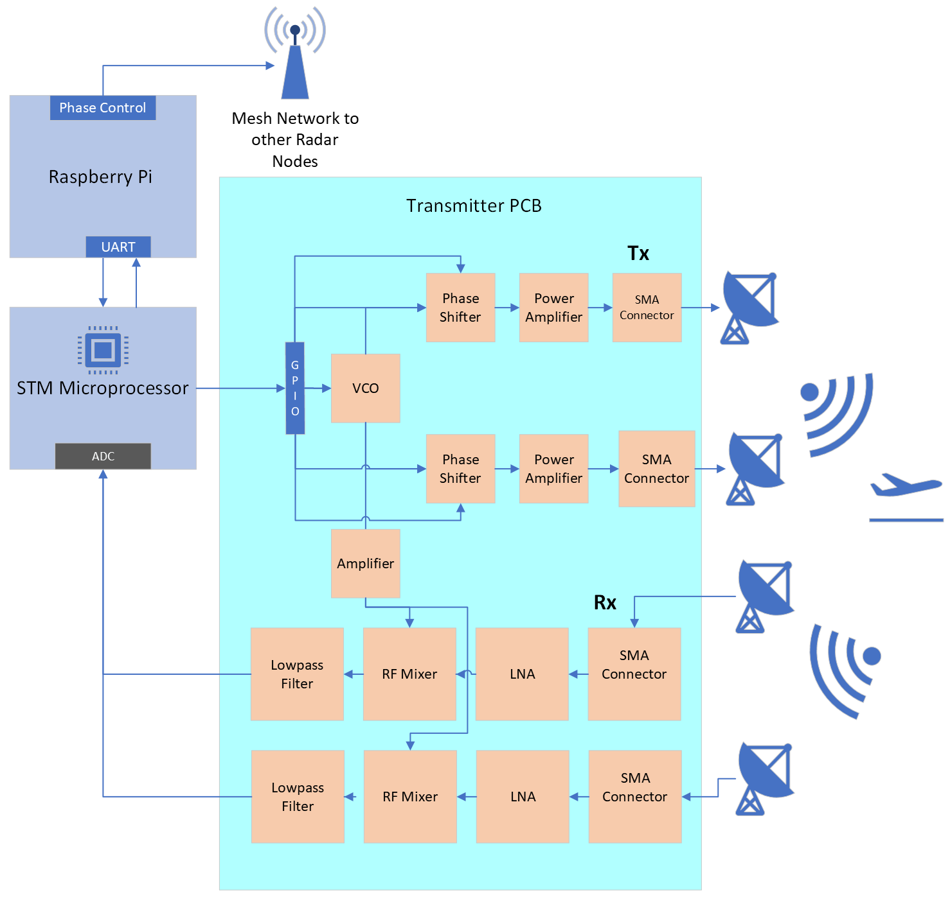
\includegraphics{Diagrams/overview.png}}
\caption{Architecture Overview}
\label{img:projoverview}
\end{figure}

In this chapter, we will go through the architecture of the PCB and show what parts we picked and what purposes they serve.
Figure \ref{img:projoverview} shows the overall architecture of the project.

\section{Voltage Controlled Oscillator (VCO)}
The first step in creating a radar is signal synthesis. You essentially need to create an alternating current signal that can
go through your antenna and radiate out into the air. To reiterate from Chapter \ref{Radar Theory}, higher frequency signals are
important for a better radar resolution, and so it is desired to have a signal that is high in frequency. Naively, at the
beginning of this project we thought we could use a 16 bit DAC to synthesize our signal but after finding out its max clock rate 
was 1 MHz, we realized a DAC was not fit for this. All we needed was something that could create a simple sinusoid at a very
high frequency.

Voltage Controlled Oscillators (VCO) do just this. They take in a "tuning voltage" which corresponds to a certain frequency
of sinusoid which it will output. The circuitry for this is beyond me, but for a good overall guide on VCOs you can check out
DigiKey's article \href{https://www.digikey.com/en/articles/the-basics-of-voltage-controlled-oscillators-vcos}{here}.

Now that we knew how to synthesize our signal, it was important to find a good VCO that had a high output bandwidth. Whatever
bandwidth the VCO has will impact what parts we can get in the other stages of the RF chain since these must be within the VCOs
operating regions. 

\begin{figure}[H]
    \centering
    \scalebox{.7}{\includegraphics{DatasheetImages/vcotable.png}}
    \caption{VCO Datasheet Table}
    \label{img:vcotable}
\end{figure}
\begin{figure}[H]
    \centering
    \scalebox{.7}{\includegraphics{DatasheetImages/vcotuningtable.png}}
    \caption{Tuning Voltage Graph}
    \label{img:tuninggraph}
\end{figure}

We chose a VCO from Crystek which can be found on Digikey \href{https://www.digikey.com/en/products/detail/crystek-corporation/CVCO55BE-1530-2700/1644030}{here}.
Looking at the specifications table in Figure \ref{img:vcotable}, some good things to look for are first and foremost the frequency
range of the part. It goes from about 1.5-2.7 GHz, which is a pretty wide range and would support a lot of other parts as it also
covers the Wi-Fi band. The second thing to look for is output power. The output power can be a constraint for other parts, since they
might have a absolute limit on their input power, and it is useful to know the output power for finding out how strong your signal will be
once it propogates out of your antenna. Here we can see the output power is around 7.5 dBm, and this will be split four ways. 
Decibels are a logarithmic scale, so we cannot just divide by four but instead use a decibel calculator like \href{https://noisetools.net/decibelcalculator}{this one}.

Now, another key metric is the tuning voltage. Luckily, this Crystek provides a tuning voltage graph found in Figure \ref{img:tuninggraph}
that shows us how the output frequency changes with changes in the tuning voltage. One observation is that it is not linear, meaning
our ramp voltage will not result in a true linear ramp in frequency. Another observation is that our chosen frequency of 1.8 GHz is
around 3.5 volts following the graph. Our STM board that will generate the ramp voltage can by default only go to 3.3 volts, but we
found a workaround to go to 5 volts which allowed us to stick with our decided center frequency.

\section{Power Divider}
As mentioned before, we want to divide the VCO's signal four ways because want it to go to two phase shifters, and two mixers.
At first we thought it was as simple as having one wire split into four, but as we will go over in Chapter \ref{PCB}, impedence
matching is very important in RF circuits. To put it simply, impedance matching ensures that no power is reflected, and this is
important because reflected power means distortions in the signal and power loss. That means we needed a power splitter meant for
splitting an RF signal without causing reflected power. There is not much of note with the part we used which can be found 
\href{https://www.mouser.com/ProductDetail/Mini-Circuits/WP4P1%2B?qs=Imq1NPwxi77kWybHhilv%2Fg%3D%3D}{here}. The main thing is that
it contains the frequency of 1.8 GHz we want to use.

\section{Phase Shifter}
Two of the power dividers split paths will go into phase shifters. The phase shifters are used to make our phased array
of antennas as explained in Chapter \ref{Radar Theory}. They are able to change the phase (add time delay), to the signal 
so that when they propogate through the air they can construct and destruct. The phase shifters we chose can be found
\href{https://www.digikey.com/en/products/detail/psemi/PE44820B-X/5822957}{here}. These are digital phase shifters that have 256
different phases it can apply to the signal. They have a parallel or serial interface we can use to transmit 8 bit words That
will alter the phase of our signal. The interface and its timing diagrams will be explained more in detail in Chapter \ref{Digital Processing}.
All we need to know is that the bandwidth that the chip supports contains 1.8 GHz.

\section{Power Amplifier}
\begin{figure}[H]
  \centering
  \scalebox{.6}{\includegraphics{DatasheetImages/poweramptable.png}}
  \caption{Power Amplifier Table}
  \label{img:poweramptable}
\end{figure}
At this point after the VCO and phase shifter, we want the RF signal to propogate through the air. However, according to the
radar range equation the power of the signal when attenuating through the air attenuates at a power of four which is a lot.
Therefore, we need to make sure our signal is powerful enough to go pretty far. So, we use an RF power amplifier to amplify the
signal. We chose a part from GuerillaRF which can be found \href{https://www.mouser.com/ProductDetail/Guerrilla-RF/GRF5112?qs=ulEaXIWI0c%252Bti188Qa1Now%3D%3D}{here}.
Looking at the table in Figure \ref{img:poweramptable}, we can see some key metrics when looking at power amplifiers. First,
of course we want to make sure it has a bandwidth that supports our chosen frequency of 1.8 GHz. Second, we want to look at the
small-signal gain and Output 1 dB Compression Point or OP1dB. The small-signal gain is the ideal gain that can be reached with a 
low power signal, and is listed as 17.1 dB. The OP1dB is a metric we did not know about and were thankful to find it. With most amplifiers,
gain operates linearly meaning whatever power your input signal is you just add the gain of the amplifier and this will be the resulting power of the signal.
However, at a certain point the amplifier saturates and does not operate linearly anymore, and will essentially cap-off its gain at
the OP1dB limit. For example, with the OP1dB being 32.2 dB, if I input a signal that was 30 dB I would expect a resulting signal of
47.1 dB but this would not be the case. The amplifier ceases to operate linearly after the 32.2 dB mark, and will both distort the signal
and output something weaker than expected. A lot of amplifiers will boast a high gain but have a low OP1dB, so this is definitely something to check for.

\section{Low Noise Amplifier}
\begin{figure}[H]
  \centering
  \scalebox{.7}{\includegraphics{DatasheetImages/lnatable.png}}
  \caption{Low-Noise Amplifier Table}
  \label{img:lnatable}
\end{figure}

This is the first part that will be placed in the receiver RF chain. According to the Friis equation in Chapter \ref{Radar Theory},
the first stage in the receiver RF chain matters a lot for the noise figure of your system. Therefore, we wanted to find a part
with a low noise figure and high gain, as this will impact our SNR the most. Low noise amplifiers are made for this exact purpose,
where they amplify a small signal with very low noise. The part we chose was \href{https://www.mouser.com/ProductDetail/Guerrilla-RF/GRF2133W?qs=ulEaXIWI0c%2FXgAPwqRmr2A%3D%3D}{this},
which is made by GuerillaRF. By examining the table in Figure \ref{img:lnatable}, we can see that it has a gain of 28 dB,
and a noise figure of .6 dB. We also can look at the OP1dB which has a figure of 20 dB. Since the LNA will be amplifying a signal
straight from an antenna, the signal will be super weak and there is a low likelihood it will reach the OP1dB.

\section{Mixer/LO Amp}
\begin{figure}[H]
  \centering
  \scalebox{.7}{\includegraphics{DatasheetImages/mixertable.png}}
  \caption{Mixer Table}
  \label{img:mixertable}
\end{figure}
\begin{figure}[H]
  \centering
  \scalebox{.7}{\includegraphics{DatasheetImages/mixerharmonics.png}}
  \caption{Mixer Harmonics Table}
  \label{img:mixerharmonics}
\end{figure}

Now that our received signal is amplified we must down-convert it in order to sample and process it. The process for doing
this is called heterodyning or mixing, and the theory behind this can be found in detail in Chapter \ref{Radar Theory}. 
A mixer has three ports, the local oscillator, RF signal, and output. The local oscillator and RF signal are multiplied
to produce the sum and difference of the LO and RF signals on the output port. We are mainly interested in the difference,
also called the Intermediate Frequency (IF) since it is a low frequency and can be sampled easily.
In our case, we take a copy of the VCO as the local oscillator and then mix this with the amplified return signal 
to produce our intermediate frequency. To achieve this, we used a discontinued mixer from Analog Devices which
can be found \href{https://www.arrow.com/en/products/hmc400ms8etr/analog-devices}{here}. 
Looking at the mixer's specifications table in Figure \ref{img:mixertable}, we can 
see some new properties. The conversion loss is the output IF power delivered minus the available RF input signal power. The
LO to RF Isolation is how much of the local oscillator signal leaks into the RF port, and the LO to IF Isolation is how much
the local oscillator signal leaks into the output port. This is a passive component, meaning it does not require power and
solely operates off the power of the LO and RF signals. Therefore we see in the table that the LO Input must be 16-18 dBm to drive
the mixer. Essentially the local oscillator powers the mixer, and its harmonics will therefore be prominent in the IF port due to
leakage. We can see in Figure \ref{img:mixerharmonics} that at 1.85 GHz the manufacturer tells us the strength of LO harmonics 
up to the fourth order. At the top it says spur which means spurious (unwanted) outputs due to the nonlinearity of the mixer.
Essentially this table tells us that there will be unwanted spectral components in the output, which is something we did not
pay enough attention to and will discuss in Chapter \ref{Issues}.
\begin{figure}[H]
  \centering
  \scalebox{.7}{\includegraphics{DatasheetImages/loamptable.png}}
  \caption{LO Amp Table}
  \label{img:loamptable}
\end{figure}

As we said before, the mixer is a passive component which is driven by the LO which needs a power level of 16-18 dBm.
After splitting our VCO's output four ways, we have about a ~2 dBm signal that we must amplify. So, we chose an RF broadband
amplifier from NXP which can be found \href{https://www.digikey.com/en/products/detail/nxp-usa-inc/MMG3014NT1/1971761}{here}. As
we can see in Figure \ref{img:loamptable}, the amp has a gain of around 15 dB for our frequency and an OP1dB of 25.8 dB which is
a lot of headroom.

\section{IF Amplifiers and Filters}
Now, our return signal has been downconverted, but the power of that signal is very weak. As well as this, there are unwanted
spectral components in that signal that are bi-products of the mixer that we need to get rid of. This means we need amplifiers and
filters to make our signal ready to be sampled and processed in the microcontroller. First we used a super simple op-amp
that served as a voltage follower which can be found \href{https://www.digikey.com/en/products/detail/microchip-technology/MCP6001UT-I-OT/562450}{here}.
This was used to create a virtual ground for our biasing. Then we use a dual channel op-amp from TI for our variable gain
amplifier which can be found \href{https://www.mouser.com/ProductDetail/Texas-Instruments/LM2904DR?qs=5BZzbFV4k2vkQqOl3Q8qPg%3D%3D}{here}.

\begin{figure}[H]
  \centering
  \scalebox{.7}{\includegraphics{DatasheetImages/outputswing.png}}
  \caption{Output Swing Characteristics}
  \label{img:outputswing}
\end{figure}

Honestly, when selecting parts we figured all operational amplifiers just acted the same way. However, after printing and manufacturing
we ran into problems which will be discussed in Chapter \ref{Issues} that could have been remedied if we paid more attention to
the Op-Amps we were using. The main problem is that these operational amplifiers are not "Rail-to-Rail".
While rail-to-rail amplifiers guarantee that they do not saturate until the positive and negative voltages you've supplied it,
other amplifiers have what is called voltage swing. As we can see in Figure \ref{img:outputswing}, the range of voltage
that the operational amplifier can achieve is not its rails, but specifies how much lower than its rail it will be. This is 
something to look out for when selecting an Op-Amp.

\begin{figure}[H]
  \centering
  \scalebox{.7}{\includegraphics{DatasheetImages/filterspecs.png}}
  \caption{Filter Features}
  \label{img:filterspecs}
\end{figure}

After amplifying the signal, we wanted to filter out unwanted spectral components by using a strong filter. Instead of designing
this ourselves, we decided to use a 4th Order LPF which can be found \href{https://www.digikey.com/en/products/detail/analog-devices-inc/LTC1563-2IGN-PBF/962958}{here}.
By looking at Figure \ref{img:filterspecs}, we can see that this is an integrated circuit with a flexible cutoff frequency.
It also says that it is a rail-to-rail input and output circuit, which is an important feature to note as discussed with the amplifiers.
A fourth order filter just means that this filter has four filters with the same cutoff frequency cascaded upon each other, which
yields a steeper frequency response and attenuates are unwanted signals further.
\chapter{PCB
\index{Chapter!PCB}
\index{PCB}
\label{PCB}}
\chapter{Digital Processing
\index{Chapter!Digital Processing}
\index{Digital Processing}
\label{Digital Processing}}
\chapter{Networking
\index{Chapter!Networking}
\index{Networking}
\label{Networking}}


\chapter{Results
\index{Chapter!Results}
\index{Results}
\label{Results}}
\chapter{Issues
\index{Chapter!Issues}
\index{Issues}
\label{Issues}}

%\bibliography{bibfile}
%\bibliographystyle{unsrt}
%\bibliographystyle{IEEEtran}

%% Initial version by Darian Muresan, Ph.D.
% Edit and adjust as needed.

\documentclass[12pt]{cornell}

% add index support
\makeindex

% graphing programs
\usepackage{color}
\usepackage{psfrag}
\usepackage{verbatim}
\usepackage{fancyhdr}
\usepackage{minted}
%\usepackage{titlesec}
\usepackage{fancyvrb} 
% hyperlink programs
\usepackage[luatex, 
breaklinks=true, 
colorlinks=true,
citecolor=blue,
linkcolor=blue,
menucolor=black,
pagecolor=black,
urlcolor=blue
]{hyperref} % links in pdf
%\usepackage[colorlinks]{hyperref} % links in dvi
\usepackage{listings}
\usepackage{amsfonts} 
\usepackage{amssymb} 
%\usepackage{tabto}

\usepackage{tabularx,colortbl}
\usepackage[chapter]{algorithm} 
\usepackage{algorithmic} 
\usepackage{blindtext}
\usepackage{imakeidx}

% for electronics:
\usepackage[american]{circuitikz}

\definecolor{DarkGreen}{rgb}{0,0.6,0}
\definecolor{mygreen}{rgb}{0,0.6,0}
\definecolor{mygray}{rgb}{0.5,0.5,0.5}
\definecolor{mymauve}{rgb}{0.58,0,0.82}

\usepackage{tocloft}
\usepackage{amsmath}
\usepackage{tcolorbox}
\usepackage{enumitem}
\usepackage{longtable}
%\usepackage{textcomp}
\usepackage{txfonts}

%part for \part titles
%chap for \chapter titles
%sec for \section titles
%subsec for \subsection titles
%subsubsec for \subsubsection titles
%para for \paragraph titles
%subpara for \subparagraph titles
%fig for figure \caption titles
%subfig for subfigure \caption titles
%tab for table \caption titles
%subtab for subtable \caption titles

% update chapter number spacing
\setlength{\cftchapnumwidth}{2em}
\setlength{\cftsecnumwidth}{2.5em}
\setlength{\cftsubsecnumwidth}{3.5em}
\setlength{\cftsubsubsecnumwidth}{4.5em}

\addtolength{\cftsecindent}{0.5em}
\addtolength{\cftsubsecindent}{0.5em}
\addtolength{\cftsubsubsecindent}{0.5em}

%\titlespacing*{\chapter}{0pt}{-50pt}{20pt}
%\titleformat{\chapter}[display]{\normalfont\huge\bfseries}{\chaptertitlename\ 
%\thechapter}{20pt}{\Huge}
%\pagestyle{fancy}
%\pagestyle{cornell}
%
%\rhead{F054-021-0172}
%\chead{Nonlinear Enhancement of Visual Target Detection (AF05-T021)}
%\lhead{GSTI}
%\lfoot{\scriptsize Use or disclosure of data on this page is subject
%to the restriction on the title page of this proposal.}
%\cfoot{}
%\rfoot{\thepage}

\newfont{\Bp}{msbm10}
\newfont{\BpBig}{msbm10 scaled\magstep2}
\newfont{\Sc}{eusm10}
\newfont{\ScBig}{eusm10 scaled\magstep3}
\newfont{\Fr}{eufm10}
\newfont{\FrBig}{eufm10 scaled\magstep1}

% some commands:
\newcommand{\dxi}{{\tt m\_xDeltaInput}}
\newcommand{\dyi}{{\tt m\_yDeltaInput}}
\newcommand{\dci}{{\tt m\_cDeltaInput}}
\newcommand{\dxo}{{\tt m\_xDeltaOutput}}
\newcommand{\dyo}{{\tt m\_yDeltaOutput}}
\newcommand{\dco}{{\tt m\_cDeltaOutput}}
\newcommand{\ttf}[1]{{\tt #1}}
\newcommand{\tbl}[2]{{\begin{tabular}{c} #1 \\ #2 \end{tabular}}}

\newcommand{\urltwo}[2]{\mbox{\href{#1}{\tt #2}}}
\newcommand{\qnorm}[1]{\|#1\|_{\bQ}}
\newcommand{\qdot}[2]{\lrb #1, #2 \rrb_{\bQ}}
\newcommand{\kdot}[2]{\lrb #1, #2 \rrb_{\bf k}}
\newcommand{\tdot}[2]{\lrb #1, #2 \rrb}
\newcommand{\mydiff}[2]{\lrb #1 - #2 \rrb}
\newcommand{\lena}{\textit{lena}}
\newcommand{\barb}{\textit{barbara}}
\newcommand{\boat}{\textit{boat}}
\newcommand{\leaves}{\textit{leaves}}
\newcommand{\rings}{\textit{rings}}
\newcommand{\treg}{\textit{train region}}
\newcommand{\dreg}{\textit{denoise region}}
\newcommand{\oreg}{\textit{overlap region}}
\newcommand{\sil}{\sigma_l^2}
\newcommand{\sn}{\sigma^2}
\newcommand{\bn}{{\mbox{\bf \FrBig N}}}
\newcommand{\n}{\mbox{\Fr N}}
%\newcommand{\bn}{\bf N}
%\newcommand{\n}{N}
\newcommand{\bY}{\textbf{Y}}
\newcommand{\bX}{\textbf{X}}
\newcommand{\bb}{\textbf{b}}
\newcommand{\bu}{\textbf{u}}
\newcommand{\bv}{\textbf{v}}
\newcommand{\by}{\textbf{y}}
\newcommand{\bx}{\textbf{x}}
\newcommand{\be}{\textbf{e}}
\newcommand{\bz}{\textbf{z}}
\newcommand{\bs}{\textbf{s}}
\newcommand{\bw}{\textbf{w}}
\newcommand{\bQ}{\textbf{Q}}
\newcommand{\bphi}{\textbf{$\phi$}}
\newcommand{\lsb}{\left[}
\newcommand{\rsb}{\right]}
\newcommand{\lrb}{\left(}
\newcommand{\rrb}{\right)}
\newcommand{\lcb}{\left\{}
\newcommand{\rcb}{\right\}}
\newcommand{\R}{\mbox{\BpBig R}}
\newcommand{\F}{{\cal F}}
\newcommand{\Fk}{\mbox{\Sc F}}
\newcommand{\bQF}{\textbf{Q}_{\mbox{\Sc F}}}
\newcommand{\N}{{\cal N}}
\newcommand{\xlz}{X_l(z)}
\newcommand{\xhz}{X_h(z)}
\newcommand{\xz}{X(z)}
\newcommand{\pr}{ perfect reconstruction }
\newcommand{\smb}{Smith-Barnwell }
\newcommand{\xw}{X(e^{j\omega})}
\newcommand{\xmw}{X(-e^{j\omega})}
\newcommand{\dw}{D(e^{j\omega})}
\newcommand{\dmw}{D(-e^{j\omega})}
\newcommand{\ew}{E(e^{j\omega})}
\newcommand{\emw}{E(-e^{j\omega})}
\newcommand{\fw}{F_0(e^{j\omega})}
\newcommand{\fmw}{F_0(-e^{j\omega})}
\newcommand{\hoz}{H_1(z)}
\newcommand{\hzz}{H_0(z)}
\newcommand{\goz}{G_1(z)}
\newcommand{\gzz}{G_0(z)}
\newcommand{\hzw}{H_{0}(e^{j\omega})}
\newcommand{\hzmw}{H_{0}(-e^{j\omega})}
\newcommand{\hzcw}{H_{0}(e^{-j\omega})}
\newcommand{\how}{H_1(e^{j\omega})}
\newcommand{\homw}{H_1(-e^{j\omega})}
\newcommand{\gzw}{G_0(e^{j\omega})}
\newcommand{\gzmw}{G_0(-e^{j\omega})}
\newcommand{\gow}{G_1(e^{j\omega})}
\newcommand{\gomw}{G_1(-e^{j\omega})}
\newcommand{\wl}{e^{-jwL}}
\newcommand{\aqua}{\textit{AQua with OR }}
\newtheorem{theorem}{Theorem}
\newtheorem{lemma}{Lemma}
\newtheorem{corollary}{Corollary}
\newtheorem{claim}{Claim}
\newtheorem{definition}{Definition}
\newenvironment{proof}{\noindent{\em Proof.}}{\ \hfill Q.E.D.}
%\newtheorem{moduleCount}{L}
\newcommand*{\labelfile}[1]{%
  \label{file:#1}%
}

\lstset{ %
  backgroundcolor=\color{white},   % choose the background color; you must add \usepackage{color} or \usepackage{xcolor}
  basicstyle=\footnotesize,        % the size of the fonts that are used for the code
  breakatwhitespace=false,         % sets if automatic breaks should only happen at whitespace
  breaklines=true,                 % sets automatic line breaking
  captionpos=b,                    % sets the caption-position to bottom
  commentstyle=\color{DarkGreen},    % comment style
  deletekeywords={...},            % if you want to delete keywords from the given language
  escapeinside={\%*}{*)},          % if you want to add LaTeX within your code
  extendedchars=true,              % lets you use non-ASCII characters; for 8-bits encodings only, does not work with UTF-8
  %frame=single,                   % adds a frame around the code
  keepspaces=true,                 % keeps spaces in text, useful for keeping indentation of code (possibly needs columns=flexible)
  keywordstyle=\color{blue},       % keyword style
  language=C++,                    % the language of the code
  morekeywords={*,...},            % if you want to add more keywords to the set
  numbers=left,                    % where to put the line-numbers; possible values are (none, left, right)
  numbersep=5pt,                   % how far the line-numbers are from the code
  numberstyle=\tiny\color{mygray}, % the style that is used for the line-numbers
  rulecolor=\color{black},         % if not set, the frame-color may be changed on line-breaks within not-black text (e.g. comments (green here))
  showspaces=false,                % show spaces everywhere adding particular underscores; it overrides 'showstringspaces'
  showstringspaces=false,          % underline spaces within strings only
  showtabs=false,                  % show tabs within strings adding particular underscores
  stepnumber=1,                    % the step between two line-numbers. If it's 1, each line will be numbered
  stringstyle=\color{mymauve}     % string literal style
  %tabsize=2,                      % sets default tabsize to 2 spaces
  %caption=\lstname                % show the filename of files included with \lstinputlisting; also try caption instead of title
}

% Uncomment draftcopy to get the word DRAFT boldly across the first page
%   By the way, xdvi won't show it but it will come out when you print
%\usepackage[light,all]{draftcopy}		% DRAFT on first page
%\draftcopySetGrey{.97}
%\draftcopyName{Confidential}{150}
%\draftcopFirstPage{1}

% Uncomment drafthead to get the date and DRAFT in the header of pages
% that are normallly numbered on the top, pages 2-n of each chapter for example
% This doesn't work with centered page numbers: \pagestyle{cornellc}
%\usepackage{drafthead}

% Including selective chapters:
% use this to selectively process chapters, etc.  Put a % in front of
% the sections that you don't want done this time.  Includes are
% used instead of \input so that LaTeX will keep track of chapters and
% pages without processing everything.  Don't let any spaces creep in
% around the words or it will not work!


\includeonly{
prologue,
manIntroduction,
manProjectDescription,
manResources,
manRadarTheory,
manPartSelection,
manPCB,
manDigitalProcessing,
manNetworking,
manResults,
manIssues
}

\makeindex

\begin{document}

\pagenumbering{roman}
\singlespacing
\include{prologue}

\setcounter{page}{1}        % set page counter
\pagenumbering{arabic}      % set page number style
\pagestyle{fancy}         % top right page numbers
%\pagestyle{cornell}
%\pagestyle{cornellc}       % centered page numbers, disables drafthead

\renewcommand{\chaptermark}[1]{\markboth{#1}{}}
\renewcommand{\sectionmark}[1]{\markright{#1}{}}

\fancyhead{} % clear all fields

\lhead{Chapter \thechapter}
%\lhead{\thechapter}
\chead{\leftmark}
\rhead{\thepage}


\lfoot{Chapter \thechapter}
\cfoot{\copyright Stevens -- \today \mbox{} -- FPGA Radio Receiver/Transmitter}
\rfoot{\thepage}

\renewcommand{\headrulewidth}{0.4pt}
\renewcommand{\footrulewidth}{0.4pt}

%\rhead{F054-021-0172}
%\chead{Nonlinear Enhancement of Visual Target Detection (AF05-T021)}
%\lhead{GSTI}
%\lfoot{\scriptsize Use or disclosure of data on this page is subject
%to the restriction on the title page of this proposal.}
%\cfoot{}
%\rfoot{\thepage}


\singlespacing
\include{manIntroduction}
\include{manProjectDescription}
\include{manResources}
\include{manRadarTheory}
\include{manPartSelection}
\include{manPCB}
\include{manDigitalProcessing}
\include{manNetworking}
\include{manResults}
\include{manIssues}

%\bibliography{bibfile}
%\bibliographystyle{unsrt}
%\bibliographystyle{IEEEtran}

%\input{manual.ind}
\printindex
\end{document}

\printindex
\end{document}

\printindex
\end{document}

\printindex
\end{document}
